% !TeX spellcheck = en_US
\documentclass[11pt, fleqn, titlepage]{article}
%\usepackage{siunitx}
\usepackage{SpeedyGonzales}
\usepackage{MediocreMike}
\newcommand{\so}[2]{{#1}\mathrm{e}{#2}}
% \geometry{top=1cm}
%\usepackage{cleveref}
\usepackage{tablefootnote}
\usepackage{hyperref}
\usepackage{array}
\usepackage{amsmath}
%\usepackage[bottom]{footmisc}
\usepackage{ragged2e}
\usepackage{booktabs}
\usepackage{lipsum}
\usepackage{csquotes}
\usepackage{longtable}
\usepackage{arydshln}
\usepackage{subcaption}
\usepackage{listings}
\usepackage{nccmath}
\usepackage{pxfonts}
\usepackage{array}
\usepackage{multirow}
\usepackage{enumitem}
\usepackage{color}
\usepackage{booktabs}
\usepackage{makecell}
\usepackage{multicol}
\usepackage{nccmath}
\usepackage{graphicx}
\usepackage[utf8]{inputenc}
\usepackage{xcolor}
\usepackage{dsfont}
\usepackage[htt]{hyphenat}
\lstset{basicstyle=\ttfamily,
	showstringspaces=false,
	commentstyle=\color{red},
	keywordstyle=\color{blue},
	breaklines=true,
	postbreak=\mbox{\textcolor{red}{$\hookrightarrow$}\space}
}

\hypersetup{
	colorlinks=true,
	linkcolor=blue,
	filecolor=magenta,      
	urlcolor=cyan,
}

\newcommand{\norm}[1]{\left\lVert#1\right\rVert}
\newcommand\graybox[1]{\colorbox{lightgray}{\ttfamily #1}}

% Variables for result plots
\newcommand\skipper{1.4pt}
\newcommand\ripper{2.5pt}

% Variables for result plots
\newcommand\skipperer{0.45pt}
\newcommand\ripperer{1.25pt}

\newcommand\bigskipx{2.1pt}
\newcommand\bigskipy{3.75pt}

\newcommand{\1}[1]{\mathds{1}\left[#1\right]}

%%%%%%% Setup for python code in latex %%%%%%%
% Default fixed font does not support bold face
\DeclareFixedFont{\ttb}{T1}{txtt}{bx}{n}{12} % for bold
\DeclareFixedFont{\ttm}{T1}{txtt}{m}{n}{12}  % for normal

% Custom colors
\usepackage{color}
\definecolor{deepblue}{rgb}{0,0,0.5}
\definecolor{deepred}{rgb}{0.6,0,0}
\definecolor{deepgreen}{rgb}{0,0.5,0}

\usepackage{listings}

% Python style for highlighting
\newcommand\pythonstyle{\lstset{
		language=Python,
		tabsize=2,
		basicstyle=\ttm,
		morekeywords={self},              % Add keywords here
		keywordstyle=\ttb\color{deepblue},
		emph={MyClass,__init__},          % Custom highlighting
		emphstyle=\ttb\color{deepred},    % Custom highlighting style
		stringstyle=\color{deepgreen},
		frame=tb,                         % Any extra options here
		showstringspaces=false,
		literate={\ \ }{{\ }}1
}}

% Python for external files
\newcommand\pythonexternal[2][]{{
\pythonstyle
\lstinputlisting[#1]{#2}}}

%%%% Define table citing %%%%
\usepackage{letltxmacro,etoolbox}

\LetLtxMacro{\originalcite}{\cite}
\def\tablecite#1#{%
	\def\pretablecite{#1}%
	\tableciteaux}
\def\tableciteaux#1{%
	\textsuperscript{\expandafter\originalcite\pretablecite{#1}}%
}
\AtBeginEnvironment{table}{\let\cite\tablecite}


\title{CycleGAN for Removing Field Strength Bias in Alzheimer's Disease Classification Model}
\author{Oskar Eiler Wiese Christensen \& Anders Henriksen \\ \texttt{\{s183917, s183904\}@dtu.dk}}
\date{\today}

\pagestyle{plain}
\fancyhf{}
\rfoot{Page \thepage{} of \pageref{LastPage}}

\graphicspath{{imgs/}}

\begin{document}
\maketitle
\begin{abstract}
	\small
	\noindent
	The progression of Alzheimer's Disease is slow and lead to death within 7-10 years from the date of diagnosis. In addition, AD is the most common precursor to dementia in Denmark, and an estimated 85000-90000 people live with a dementia disease. \noindent As such, methods for diagnosis have been researched for many decades, especially within the field of medical imaging. 
	\noindent
	A previous study exploring the possibility of classifying AD from MRI images stemming from the ADNI database showed promising results in classifying the disease, however, a bias between the magnetic field strength of the images used in the study was demonstrated. To eliminate the demonstrated bias, this project implements a CycleGAN to translate between 1.5T \& 3T MRI scans in order to generate 1.5T version of 3T images and vice versa to retrain a classifier to classify AD without the observed magnetic field strength bias. The project finds that a CycleGAN model can successfully be trained to translate between the magnetic field strength domains quantified by a RMSE difference of 0.85064 when mapping from 3T to 1.5T and 0.9243 when mapping from 1.5T to 3T, compared to the baseline. Furthermore, when inspecting the feature representation of a classifier trained purely on original 1.5T \& 3T images in a two-dimensional space, by utilizing t-SNE and forward passing cycleGAN generated images along with original images, no significant difference in their distributions can be determined. Based on RMSE, t-SNE and visual inspection, the generated images demonstrate utmost close resemblance to real images. 
	% Konklussion på at data fra cycleGAN kan bruges til at træne en biasfri classifier
	Moreover, the synthetically generated data seems promising in training an unbiased classifier to predict AD. Contingent on the t-SNE plots, the classifier exhibits no bias towards the magnetic field strength.
	% This implies that --> cycleGAN help cure AD
	Based on the amount of resources society spends on AD \& dementia, a successful prediction model will economically drive down cost and improve life quality and expectancy of future AD patients. 
	\noindent
	The findings of the project implies that a combination of a cycleGAN \& deep learning classifier might help reduce the severity of AD for a multitude of generations to come and in the long run may aid in finding a cure or reason as to how \& why AD occurs. 
	
	

	%TODO hav baseline accuracy inde i resultater fig loss for classifers 
	
\end{abstract}


%	\small
%	\noindent
%	Unfair treatment is deeply ingrained in many cultures and awareness of this is only just now starting to rise up. After the display of rage against the system and oppression seen in America during the spring and summer of 2020, it is obvious that discrimination has no place in a first world country. To that same extent, machine learning models that have been trained on biased datasets based on people's actions also need to have the discrimination corrected to avoid generally unfair treatment. One significant case is that of the COMPAS dataset and algorithm by Northpointe Inc. for determining chance to re-offend for defendants on trial. This algorithm was scrutinized by ProPublica for having a bias of applying higher risk scores to African-Americans than to Caucasians. To find and eliminate the bias in the COMPAS dataset for this project, a feed forward neural network was implemented to predict the recidivism score. Bias in the dataset was proven by separating the protected groups of the data and analyzing whether their false positive and true positive rates are equal and plotting the ROC-curves of each group of different classification thresholds of the model. The project finds that the model has inherited three biases, one of which is discussed and found by ProPublicas analysis, which is the racial bias against African-Americans. Furthermore, a sexist and age bias towards men and young individuals is also proven in this project. Equal opportunity and equalized odds from Hardt et al.'s paper was used to correct for any such bias found in the model \cite{equal_of_oppor}. Correcting for this bias lead to a tiny change in accuracy, which shows that not correcting for bias is nonsensical. Bias correction should be enforced and used in the entire field of AI to ensure fairness and general application of ML models. More studies on the subject need to surface, and enforcement needs to be applied in the field to make sure that bias has in fact been removed or attempted to be removed. If the future of AI and ML keeps going like it has so far, bias will never be truly removed, and the ugly roots of racism and sexism found in many cultures will resurface. As seen all over the world as of the summer of 2020, discrimination will not be tolerated and unenforced models with poor or no bias correction will result in response from society, peaceful or otherwise. 


\vspace*{-4cm}

\section*{Glossary}

\begin{table}[H]\label{fig:files}
	\hspace*{-2cm}
	\begin{tabular}{l l l l l l l l l}
		\toprule
		& \textbf{Term} & & & & & & \textbf{Explanation}                                              & \\ \midrule
		& AD            & & & & & & Alzheimer's Disease                                               & \\
		& ADNI          & & & & & & Alzheimer's Disease Neuroimaging Initiative                       & \\
		& AI            & & & & & & Artificial Intelligence                                           & \\
		& Adam          & & & & & & Adaptive Moment Estimation                                        & \\
		& BCE           & & & & & & Binary Cross-Entropy                                              & \\
		& CN            & & & & & & cognitively normal                                                & \\
		& CNN           & & & & & & Convolutional Neural Network                                      & \\
		& CRS           & & & & & & Coordinate Reference System                                       & \\
		& CSF           & & & & & & Cerebrospinal Fluid                                               & \\
		& CycleGAN      & & & & & & Cyclic Generative Adversarial Network                             & \\
		& DKK           & & & & & & Danish Kroner                                                     & \\
		& DL            & & & & & & Deep Learning                                                     & \\
		& DTU           & & & & & & Technical University of Denmark                                   & \\
		& EM-GCA        & & & & & & Electromagnetic Gaussian Classifier Array                         & \\
		& FS            & & & & & & FreeSurfer                                                        & \\
		& GAN           & & & & & & Generative Adversarial Network                                    & \\
		& GCA           & & & & & & Gaussian Classifier Array                                         & \\
		& GPU           & & & & & & Graphics Processing Unit                                          & \\
		& HPC           & & & & & & High Performance Computing                                        & \\
		& KL            & & & & & & Kullback-Liebler                                                  & \\
		& LONI          & & & & & & Laboratory of Neuro Imaging                                       & \\
		& MCI           & & & & & & Mild Cognitive Impairment                                         & \\
		& ML            & & & & & & Machine learning                                                  & \\
		& MNI           & & & & & & Montreal Neurological Institute                                   & \\
		& MNIST         & & & & & & Modified National Institute of Standards and Technology database  & \\
		& MRI           & & & & & & Magnetic Resonance Imaging                                        & \\
		& NA            & & & & & & Not Applicable                                                    & \\
		& PCA           & & & & & & Principal Component Analysis                                      & \\
		& PET           & & & & & & Positron Emission Tomography                                      & \\
		& RGB           & & & & & & Red-Green-Blue                                                    & \\
		& RMSE          & & & & & & Root-Mean-Square Error                                            & \\
		& ReLU          & & & & & & Rectified Linear Unit                                             & \\
		& SVD           & & & & & & Singular Value Decomposition                                      & \\
		& WGAN          & & & & & & Wasserstein GAN                                                   & \\
		& fMRI          & & & & & & Functional Magnetic Resonance Imaging                             & \\
		& kSVM-DT       & & & & & & kernel support vector machine decision trees                      & \\
		& t-SNE         & & & & & & t-Distributed Stochastic Neighbor Embedding                       & \\
		
		
		
		\bottomrule
	\end{tabular}
\end{table}

{
\hypersetup{linkcolor=black}
\newpage
\tableofcontents 
\newpage
}

\section{Introduction} \label{indledning}
% Indeholde purpose / formål med projekt
%TODO skal skrives om 
Alzheimer’s Disease (AD) is a disease which, in the year 2021, affected an
estimated 5.8 million people aged 65 years or older in America alone. By the
time an individual shows early symptoms of AD, whether by a screening test
or a physical measurement of the brain volume, it is already too late to prevent the rapid development of the disease. Thus, to decrease cost of treatment
and increase chance of successful rehabilitation, it is becoming ever increasingly
important to detect AD. Many studies has been conducted within the field of Alzheimer's with magnetic resonance imaging (MRI) scans stored
in the Alzheimers’s Disease Neuroimaging Initiative (ADNI). The MRI scans
range from an electromagnetic field of 1.5 tesla (T) to 3T. The quality of the 3T
images is higher, but the price unfortunately follows this same trend, meaning that MRI electromagnetic field strength is determined mostly by funding. This could, inherently, introduce a bias in an algorithm trained on a dataset with MRI images
spanning both magnetic field strengths, resulting in images with different levels
of detail. Previous studies have attempted to create a binary classifier for Alzheimer's with the tools of machine learning and computer vision, however, a bias between the magnetic field strength of images was found by Kergel \cite{CamillaKandidat}, which was illustrated by projecting high dimensional features of the model into a two dimensional space using t-distributed stochastic neighbor embedding, see figure \ref{fig:camillatsne}.

\begin{figure}[H]
	\centering
	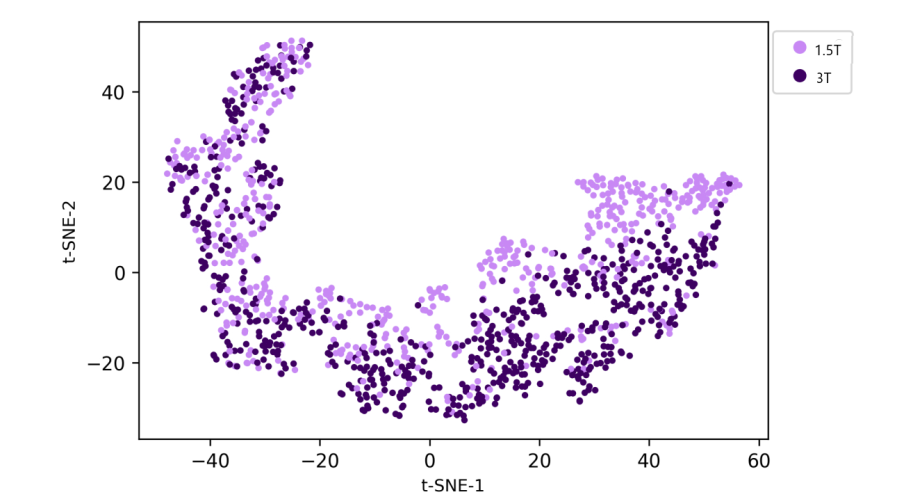
\includegraphics[width=0.6\linewidth]{imgs/camilla_tsne}
	\caption{T-distributed stochastic neighbor embedding from Camilla Kergel Pedersen: Demographic bias in public neuroimaging databases, and its
		effect on AI systems for computer-aided diagnosis \cite{CamillaKandidat}.}
	\label{fig:camillatsne}
\end{figure}

\subsection{Incentive of the Project}
%TODO: SKal der mere vægt på at gøre 3T til 1.5T-billeder?
The scope of this project will be to train a classifier on MRI images to predict AD as well as training a cycle-generative adversarial network (CycleGAN)
to generate 1.5T images from 3T images in order to construct more usable, and
hopefully unbiased, data. Thereby, the model will have more available training
data, which should lead to a more generalizable classifier, which will be able to aid doctors and humans in need all around the world. This project will also aim to determine possible bias introduced in the model and discuss how a classifier can be implemented as a tool for doctors. Furthermore, the project will discuss how this might benefit AD prevention, reduce treatment cost and the possible ethical scenarios that might be at play.
\\\\
The project will revolve around the possibility to predict Alzheimer's by utilizing CycleGAN generated data. Furthermore, the questions below will be researched in detail.

\begin{itemize}
	\item[\textbf{i}] Can a CycleGAN be trained to map between the following domains: 1.5T and 3T MRI
	images?
	
	\item[\textbf{ii}] How effective is the training progress in a prediction model when predicting whether a patient has
	Alzheimer’s disease? And can the CycleGAN data remove previous demonstrated bias from the model?
	
	\item[\textbf{iii}] Will the CycleGAN have any societal and economic impacts
	given the success of the prediction model?
	
\end{itemize}

\subsection{State of the Art}\label{statens_kunst}
% Statens kunst
In recent years, many attempts have been made to both classify and detect Alzheimer's Disease (AD). Many different approaches to this classification problem has been taken. However, as computers get better and the field of machine learning and deep learning grows, an arsenal of new methods to predict and classify AD at early stages have been proposed as of late. This section aims to highlight some of finest work within this field of study, demonstrating the current stage and methods used to approach the classification problem. 
\\\\
\noindent
A novel approach was proposed by Zhang et al. in 2014, using kernel support vector machine decision trees (kSVM-DT). In this study, they use basic preprocessing as well as principle component analysis for feature extraction. On the basis of these extracted features, the kSVM-DT was constructed. The proposed model has an 80\% classification accuracy. Furthermore, the computation of classifying a subject is relatively fast, taking 0.022 seconds \cite{yudong}. 
\\\\
Another approach was taken by Suk and Shen using a stacked auto-encoder. Their method was different from previous methods which focused mainly on low-level features such as gray matter tissue volumes from MRI. A stacked auto-encoder can represent complicated features such as non-linear relationships. Combining the low-level features with latent information, they created a robust model for classification achiving 95.9\% accuracy and 75.8\% prediction accuracy of MCI to AD conversion \cite{suk_and_shen_1}. In 2015, the work was extended and they achieved an accuracy of  98.8\% for AD/CN classification and 83.7\% accuracy for prediction of MCI to AD conversion. This was done with greedy layer-wise pre-training and fine-tuning of the deep learning model \cite{suk_and_shen_2}.
\\\\
Recently, convolutional neural networks (CNN) have been showing promising results for AD prediction. In general CNNs have been a widely implemented method within the field of image recognition. Cheng et al. proposes to construct multi-level CNNs to gradually learn and combine the multi-modality features for AD classification using MRI and PET images. An accuracy of 89.6\% was achieved using this method. \cite{cheng}

Basaia et al. achieved the highest measured accuracy on the ADNI1 data with a CNN classifier. The highest rate achieved was 99\%. Thus, concluding that CNNs serves as a powerful method for Alzheimer's diagnostics. Furthermore, the model demonstrated good predictions with no prior feature engineering nor variability of imaging protocols, and Basaia et al. concludes that it is likely to be a generalizable model even on unseen patient data \cite{neuro}. 

\subsection{Contributions}

This report aim to give an approachable account of the possibility of using CycleGANs to translate between the 1.5T and 3T domains. Furthermore, it aims to remove the inherent bias of using the two types of images in deep learning models. As such, the reader can expect to get the following from the study:

\begin{itemize}
	\item Illustrations which show an overview of the data in the different parts of the preprocessing pipeline. What does it look like? How is it done?
	
	\item A GAN will be provided in a Jupyter Notebook for easy access. Furthermore, an equivalent model has been run and the results and discussion are added to the appendix of this paper. This aims to give the reader important insight into the mathematical intuition behind the GAN.
	
	\item Five different CycleGANs will be presented, both through text and mathematical definition, and implemented in order to show the effect of the model as a bias corrections tool and to see how efficacious the CycleGAN actually is in mapping between the domains.
	
	\item To put the other contributions into a real-world context, an ethical and societal discussion of the CycleGAN and a classifier will be carried out. 
	
	\item Code for the preprocessing, the implementation of the CycleGANs as well as a section on reproducibility will be provided in the interest of making the results of this paper both as replicable and as reliable as possible. The section on reproducibility supplies the reader with the used seeds, packages, versions of packages and a thorough explanation of the code used in the project.
\end{itemize}
\noindent
The general goal of the contributions given above is to create a model which can remove previously demonstrated biases. Furthermore, the report also aims to give an overview of the implication of a successful CycleGAN within the Alzheimer's and medical research area. The economic incentives, societal impact and ethical considerations will all be touched upon in the discussion of this paper. 

\section{Background}

This section will contain relevant information in regards to understanding and reproducing the project presented. It will shortly introduce magnetic resonance imaging, magnetic field strength, some trade offs of using MRI scanners and MNI space. 
%TODO: referér til hver subsection

\subsection{Magnetic Resonance Imaging (MRI)}
%TODO simple explanation of MRI scans
MRI is a technique developed through the 1970s and 1980s. The scanner itself can be seen on figure \ref{fig:mriscanner}. In simple terms, an MRI scanner works by inducing a magnetic field to a patient. The magnetic field will then excite the atoms within an area of the subject's brain. The resulting signal is then measured by the scanner \cite{mri}.  
\begin{figure}[H]
	\centering
	\includegraphics[width=0.7\linewidth]{imgs/mri_scanner}
	\caption{A classic MRI scanner from MART PRODUCTION. Original image can be found \href{https://www.pexels.com/photo/technology-hospital-medicine-indoors-7089017/}{here}. }
	\label{fig:mriscanner}
\end{figure}
\noindent
MRI was originally called nuclear magnetic resonance imaging, but was later readopted as MRI due to \textit{"nuclear"} having negative associations with the field of research \cite{wiki} \cite{mri2}.

\subsection{Magnetic Field Strength}
%TODO simple explanation of THE TESLAz
It is inherently import to understand the underlying concept and difference of the magnetic field strength of the MRI scanner in use. In this project, two types of images are used: 1.5T and 3T images. Tesla is a unit in which the strength of a magnetic field can be measured. The stronger the magnetic resonance, the more detailed the MRI image. The strength of the magnetic field can be thought of as reducing the amount of noise in the image and adding more clarity. Thus this is like increasing the resolution of a normal RGB image. The 3T images are also constructed with more expensive machines and are not available in all countries nor hospitals around the world. This amplifies the need for a method to translate between these domains. 

\subsection{Trade off of Using MRI}
%TODO Talk about voxels ( a voxel and encode information about two distinct areas in the brain in same number.see: https://www.youtube.com/watch?v=6wxJ1up-E7E&list=PLIQIswOrUH6_DWy5mJlSfj6AWY0y9iUce )

MRI data is constructed from an MR scanner in the form of volumes. These 3D images can be compared to centicubes, which together form a big square, where the brain is inside. Each centicube in this image is often referred to as a voxel, and each voxel contains a value that represents the intensity value in the specific area - see figure \ref{fig:voxel}. For T1 weighted or structural images, this determines the boundary between gray matter \& white matter from cerebrospinal fluid. In T2 weighted images, it represents more active voxels to  less active voxels. However, voxels do have certain issues e.g. a voxel can encompass information about two anatomically distinct areas, like if a voxel encompasses two different gyri. Furthermore, it is hard to measure structural properties such as gray matter thickness or volume, which might be important for AD classification. FreeSurfer Software can help by turning the 3D representation into a 2D representation using triangles. The points of the triangles are vertices and they are connected by an edge. Each vertex then contain measurements such as gray matter volume and thickness, area, curvature etc. These surfaces can be inflated to visualize where MRI activations and gray matter differences are located more precisely than the voxel representation would have allowed for. 

\begin{figure}[H]
	\centering
	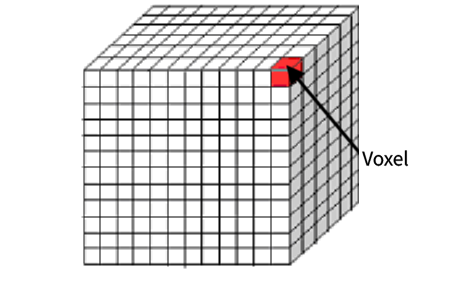
\includegraphics[width=0.42\linewidth]{imgs/voxel}
	\caption{A cube that represents the grid in which the subject brain is located. Each voxel will contain information about the intensity of the area. This representation is prone to loss since one voxel can contain information about multiple areas of the brain.}
	\label{fig:voxel}
\end{figure}



\subsection{MNI Space}
%TODO explain the MNI space 
Montreal Neurological Institute 305 (MNI305) is an atlas for brain mapping which was introduced by Evans et al. in 1992. The mapping was created from 250 normal subjects that have been MRI scanned. It is a known method for normalization and is an often-used industry practice for an average human brain \cite{evans}. 

The atlas was constructed in two steps. Firstly, anatomical landmarks were outlined for each subject manually. The landmarks were found using the Talairach atlas, which is a 3 dimensional coordinate system used to map several areas of the brain, independently of the brain volume and shape. Secondly, each MRI volume from the patients were mapped to an average MRI from the previous subjects, to reduce impact of order effect. %TODO: Hvad er order effect?
The mapping was performed with whole-brain linear (9-parameter) image similarity residual and not according to Talairach's piece-wise linear model \cite{collins}. 

Thus, they created a space, namely the MNI305 space, which is used in this project. The space is useful to compare the brain of different subjects and for a deep learning model to learn meaningful feature representations of such images. 


\section{Data} 
%TODO Look at histogram distribution, types of images, etc etc etc etc
%TODO Look at age distribution of subjects in data and also put which subjects
%TODO: Lav en introduktion og referér til undersektionerne


The data used in this project is from the Alzheimer's Disease Neurosurgical Initiative (ADNI). This initiative unites researchers with study data to investigate and define the progression of Alzheimer's Disease (AD). 
ADNI collects, validates and utilizes data, including (MRI), positron emission tomography (PET), genetics, cognitive tests, cerebrospinal fluid (CSF) biomarkers and blood biomarkers as predictors of the disease \cite{adni}.
More specifically, this project will use MRI data from ADNI 1 \& 2, which was launched in October 24, 2004. Originally, this project was designed to find more accurate biomarkers for the early detection of AD.
The ADNI project analyzed more than a thousand different brain scans from three different subject groups, namely, subjects with mild cognitive impairment (MCI), subjects with early AD and and cognitively normal (CN) subjects \cite{adni1}. 
\\\\
All of the data used from the ADNI database can be downloaded here: \url{https://ida.loni.usc.edu/} \newline
This website is owned by Laboratory of Neuro Imaging (LONI). The core philosophy of LONI is \blockcquote{loni}{to increase the pace of discovery in neuroscience by better understanding of how the brain works when it is healthy and what goes wrong in disease}.


\subsection{Data Demographics}
%subj_id, age, etc. etc. - dette skal findes et sted på server eller ADNI hjemmeside 
To get an understanding of some of the summary statistics of subjects in this project, the figure and table below have been constructed. From figure \ref{fig:age}, it can be seen that the average subject age is 73.3 years. Furthermore, the proportion of men to women is close to 50\%. The potential for an inherent gender bias is thus low considering the ratio of men to women is almost equal.

\begin{table}[H]
	\begin{tabular}{llllll}
		& CN&\ \ AD\ \ MCI &\ \ Other &\ \ Total   \\
		N & 698&\ \ 377\ \ 634 &\ \ 473 &\ \ 2182   \\
		Male/Female & 300/398&\ \ 196/181\ \ 389/245 &\ \ 243/229  &\ \ 1128/1053   \\
		Age & 75.1&\ \ 73.24\ \ 74.1 &\ \ 71.2 &\ \ 73.3   \\
	\end{tabular}
\end{table}


\begin{figure}[H]
	\centering
	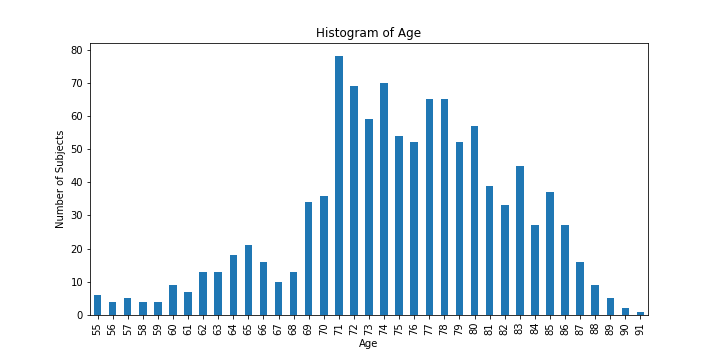
\includegraphics[width=0.9\linewidth]{imgs/age_distro}
	\caption{A histogram of the age distribution among the subjects in ADNI1 and ADNI2 \cite{adni,adni1}.}
	\label{fig:age}
\end{figure}


\subsection{Description of Data} \label{dataDescription}

%Description of how images(raw) obtained from patients, number of images, type of subjects  

The images from the ADNI dataset are from several different subjects and a plethora of studies around the world.
Each of the patients have had multiple scans throughout the span of the ADNI project, however in this project, only use the baseline scan, the first subject MRI scan, will be utilized. 
The MRI scans are three dimensional images of the subjects brain. 
The original image is in a \texttt{.mgz} file format which is a compressed \texttt{mgh} file. 
This file format can store 3D-images along with headers containing information about the subject and a transformation matrix.
The raw images stem from the original analysis from 2004 and onwards. There are in total 1562 %TODO perhaps more perhaps less? 
unique brain scans, all of which are used in this project.

\begin{figure}[H]
	\centering
	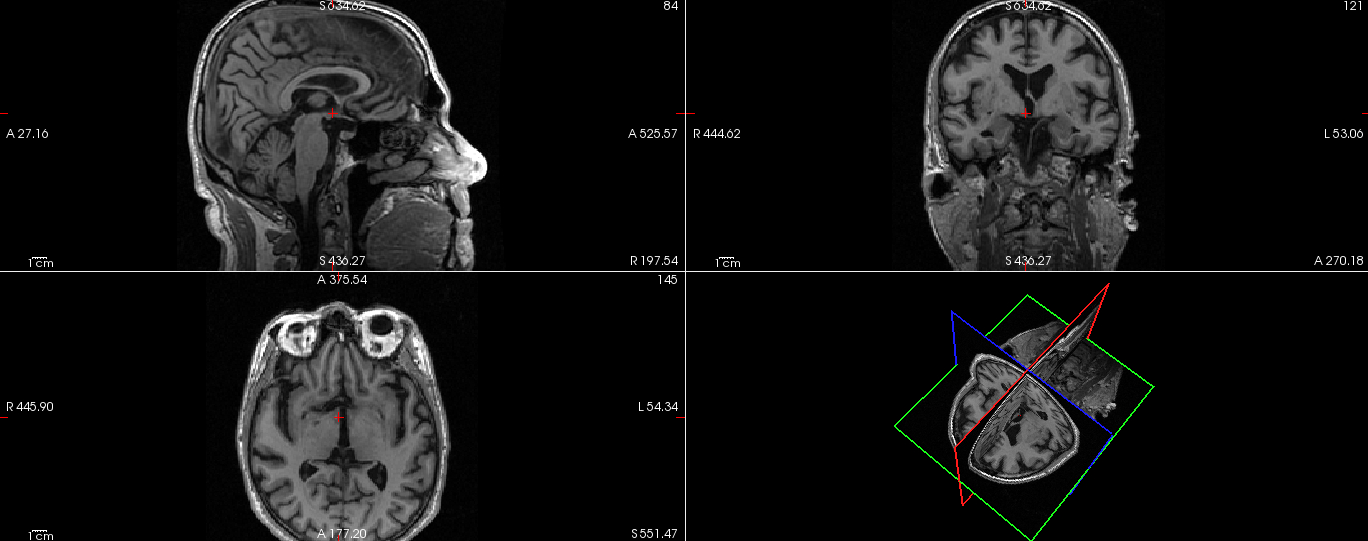
\includegraphics[width=0.95\linewidth]{mymans2}
	\caption{An example of the original raw image file, from subject 002\_S\_0295. This is the original raw image from the MRI scan and no processing has been done.}
	\label{fig:screenshot001}
\end{figure}

\subsubsection{Data Preprocessing}

In this project, the area of interest is the brain itself. A lot of different tools from the FreeSurfer Software Suite have been used to produce images of the brain. The constructed brain images and how to construct these for reproduction of the results will be described in the following. The raw image is called: \newline \texttt{
	% ADNI1\_baseline3T\_collection/002\_S\_0413/MPR\_\_\_\_N3\_\_Scaled\_2/2006-05-19\_16\_17\_47.0 /S14782/
ADNI\_002\_S\_0413\_MR\_MPR\_\_\_\_N3\_\_Scaled\_2\_Br\_20081001114937668\_S14782\_I118675.nii} and is shown in figure \ref{fig:screenshot001}. 
\\\\
The first thing that happens in the preprocessing is motion correction. If multiple images of the source volume has been taken, then correction for motion will be done by averaging all the images.
Next step in the preprocessing is non-parametric non-uniform intensity Normalization (N3), which corrects for intensity non-uniformity in the MRI image.
Then, the Talairach transformation is applied. This computes the affine transformation from the subject's original space into the MNI395 atlas.
Then, another normalization of the intensities in the original image is done. The intensity of all voxels are scaled so that the mean intensity of the white matter is 110 \cite{normalize}. 
As the brain is the key area of interest as mentioned earlier, the skull is stripped from the image. The skull-stripping process is done by using Freesurfer Software Suite and thresholding \cite{freesurfer}.
The FreeSurfer software will create files which can be used to check if too much brain matter is removed in the process of skull-stripping the raw image.
Files which can be used to inspect this include \texttt{brainmask.mgz, T1.mgz} and \texttt{brainmask.gcuts.mgz}.
Next, electromagnetic gaussian classifier array (EM-GCA) Registration is done which computes transforms to align
\texttt{mri/nu.mgz} to the default GCA atlas from the FreeSurfer Home folder. Lastly, the CA Normalization happens, which outputs a normalized version of the skull-stripped image. This is saved as \texttt{mri/norm.mgz} and is going to be used as the data for each subject in this project \cite{reckon}.
\\\\
All human brains are different and the raw images are recorded in one space for each subject.
In order to compare several brains, a registration of the images has to be done to ensure they are all in the same coordinate reference system (CRS). 
A standard CRS for the common brain is called the Talirach space. 
Each of the raw images in the ADNI-dataset are registered to the Talirach space using the \texttt{mni305.cor} template from FreeSurfer. 
This is done using \texttt{mri\_vol2vol}, which resamples a volume into another CRS. 
In this project, an MNI305 transformation has been applied by resampling the original normalized images into talairach space using \texttt{\$subject/mri/transforms/talairach.xfm} 

\subsubsection{Preprocessing Scripts}\label{preprocess_scripts}
%TODO: Det ville være federe at have i methods eller appendix måske
For this project, two different type of preprocessing scripts have been used. These will be shown in the appendix, but are a key importance of the project. The first script will apply the many preprocessing algorithms described in the previous section. Most importantly, it creates the \texttt{norm.mgz} image, which, as mentioned earlier, is a skull-stripped and normalized version of the subject's brain see code in figure \ref{script1} in appendix[\ref{appendix}].
The produced \texttt{norm.mgz} can be illustrated using Freeview, a FreeSurfer Software used to display and examine 3D images. 
When displaying the new \texttt{norm.mgz} file, a big difference can be seen between the image before processing in figure \ref{fig:screenshot001} and after processing in figure \ref{fig:norm}.

\begin{figure}[H]
	\centering
	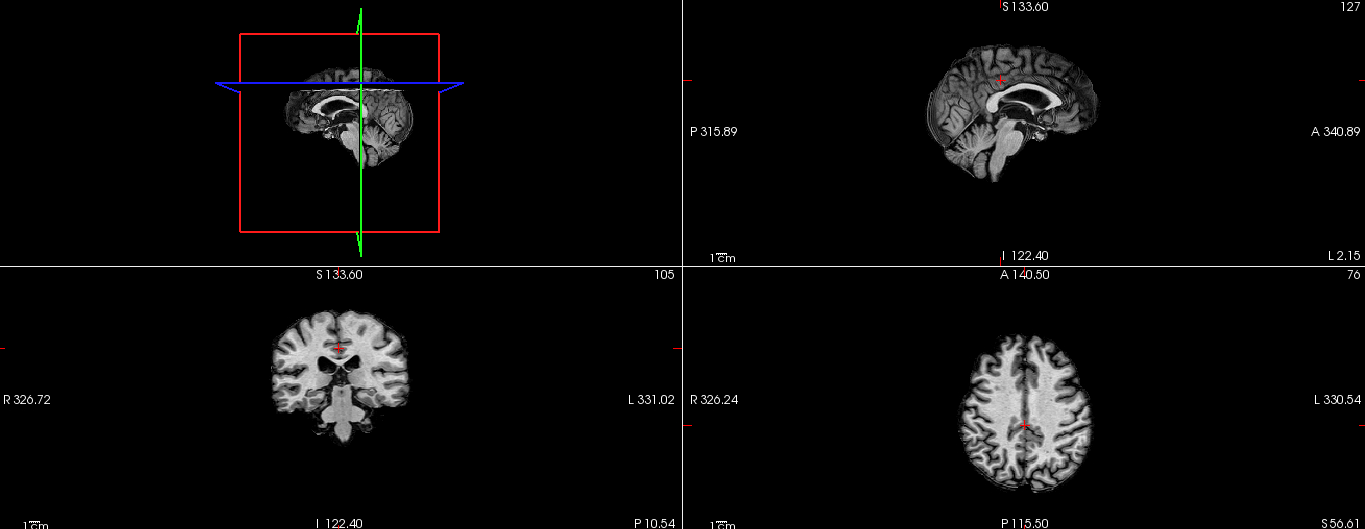
\includegraphics[width=0.9\linewidth]{imgs/norm}
	\caption{The above illustrates the \texttt{norm.mgz} for the subject \texttt{002\_S\_0295} in the subject's own normalized space.} 
	\label{fig:norm}
\end{figure}

The next script utilizes the \texttt{mri\_vol2vol} command, which uses advanced registration to ensure the \texttt{norm.mgz} image is in Talairach space using the mni305.cor.template - this will allow for both compatibility between the different subject images and opportunity to train a CycleGAN model to transfer between the two tesla domains. The script can be seen in the appendix, consult figure \ref{script2} in appendix[\ref{appendix}].
\noindent
The resulting image after the FreeSurfer preprocessing is shown in figure \ref{fig:norm305}. This image will resemble figure \ref{fig:norm}, but is in a different space, where it has been aligned to the MNI305 atlas. 

\begin{figure}[H]
	\centering
	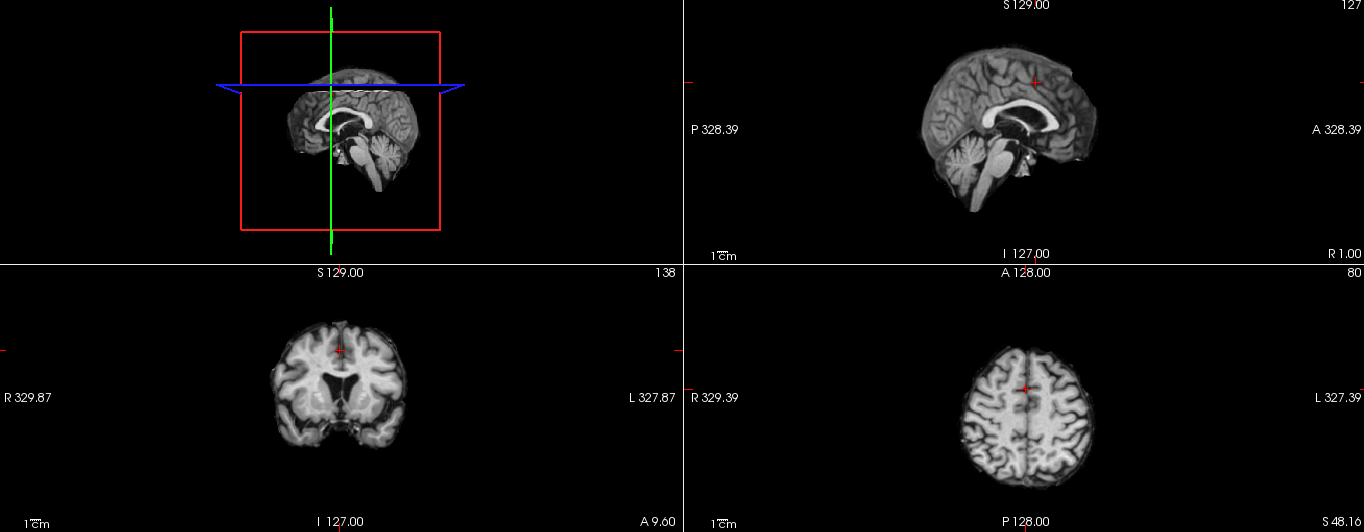
\includegraphics[width=0.9\linewidth]{imgs/norm_305}
	\caption{The \texttt{norm\_mni305.mgz} for the subject \texttt{002\_S\_0295} in the Talairach space.} 
	\label{fig:norm305}
\end{figure}


\subsection{Visualization of Data}
% Slices of img, preview 
This section aims to give a visualization of the preprocessed data. The section will illustrate the images used to train the CycleGANs in this project. The images are being constructed by thresholding one of the following dimension: $ x, y, z $ - which creates the following planes: \texttt{xy, xz, yz}. The xy-, xz- and yz-planes are 2D-images. If an image is converted to a \texttt{numpy nd} array, the slicing would amount to: \texttt{slice = np.array([:,:,z])}, where $ z \in [1,256] $. Thus, we have 256 2D images for each plane for every 3D image resulting in a total of $ 1.152 $ million 2D images. The training images are brain slices, which can be seen in the figures \ref{fig:slica_xy}, \ref{fig:slica_xz} and \ref{fig:slica_yz} \footnote{The images in figures are from randomly selected slices and do not match within 1.5T and 3T}. All the slices are created using the \texttt{create\_imgs\_1.5T.py} and \texttt{create\_imgs\_3T.py} python scripts which utilizes numpy and multiprocessing. The scripts can be seen in the repository of this project here: \href{https://github.com/oskarwiese/AlzPred/blob/main/preprocessing_scripts/slicing_scripts/3/create_imgs_3T.py}{3T\_script} and \href{https://github.com/oskarwiese/AlzPred/blob/main/preprocessing_scripts/slicing_scripts/1.5/create_imgs_1.5T.py}{1.5\_script}. %TODO: Path passer nok ikke længere
An important point to note is that completely black images are discarded. This means only slices with at least one pixel value different from zero are used to train the CycleGAN. This is partially a way to reduce the raw amount of training data, but it is also done because a CycleGAN would never need to learn to translate completely black images from 3T to 1.5T and vice versa, since the black slices can be removed from the image before conversion and reinserted afterwards.

\begin{figure}[H]
	\centering
	\begin{subfigure}[b]{0.7\textwidth}
		\centering
		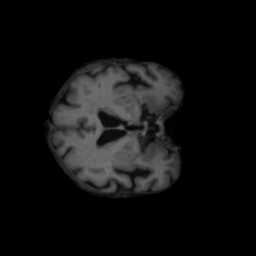
\includegraphics[width=0.475\linewidth]{imgs/xy_15T}%
		\hfill
		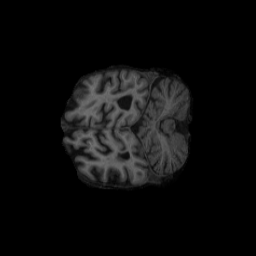
\includegraphics[width=0.475\linewidth]{imgs/xy_3T}
		\caption{1.5T (left) and 3T (right) respectively XY MRI Planes from subject 002\_S\_6695 and 009\_S\_4359}
		\label{fig:slica_xy}
	\end{subfigure}
		\vskip\baselineskip
	\begin{subfigure}[b]{0.7\textwidth}
		\centering
		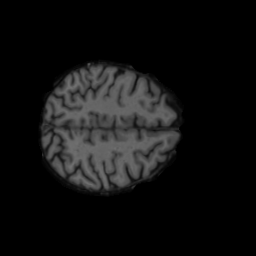
\includegraphics[width=0.475\linewidth]{imgs/002_S_0413_xz_1.5T}%
		\hfill
		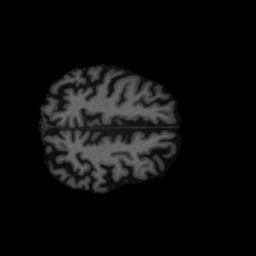
\includegraphics[width=0.475\linewidth]{imgs/002_S_4171_xz_3T}
		\caption{1.5T and 3T respectively XZ MRI Planes from subject 002\_S\_0413 and 002\_S\_4171}
		\label{fig:slica_xz}
	\end{subfigure}
	\vskip\baselineskip
	\begin{subfigure}[b]{0.7\textwidth}
		\centering
		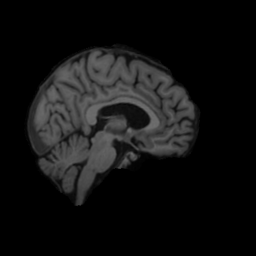
\includegraphics[width=0.475\linewidth]{imgs/002_S_0413_yz_15T}%
		\hfill
		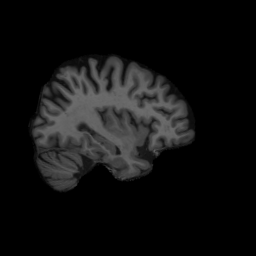
\includegraphics[width=0.475\linewidth]{imgs/002_S_4171_yz_3T}
		\caption{1.5T and 3T respectively YZ MRI Plane from subject 002\_S\_4171 and 002\_S\_0413.}
		\label{fig:slica_yz}
	\end{subfigure}
	\caption{Each of the subfigures show two examples from the three different planes constructed. The images displayed here is a part of the training data. }
\end{figure}

\subsubsection{Data Augmentation}
Besides the immense preprocessing done with the FreeSurfer Software Suite, the images are also resized, center cropped, converted to float and normalized with a $ \mu = 0.5 $ and $ \sigma = 0.5$. Centercrop crops an image in the center, ensuring that when the image is converted to a tensor and has an arbitrary number of leading dimensions, it will be cropped correctly. Furthermore, the intensity values are normalized to avoid the vanishing and exploding gradient problem when doing backpropagation.


\section{Methods}
%TODO: tror ikke alle subsections er nævnt her. Så vi skal nok endten nævne alle eller ingen 
This section introduces what technical background has been used in the duration of this project as well as which types of models have been trained. Section \ref{camillas_model} introduces the classification network used to find and analyze the bias present in using both 1.5T and 3T MRI images for analysis. Section \ref{gan} and \ref{cyclegan} consider the intuition and mathematical theory behind implementing GANs and CycleGANs. The GAN has been trained on the Modified National Institute of Standards and Technology database (MNIST) hand-drawn digit dataset as a preliminary introduction to GANs. The results of training this model is found in section \ref{MNIST_GAN}. As for the CycleGAN, five total models have been implemented on various datasets. One of these models was trained on the horse2zebra dataset used in the original CycleGAN paper \cite{original_cyclegan} as another preliminary experiment and as an introduction to CycleGANs. The result of this preliminary run is located in section \ref{horse2zebra_cyclegan}. The four other models have been trained on different variations of the MRI files mentioned above. One has been trained on slices from the $x$-axis (YZ), another from the $y$-axis (XZ), yet another on the $z$-axis (XY). The last model has been trained on all (ALL) of these images simultaneously and outputs and average 3D image from predicting each 3D image. The goal was to test the best approach for reconstructing 1.5T images from 3T images, and to see if the ALL-model could hold up to the quality of the other models. The specifics about training variables, hyperparameters, etc. are located in section \ref{model_specifics}. Since these models are not easy to train \cite{hard_to_train}, section \ref{troubleshooting} relays multiple issues along the training process and how they were eventually fixed. Lastly, section \ref{reproducibility} discusses what has been done to ensure reproducible results. %TODO: mangler sektioner. Kunne nok også godt gøres lidt kortere



\subsection{Generative Adversarial Network}\label{gan}
Since the meat and potatoes of this project is the CycleGAN, the methods and mathematical understanding behind GANs are important to grasp before diving deep into the theory of CycleGANs. A GAN was implemented on the MNIST dataset as a preliminary trail to help understand the basics. This implementation can be seen in the python script \texttt{train\_GAN.py}. An older version of the same code is also accessible as a Jupyter Notebook in our GitHub repository  \href{https://github.com/oskarwiese/AlzPred/blob/main/preliminary/GAN_MNIST.ipynb}{here}. This implementation in collaboration with this section will hopefully help to give the proper insight into the reasoning and intuition behind CycleGANs later in this section.

In general, GANs can be seen as two different complex neural networks competing for the best accuracy during  the process of generating a class of pictures. In other words, the networks are adversaries in generating or classifying images, from which the source of the name becomes clear. One of the networks will be focusing on generating fake images, called the \textit{generator}, and the other will be trying to distinguish between real and fake images, called the \textit{discriminator}. This competition between networks leads to results comparable or better than many ML and AI image generation techniques, thus making a good foundation for the generation of 1.5T MRI images from 3T. The two networks are covered in depth in the below subsections.
\begin{figure}[H]
	\centering
	\includegraphics[width=0.7\linewidth]{"imgs/GAN architecture"}
	\caption{The GAN architecture. The generator decodes random noise from a latent space into a fake image. This fake image as well as an image from the training set is fed into the Discriminator, which encodes data into a binary prediction of whether the image is real or fake. Figure courtesy of \cite{gan_introduction_towards_datascience}.}
	\label{fig:gan-architecture}
\end{figure}


\subsubsection{Generator}
The generator is the most important part of the GAN, since it is responsible for actually generating convincing images. Sadly, making a neural network generate real images is a difficult task to say the least. For that reason, instead of asking the generator to generate 28x28 hand-written digits by comparing the generator output to real digits using some objective function, the output of the generator is instead fed to the discriminator, which predicts if the generated image is real or not. If the discriminator is tricked by the generator, then the generator deserves a low loss for having made a "real" image (in practice, the generator and discriminator both start off unoptimized, so it takes many steps for real images to emerge). This is conceptually a much easier problem to solve, since the generator learns what is necessary to fool the discriminator instead of what characterizes a hand-written digit \cite{developers.google_generator}.

To generate the image, a \texttt{(batch\_size, 100)} vector of gaussian distributed noise is given as input, and the output is an image of dimension \texttt{(batch\_size, 1, 28, 28)}, since the image is black-white. The layers in-between consist of five linear layers. All layers but the last one have batch normalization and leaky-ReLU with $x$ set to $0.2$. The last layer uses hyperbolic tangent as activation function and is afterwards reshaped from $28^2$ to \texttt{(batch\_size, 1, 28, 28)} to be able to view the output as an image \cite{pathmind_gen_disc_architecture}. The architecture described above is also shown in table \ref{tab:gan_generator}.

\begin{table}[H]
	\centering
	\begin{tabular}{llll}\toprule
		Layer                        & Activation Size & Value & \# Parameters\\ \midrule
		Input                        & 100             &       & 0            \\
		linear layer                 & 2848            &       & 287,648      \\
		BatchNorm1d                  & 2848            & 2848  & 5,696        \\
		LeakyReLU                    & 2848            & 0.2   & 0            \\
		linear layer                 & 2848            &       & 8,113,952    \\
		BatchNorm1d                  & 2848            & 2848  & 5,696        \\
		LeakyReLU                    & 2848            & 0.2   & 0            \\
		linear layer                 & 2848            &       & 8,113,952    \\
		BatchNorm1d                  & 2848            & 2848  & 5,696        \\
		LeakyReLU                    & 2848            & 0.2   & 0            \\
		linear layer                 & 2848            &       & 8,113,952    \\
		BatchNorm1d                  & 2848            & 2848  & 5,696        \\
		LeakyReLU                    & 2848            & 0.2   & 0            \\
		linear layer                 & 28x28           &       & 2,233,616    \\
		Tanh                         & 28x28           & NA    & 0            \\
		                             &                 &       &              \\
		\textbf{Total Parameters}    &                 &       & 26,885,904   \\
		\textbf{Trainable Parameters}&                 &       & 26,885,904   \\  \bottomrule
	\end{tabular}
	\caption{All layers used in the final generator as well as how many parameters are used to train them. The activation size refers to the output of the layer in the same row. As such, applying the first linear layer yields an output vector of size $2848$. The input "layer" is added for completeness to show which size input is needed for the model to run correctly.}
	\label{tab:gan_generator}
\end{table}

The general flow of learning in the generator is as follows. First, random noise is fed to the generator as input. The generator uses this input to produce an image as output. This output is then fed to the discriminator as input. Afterwards, the discriminator outputs a prediction of whether the image is real or fake. The loss from this prediction is calculated and backpropagated through both models. This gives the gradients which are used only for updating the generator for better image generation in next step \cite{developers.google_generator}.

\subsubsection{Discriminator}
The discriminator is not nearly as important as the generator, though it still plays a very large role in generating likely images. If the discriminator did not do a good job predicting real images, the discriminator loss would not reflect accurately whether the generator did a good job creating plausible images. Thus, the generator would never converge towards a lower loss. This means that the discriminator has to improve at approximately the same rate as the generator \cite{developers.google_discriminator, developers.google_training}.

The discriminator, like any other classifier, can take as input whatever size and shape of data, as long as the architecture compensates for this change of data. For the case of predicting authenticity of MNIST hand-written digits, the entire \texttt{(batch\_size, 1, 28, 28)} image is given as input. As output, a \texttt{(batch\_size, 1)} vector is given. This vector is equivalent to the discriminator outputting a real or fake value for each image in the batch (0 being fake and 1 being real). The model contains six linear layers with an architecture made to be that of an autoencoder (see figure \ref{fig:autoencoder}). This means that the two first layers create deep features with lower dimension and the next four layers broaden the dimensions again while lowering the depth. Dropout with probability 0.15 is used to avoid overfitting and too fast learning, while leaky-ReLU is used for the first four layers. The sigmoid is used for the last layer to restrict the output values to be between 0 and 1, such that they mimic the probability of the input image being real \cite{pathmind_gen_disc_architecture}. The architecture of the discriminator model is visualized in table \ref{tab:gan_discriminator}.
\begin{table}[H]
	\centering
	\begin{tabular}{llll}\toprule
		Layer                        & Activation Size & Value & \# Parameters \\ \midrule
		Input                        & 28x28           &       & 0             \\
		linear layer                 & 32x32           &       & 803,840       \\
		Dropout                      & 32x32           & 0.15  & 0             \\
		LeakyReLU                    & 32x32           & 0.2   & 0             \\
		linear layer                 & 2048            &       & 2,099,200     \\
		Dropout                      & 2048            & 0.15  & 0             \\
		LeakyReLU                    & 2048            & 0.2   & 0             \\
		linear layer                 & 32x32           &       & 2,098,176     \\
		Dropout                      & 32x32           & 0.15  & 0             \\
		LeakyReLU                    & 32x32           & 0.2   & 0             \\
		linear layer                 & 512             &       & 524,800       \\
		Dropout                      & 512             & 0.15  & 0             \\
		LeakyReLU                    & 512             & 0.2   & 0             \\
		linear layer                 & 16x16           &       & 131,328       \\
		Dropout                      & 16x16           & 0.15  & 0             \\
		linear layer                 & 1               &       & 257           \\
		Sigmoid                      & 1               & NA    & 0             \\
		                             &                 &       &               \\
		\textbf{Total Parameters}    &                 &       & 5,657,601     \\
		\textbf{Trainable Parameters}&                 &       & 5,657,601     \\ \bottomrule
	\end{tabular}
	\caption{All layers used in the final generator and the number of needed parameters. For a detailed explanation, see table \protect\ref{tab:gan_generator}.}
	\label{tab:gan_discriminator}
\end{table}

Regarding the learning of the discriminator, one real and one fake image is first given as input. This gives the discriminator both positive and negative examples during training, which it tries to classify as real or fake. The discriminator performance is found using a loss function and this loss quantifies how well the discriminator predicted the validity of the images. This loss is high if the model classifies real images as fake or visa versa. Then, the discriminator weights are updated by backpropagating the loss thoughout the discriminator network. The generator weights are not updated in this step, as it needs to stay constant while generating examples of training images \cite{developers.google_discriminator, developers.google_training}.

\subsubsection{Loss}
For implementing the loss functions necessary to get a proper GAN going, we first need to define some nomenclature. We assume that sample images are sampled from $x \sim p_{\text {data}}(x)$. The discriminator $D(x)$ outputs a value between zero and one determining whether $x$ is real or fake. The generator takes random noise $z \sim p_{\text {data}}(z)$ and returns a fake sample. The loss function for the discriminator is given as shown below.

\[\begin{aligned}
	\mathcal{L}\left(G, D, X, Z\right)_D &=\frac{1}{2} \mathbb{E}_{x \sim p_{x}}[1-D(x)] \\
	&+\frac{1}{2} \mathbb{E}_{z \sim p_{z}}[D(G(z))] \\
\end{aligned}\]
Here, the first term simply forces the discriminator to try to return large values when the samples are real. As the discriminator output approaches 1, the loss approaches 0. The second term is slightly more complicated. The generated image $G(z)$ is given to the discriminator, and the goal of the discriminator is to catch that this is, in fact, a fake image. Thus, lower discriminator values on the fake image leads to lower loss and as the discriminator output approaches 0, this term of the loss also approaches 0.

Now for the generator loss, which is shown below.

\[\mathcal{L}\left(G, D, X, Z\right)_G=-1 \cdot \log \sigma\left(D(G(Z))\right)\]

This loss is equivalent to the binary cross-entropy (BCE) loss with logits, where the weights are all set to be equal. The $\sigma$ term is the sigmoid function. This loss function basically states that the generator gets a large loss when the discriminator gets tricked into thinking that the generated image is real. This is due to the fact that a low probability of it being a real image leads to a high loss and vica versa \cite{bcewithlogits}.


\subsection{CycleGAN}\label{cyclegan}
The GAN allowed for new images in a specific category to be created based on random noise. The next upgrade would be to be able to go from one category to another and back again. This is exactly the problem a CycleGAN aims to fix, which makes it perfect for this paper, since we aim to go from 3T images to 1.5T images. Going back is not as important in this case, but could prove useful for other purposes. The CycleGAN generally works by implementing two generator networks, each generating one category based on an image from the other category, and two discriminator networks, each predicting the probability of the input image actually being from the original category. This architecture is explained and showcased further in figure \ref{fig:cycleganarchitecture} and \ref{fig:cycleganarchitecture2} below.
% TODO: Vigtigt at komme ind på original paper

\subsubsection{General Model Architecture}
% Visualizer library (måske)
\begin{figure}[H]
	\centering
	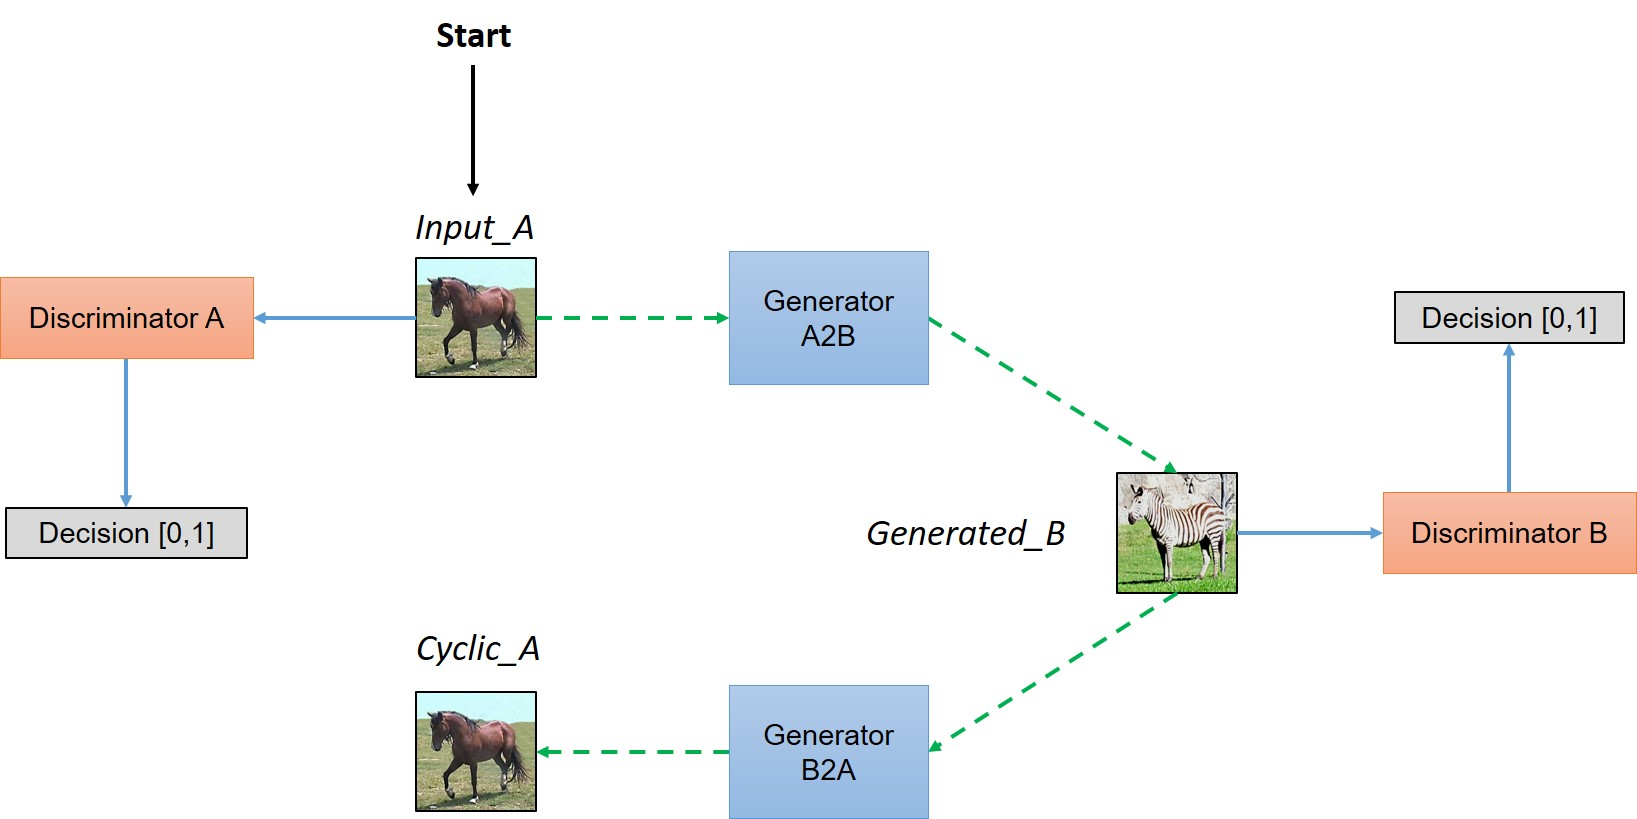
\includegraphics[width=0.7\linewidth]{imgs/cyclegan_architecture}
	\caption{This figure shows the interactions necessary for the four different networks to convert images from A to B. The input image of category A is fed directly to the discriminator and to the generator that converts images from A to B. This generates a fake image from category B, which is fed both to the discriminator to get a prediction and to the other generator to recover the image to one of category A for reasons that will become apparent later in this section. Figure courtesy of \cite{model_architecture}.}
	\label{fig:cycleganarchitecture}
\end{figure}

\begin{figure}[H]
	\centering
	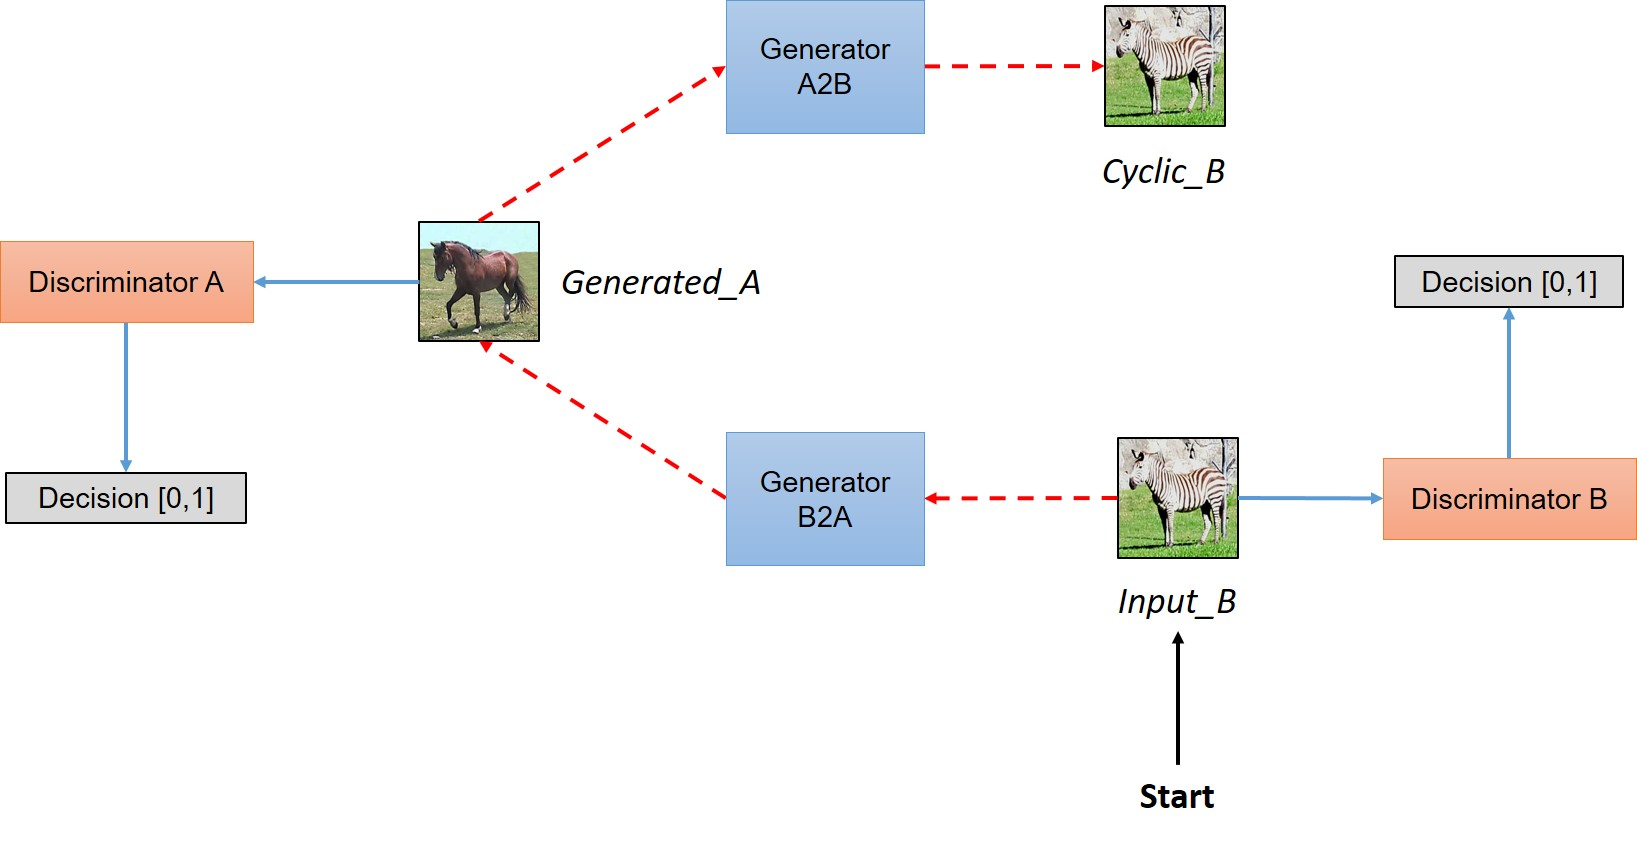
\includegraphics[width=0.7\linewidth]{imgs/cyclegan_architecture2}
	\caption{This figure is almost identical to figure \ref{fig:cycleganarchitecture}, although it shows the interactions necessary for the four different networks to convert images from B to A. For a basic explanation of the components involved, see the caption of figure \ref{fig:cycleganarchitecture}. Figure courtesy of \cite{model_architecture}.}
	\label{fig:cycleganarchitecture2}
\end{figure}


\subsubsection{Discriminator in a CycleGAN}
The discriminator of the model should take as input an image of size 1x256x256 (since the image is grayscale) and output a prediction of dimension 1x30x30 with values between zero and one. The reason the output is not just one value is because a patch-GAN is used. This move in dimensions is accomplished using up-sampling of the image with 2D-convolutions to extract increasingly abstract features by decreasing the height and width and increasing the depth of the image.

To make sure that the model is as robust as possible and to avoid overfitting, a patchGAN is used before outputting the final image prediction. This works by converting 30x30 blocks of the image into predictions, such that the model is forced to predict the validity of the image on each of these blocks. This ensures that the discriminator image can accurately predict if the image comes from the generator by using any part of the image. Some problems can occur with this method, like the model not being about to predict much from a 30x30 square of black pixels. These kinds of problems will be discovered further in the section \ref{discussion} on discussing problems with and efficacies of the model.

Of just as much importance as the patchGAN architecture and general model interactions is the layout of each layer and the functions used throughout the discriminator network. A general overview of the layers, kernel size, type of convolution, stride and padding is shown below in figure \ref{fig:cyclegandiscriminatorlayers}.
\begin{figure}[H]
	\centering
	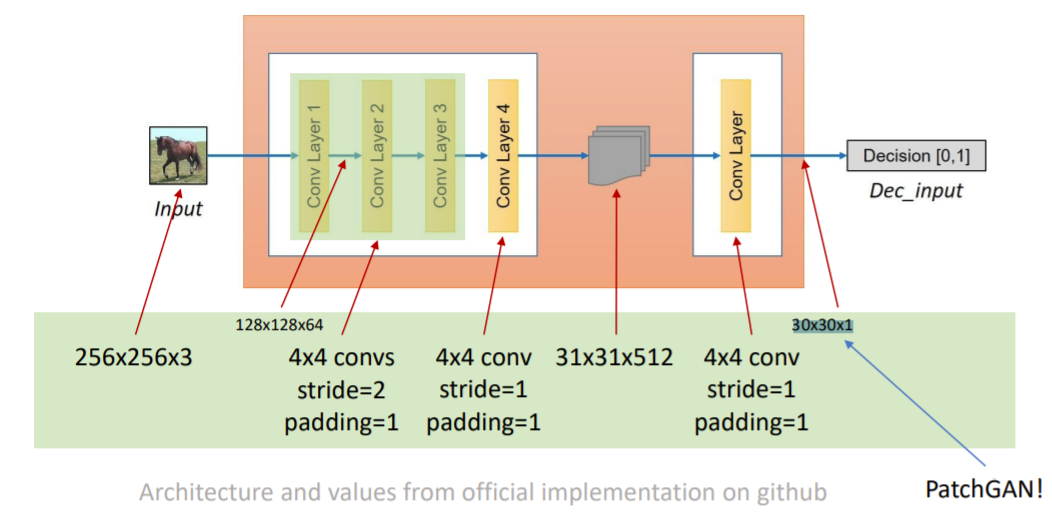
\includegraphics[width=0.7\linewidth]{imgs/cyclegan_discriminator_layers}
	\caption{The primary model layout consisting of the input, layers and output. The input is the gray-scale intensity-based MRI input of size 1x256x256. The five consecutive convolutional layers each have a specified kernel size, stride and padding as noted in the figure. The output is constructed from running the patchGAN on the last layer of the model to get a 1x30x30 matrix of values between 0 and 1. The specific values and layer sizes are specifed in table \ref{tab:discriminator_layers}. Figure courtesy of \cite{cyclegan_figures}.}
	\label{fig:cyclegandiscriminatorlayers}
\end{figure}

Not shown in the figure is the actions taken between each layer and the number of parameters used for each action. This can be seen below. 

\begin{table}[H]
	\centering
	\begin{tabular}{llll}\toprule
		Layer                         & Activation Size & Value & \# Parameters \\ \midrule
		Input                         & 3x256x256       &       & 0             \\
		64x4x4 conv, stride 2, pad 1  & 64x128x128      &       & 1,088         \\
		LeakyReLU                     & 64x128x128      & 0.2   & 0             \\
		128x4x4 conv, stride 2, pad 1 & 128x64x64       &       & 131,200       \\
		InstanceNorm2d                & 128x64x64       & 64    & 0             \\
		LeakyReLU                     & 128x64x64       & 0.2   & 0             \\
		256x4x4 conv, stride 2, pad 1 & 256x32x32       &       & 524,544       \\
		InstanceNorm2d                & 256x32x32       & 64    & 0             \\
		LeakyReLU                     & 256x32x32       & 0.2   & 0             \\
		512x4x4 conv, stride 1, pad 1 & 512x31x31       &       & 2,097,664     \\
		InstanceNorm2d                & 512x31x31       & 64    & 0             \\
		LeakyReLU                     & 512x31x31       & 0.2   & 0             \\
		1x4x4 conv, stride 1, pad 1   & 1x30x30         &       & 8,193         \\
		Sigmoid                       & 1x30x30         & NA    & 0             \\
		                              &                 &       &               \\
		\textbf{Total Parameters}     &                 &       & 2,762,689     \\
		\textbf{Trainable Parameters} &                 &       & 2,762,689     \\ \bottomrule
	\end{tabular}
	\caption{The convolutions, stride and padding of each layer in the discriminators. The values used in the activation functions and instance normalization as well as when they are used in the network have also been shown. The activation shape channels are equal to the output shape of each layer and the height and width are calculated using the formula from article \protect\cite{calculate_activation_shape}. For the convolutional layers, the convention in the "layer" column reads \texttt{output\_size x kernel\_height x kernel\_width}. The first layer thus outputs a vector with 64 channels after applying a convolution with a 4x4 kernel with a stride of 2 and padding of 1. Other details of how to read the table can be found in table \ref{tab:gan_generator}.}
	\label{tab:discriminator_layers}
\end{table}

\subsubsection{Generator in a CycleGAN}
Unlike in a standard GAN generator, where a random image from a latent space is used to create what ends up looking like a real image, the generators in the CycleGAN takes as input an image from one of the datasets. As such, the input dimension is 1x256x256 (since the image is grayscale). The output is of the exact same dimension, since the generator tries to generate an image from the opposite category using the input image. Between input and output, the general generator architecture is that of an autoencoder, as pictured below in figure \ref{fig:autoencoder}. The generator contains three layers in an encoder and a decoder, while 9 residual blocks reside between them. The encoder encodes features by narrowing the image dimensions down and widening the depth of the data. The decoder does exactly the opposite, extracting newfound information back into a new image. The residual blocks between the encoder and decoder serve the purpose of interpreting the encoded features. They also use skip connections, which provide an alternate path for the gradient. This helps the network reach convergence.

\begin{figure}[H]
	\centering
	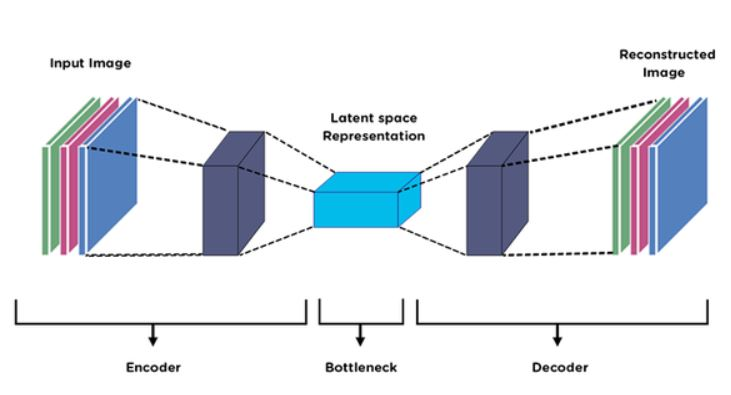
\includegraphics[width=0.7\linewidth]{imgs/autoencoder}
	\caption{The general autoencoder architecture. A kernel does convolutions to reduce and increase the image dimensions. The smaller the dimensions, the larger the feature complexity. The code between the encoder and decoder is referred to as residual blocks. These learn residual functions from the input of their last layer instead of learning unreferenced functions \cite{residual_blocks}. Figure courtesy of \cite{autoencoder}.}
	\label{fig:autoencoder}
\end{figure}


\begin{figure}[H]
	\centering
	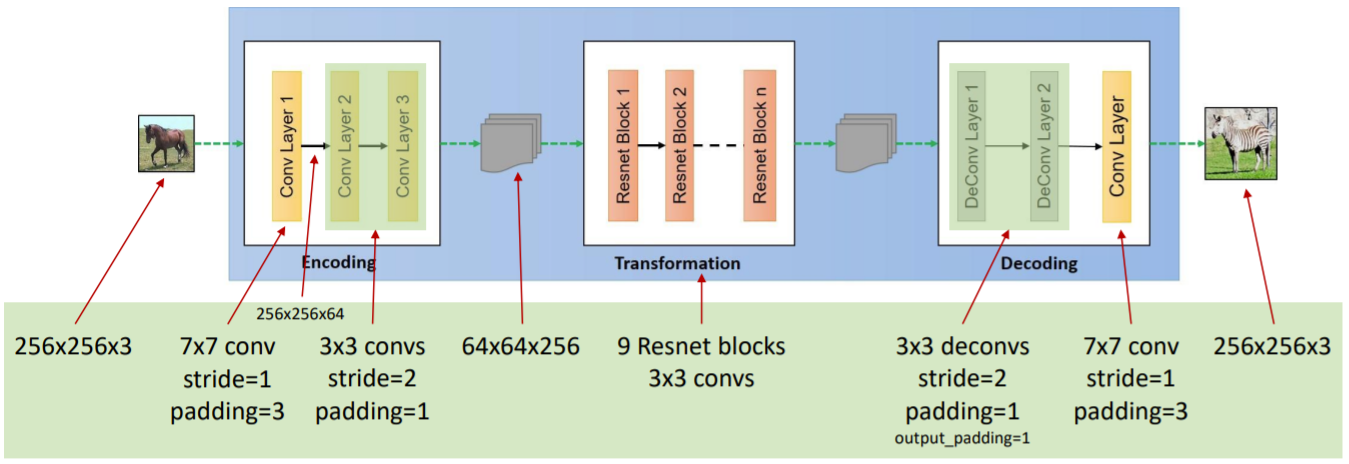
\includegraphics[width=0.7\linewidth]{imgs/cyclegan_generator_layers}
	\caption{The primary model layout consisting of the input, layers and output. The input is the gray-scale intensity-based MRI input of size 1x256x256. The five encoding and decoding convolutional layers as well as the residual blocks each have a specified kernel size, stride and padding as noted in the figure. The specific values and layer sizes are specifed in table \ref{tab:generator_layers}. Figure courtesy of \cite{cyclegan_figures}.}
	\label{fig:cyclegangeneratorlayers}
\end{figure}


%TODO: Explain components (norm and activation layers, convolutions, relu etc)
\begin{table}[H]
	\hspace*{-2cm}
	\begin{tabular}{llll}\toprule
		Layer                                       & Activation Size& Value       & \# Parameters \\ \midrule
		Input                                       & 3x256x256      &             & 0             \\
		64x6x6 conv, stride 1, pad 3                & 64x257x257     &             & 6,976         \\
		ReLU                                        & 64x257x257     & inplace=True& 0             \\
		128x3x3 conv, stride 2, pad 1               & 128x129x129    &             & 73,856        \\
		InstanceNorm2d                              & 128x129x129    & 128         & 0             \\
		ReLU                                        & 128x129x129    & inplace=True& 0             \\
		256x3x3 conv, stride 2, pad 1               & 256x65x65      &             & 295,168       \\
		InstanceNorm2d                              & 256x65x65      & 256         & 0             \\
		ReLU                                        & 256x65x65      & inplace=True& 0             \\
		9 residual blocks with relu and instancenorm& 256x65x65      &             & 10,621,440    \\
		Upsample                                    & 256x130x130    & 2,bilinear  & 0             \\   
		128x4x4 Conv2d stride 1, pad 2              & 128x131x131    &             & 524,416       \\
		InstanceNorm2d                              & 128x131x131    & 128         & 0             \\
		ReLU                                        & 128x131x131    & inplace=True& 0             \\
		Upsample                                    & 128x262x262    & 2,bilinear  & 0             \\   
		64x4x4 Conv2d stride 1, pad 1               & 64x261x261     &             & 131,136       \\
		InstanceNorm2d                              & 64x261x261     & 64          & 0             \\
		ReLU                                        & 64x261x261     & inplace=True& 0             \\
		3x8x8 conv, stride 1, pad 1                 & 3x256x256      &             & 12,291        \\
		Tanh                                        & 3x256x256      & NA          & 0             \\
		                                            &                &             &               \\
		\textbf{Total Parameters}                   &                &             & 11,665,283    \\
		\textbf{Trainable Parameters}               &                &             & 11,665,283    \\ \bottomrule
	\end{tabular}
	\caption{The convolutions, stride and padding of each layer in the generators. The values used in the activation functions and instance normalization as well as when they are used in the network have also been shown. Relevant details of how to read the table are found in the captions of tables \ref{tab:gan_generator} and \ref{tab:discriminator_layers}.}
	\label{tab:generator_layers}
\end{table}

\subsubsection{Objective Functions (Losses)}
For this section, a number of notations will be introduced. Since the goal is to map between the two domains $X$ and $Y$, we introduce $G : X \rightarrow Y$ and $F : Y \rightarrow X$. Furthermore, $y \sim p_{\text {data}}(y)$ and $x \sim p_{\text {data }}(x)$ refer to the distributions of each domain and $x$ and $y$ refer to samples from each domain. Lastly, the discriminators for each domain are given by $D_X$ and $D_Y$ \cite{original_cyclegan}.

This section will focus on how the objective functions are constructed to ensure the correct result from the discriminators and generators. In general, the losses are separated into three categories: adversarial losses, cycle-consistency losses and identity losses. 

Here, the adversarial losses aim to ensure that discriminators are able to distinguish between real and fake images and generators are able to generate convincing fake images. The cycle-consistency losses make sure that mapping an image through the two different generators one after the other will result in approximately the same image as the input. Lastly, the identity losses check that the generators do not augment images that are already part of the domain they map towards. More details on each of these losses can be seen in the rest of this section.

The final loss function, containing all the losses mentioned above, will look as shown below.

Our full objective is:
\[\begin{aligned}
	\mathcal{L}\left(G, F, D_{X}, D_{Y}\right) &=\mathcal{L}_{\mathrm{GAN}}\left(G, D_{Y}, X, Y\right) \\
	&+\mathcal{L}_{\mathrm{GAN}}\left(F, D_{X}, Y, X\right) \\
	&+\lambda_{cyc} \mathcal{L}_{\mathrm{cyc}}(G, F) \\
	&+\lambda_{iden} \mathcal{L}_{\mathrm{iden}}(G, F)
\end{aligned}\]

\noindent Here, $\mathcal{L}_{\mathrm{GAN}}\left(G, D_{Y}, X, Y\right)$ and $\mathcal{L}_{\mathrm{GAN}}\left(F, D_{X}, Y, X\right)$ are the adversarial losses for $G$ and $D_Y$ and $F$ and $D_X$ respectively. Meanwhile, $\mathcal{L}_{\mathrm{cyc}}(G, F)$ is the cyclic loss for both generators and $\mathcal{L}_{\mathrm{iden}}(G, F)$ is the identity loss for both generators. The values $\lambda_{cyc}$ and $\lambda_{iden}$ are hyperparameter weights, controlling the respective importance of each part of the total loss function.

The goal of the final loss function is now to have the generators $G$ and $F$ minimize the function and have the discriminators $D_X$ and $D_Y$ maximize the function. This leads to competition between the four models. This interplay can be seen below.

\begin{equation}\label{minimax}
	G^{*}, F^{*}=\arg \min _{G, F} \max _{D_{x}, D_{Y}} \mathcal{L}\left(G, F, D_{X}, D_{Y}\right).
\end{equation}

The adversarial losses, shown below, are principally the simplest of the losses to understand. They simply make sure that the discriminators are very sure that real images are real and fake images are fake, while the generator becomes increasingly better at fooling the discriminator (creating convincing fake images). Modeling this behavior into an equation is simple, since the discriminator $D_Y$ approaches minimal adversarial loss as it gets closer to predicting 1 for real images and 0 for generated images. Meanwhile, the opposite is true for the generator. Since the discriminators want to maximize the below equations and the generators want to minimize them, these models have an antagonistic relationship and constantly need to sacrifice the performance of the other model to get better performance itself. This has been shown countless times in the literature to be fruitful and is the basis of GAN-based techniques.

\[\begin{aligned}
	\mathcal{L}_{\mathrm{GAN}}\left(G, D_{Y}, X, Y\right) &=\mathbb{E}_{y \sim p_{\text {data }}(y)}\left[\log D_{Y}(y)\right] \\
	&+\mathbb{E}_{x \sim p_{\text {data }}(x)}\left[\log \left(1-D_{Y}(G(x))\right],\right.
\end{aligned}\]

\[\begin{aligned}
	\mathcal{L}_{\mathrm{GAN}}\left(F, D_{X}, X, Y\right) &=\mathbb{E}_{x \sim p_{\text {data }}(x)}\left[\log D_{X}(x)\right] \\
	&+\mathbb{E}_{y \sim p_{\text {data }}(y)}\left[\log \left(1-D_{X}(F(y))\right],\right.
\end{aligned}\]

It turns out that the above adversarial losses are not always strenuous enough to map the input $x_i$ to an output $y_i$. Therefore, another set of loss functions are added; the forward and backward cycle-consistency loss functions, shown under this paragraph. The goal of these functions is to make sure that an image from $X$ mapped to $Y$ and mapped back to $X$ again will closely resemble the original image. That is, $x \rightarrow G(x) \rightarrow F(G(x)) \approx x$.This concept is called forward cycle-consistency loss, while the same is true for the other direction, backward cycle-consistency loss: $y \rightarrow F(y) \rightarrow G(F(y)) \approx y$. As can be seen in the two equations below, the L1-loss is taken between the original image $x$ and the double-generated image $F(G(x))$. The generators $G$ and $F$ then aim to minimize these terms, such that the two images are as closely resembling as possible. This loss is focused on the generators specifically, since the discriminators only play a roll in predicting if the image is real.

\[\begin{aligned}
	\mathcal{L}_{\text {cyc }}(G, F) &=\mathbb{E}_{x \sim p_{\text {data }}(x)}\left[\|F(G(x))-x\|_{1}\right] \\
	&+\mathbb{E}_{y \sim p_{\text {dau }}(y)}\left[\|G(F(y))-y\|_{1}\right] .
\end{aligned}\]

The identity loss formulated below punishes the model if the generator changes an image that is already part of the domain it transforms to. That is, $y_{new} = G(y)$ gets zero identity loss if $y_{new}$ and $y$ are completely identical and high loss if there are vast differences. The identity loss usually keeps the generators from changing the colors of the input image to get lower errors.

\[\begin{aligned}
	\mathcal{L}_{\text {iden }}(G, F) &=\mathbb{E}_{x \sim p_{\text {data }}(x)}\left[\|F(y)-x\|_{1}\right] \\
	&+\mathbb{E}_{y \sim p_{\text {data }}(y)}\left[\|G(x)-y\|_{1}\right] .
\end{aligned}\]


\subsubsection{Optimizer, Cross Entropy, Etc.}
A table of the used hyperparameters and their values in this project in given below. Note that these hyperparameters are applied to different models. Kernel size, stride and padding for each of the convolutional layers of the discriminator and generator are shown in tables \ref{tab:gan_generator}, \ref{tab:gan_discriminator}, \ref{tab:discriminator_layers} and \ref{tab:generator_layers}.
\begin{table}[H]
	\centering
	\begin{tabular}{l l l l l l l l l}
		\toprule
		& \textbf{Hyperparameter}     &&&&& & \textbf{Value}   & \\ \midrule
		& \multicolumn{7}{c}{\textbf{General}}              & \\
		& Batch size                  &&&&& & $1$           & \\
		& $\lambda_{iden}$            &&&&& & $1$           & \\
		& $\lambda_{cyc}$             &&&&& & $10$          & \\
		& Optimizer                   &&&&& & Adam          & \\
		& Betas                       &&&&& & $(0.5, 0.999)$& \\
		&                             &&&&& &               & \\
		& \multicolumn{7}{c}{Discriminator}                 & \\
		& input dimension             &&&&& & $1x256x256$   & \\
		& Conv depths                 &&&&& & $\left[3, 64, 128, 256, 512\right]$& \\
		& Output dimension            &&&&& & $1x30x30$     & \\
		& Leaky-ReLU activation       &&&&& & $0.2$         & \\
		&                             &&&&& &               & \\
		& \multicolumn{7}{c}{Generator}                     & \\
		& Input dimension             &&&&& & $1x256x256$   & \\
		& Conv depths                 &&&&& & $\left[64, 128, 256, 128, 64\right]$              & \\
		& Output dimension            &&&&& & $1x256x256$   & \\
		&                             &&&&& &               & \\ 
		& \multicolumn{7}{c}{\textbf{XY Model}}             & \\
		& Discriminator learning rate &&&&& & $5e-8$        & \\
		& Generator learning rate     &&&&& & $1e-7$        & \\
		& Number of epochs            &&&&& & $1.5$         & \\
		& Number of steps             &&&&& & $240000$      & \\
		&                             &&&&& &               & \\
		& \multicolumn{7}{c}{\textbf{XZ Model}}             & \\
		& Discriminator learning rate &&&&& & $5e-8$        & \\
		& Generator learning rate     &&&&& & $1e-7$        & \\
		& Number of epochs            &&&&& & $2$           & \\
		& Number of steps             &&&&& & $265000$      & \\
		&                             &&&&& &               & \\
		& \multicolumn{7}{c}{\textbf{YZ Model}}             & \\
		& Discriminator learning rate &&&&& & $1e-7$        & \\
		& Generator learning rate     &&&&& & $1e-7$        & \\
		& Number of epochs            &&&&& & $1.4$         & \\
		& Number of steps             &&&&& & $176000$      & \\
		&                             &&&&& &               & \\
		& \multicolumn{7}{c}{\textbf{ALL Model}}            & \\
		& Discriminator learning rate &&&&& & $7e-8$        & \\
		& Generator learning rate     &&&&& & $1e-7$        & \\
		& Number of epochs            &&&&& & $0.5$         & \\		
		& Number of steps             &&&&& & $245000$      & \\
		\bottomrule
	\end{tabular}
\end{table} 
The optimizer, batch size, betas, convolution depths and input/output were set to the same value as in the original CycleGAN paper, as this turned out to be efficacious on ADNI images too. Most notably, the number of epochs has been drastically reduced (from 200 in the original paper to under two in most of the models). This is due to the fact that the training data used in this project is much more plentiful than originally used to train the first CycleGAN in the paper. This means that we can get away with using vastly fewer epochs, since we still get the same number of overall steps. The weight $\lambda_{iden}$ was set to 1 in this project, since it gave better performance than the 0 value from the CycleGAN paper.

In relation to the discriminator and generator convolution depths, it is self-explanatory that using other images (RGB, non-square, different dimension) would require changing the architecture of input and output dimensions of all four models while also ensuring that the kernel size, stride and padding of the convolutional layers are setup correctly. This can be double checked by using $output\_dim = n - k + p + 1$, where $n$ is the image dimension, $k$ is kernel size and $p$ is padding.


\subsubsection{Troubleshooting}\label{troubleshooting}
Since implementing a CycleGAN requires implementing four different neural networks, the hyperparameter search and minutia of the model can be difficult to get right. Many issues like non-convergence, mode collapse, diminished gradients, vanishing gradients and more are well documented \cite{hard_to_train}. A known problem is CycleGAN only training until they reach a local minimum \cite{ganlocalminimum}. Another is the issue of getting noisy squares in images, sometimes referred to as checkerboard noise. One of the first models that was trained on the MRI ADNI images turned out to contain a version of this checkerboard noise. The source of noise turned out to be an uneven sampling of pixels in earlier layers to newer layers when doing the upsampling (also known as transpose convolution or deconvolution). Mismatches between the kernel size and the stride as well as bad upscaling can cause some areas of the upsampled image to contain information from more pixels than other areas. This is a critical cause of the recognizable checkerboard noise \cite{checkerboard}. An illustration of how the flaw gets made can be seen below. images generated from the flawed CycleGAN can also be seen in illustration \ref{fig:troubleshoota}. Here, it is clear that white squares are surrounded by black squares all over the image, worsening the general image quality.

\begin{figure}[H]
	\centering
	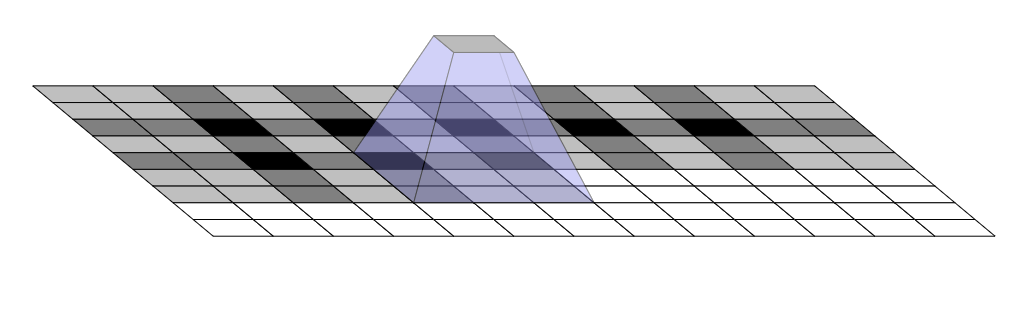
\includegraphics[width=0.7\linewidth]{imgs/deconvolution_mismatch}
	\caption{When the kernel size is not divisible by the stride, the image gets higher intensity in some areas than others leading to a checkerboard pattern. Shown here is a deconvolution using kernel size of 3 and stride of 2. Figure courtesy of \cite{checkerboard}.}
	\label{fig:deconvolutionmismatch}
\end{figure}
Solving this problem in practice first required separating upsampling from convolution. This works since the more intensity between pixels is split between multiple pixels. Doing this in practice involved switching every deconvolution layer except the last one from \texttt{nn.ConvTranspose2d(in\_channels, out\_channels, **kwargs)} to first \texttt{nn.Upsample(scale\_factor=2, mode='bilinear', align\_corners=True)} and then \texttt{nn.Conv2d(in\_channels, out\_channels, **kwargs)}. In a nutshell, instead of running a transpose convolution, an upsampling is perform to double the size of the image using bilinear interpolation and then a standard convolution is performed. This not only solves most of the checkerboard issues but also ensures that the model is able to learn from the decoding, since (\texttt{nn.Conv2d} and \texttt{nn.ConvTranspose2d} have trainable kernels while \texttt{nn.Upsample} does not) \cite{learnableKernel}. After implementing this functionality, the generated images now look like shown in illustration \ref{fig:troubleshootb}. We now see that most of the checkerboard artifacts are gone, though some vertical and horizontal lines still persist. A weird white void has also been generated around about half of the images for some reason.

The slight lines in the generated images after using bilinear interpolation for upsampling are not nearly as problematic but are still unfortunate as a final output. To solve this, we implemented a kernel size that was divisible by the stride in the deconvolution layers, as was mentioned as a solution in the previous paragraph. This should make the kernel spread information from each pixel more evenly between new pixels and supply a less grainy final image \cite{checkerboard}. In illustration \ref{fig:troubleshootc}, most of the noise has finally been removed and no lines persist in the image. The white voids around the brain seems to have become even more prevalent though, which also needs to be fixed. This was taken care of by replacing bilinear interpolation with nearest-neighbor interpolation. The result of replacing the interpolation can be seen in \ref{fig:troubleshootd}. It is now evident that basically no noise is left in the image, and most of the troubleshooting relating to image quality has thus subsided. The full comparison between results after each improvement has been implemented, can be seen in figure \ref{fig:troubleshoot}.

\begin{figure}[H]
	\centering
	\begin{subfigure}[b]{0.7\textwidth}
		\centering
		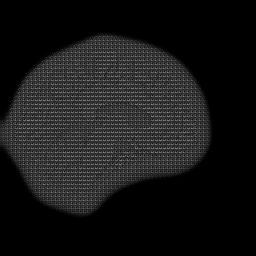
\includegraphics[width=0.475\linewidth]{imgs/1.5T_MRI_artifact}%
		\hfill
		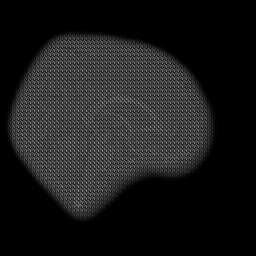
\includegraphics[width=0.475\linewidth]{imgs/3T_MRI_artifact}
		\caption{1.5T and 3T respectively YZ MRI images from the preliminary run.}
		\label{fig:troubleshoota}
	\end{subfigure}
	\vskip\baselineskip
	\begin{subfigure}[b]{0.7\textwidth}
		\centering
		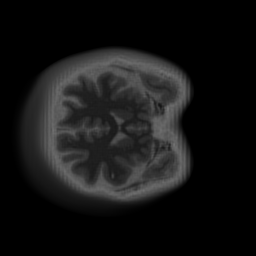
\includegraphics[width=0.475\linewidth]{imgs/vertical_noise_example}%
		\hfill
		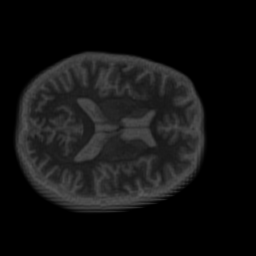
\includegraphics[width=0.475\linewidth]{imgs/horizontal_noise_example}
		\caption{1.5T and 3T respectively YZ MRI images after bilinear interpolation has been implemented in upsampling.}
		\label{fig:troubleshootb}
	\end{subfigure}
	\vskip\baselineskip
\end{figure}
\begin{figure}[H]
	\centering
	\begin{subfigure}[b]{0.7\textwidth}
		\centering
		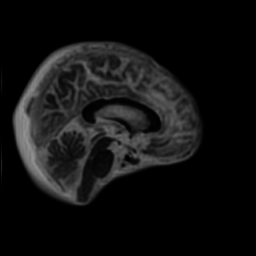
\includegraphics[width=0.475\linewidth]{imgs/1.5T_bilinear}%
		\hfill
		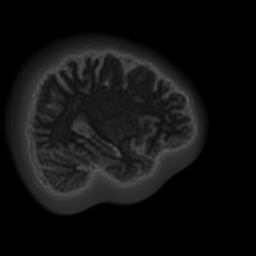
\includegraphics[width=0.475\linewidth]{imgs/3T_bilinear}
		\caption{1.5T and 3T respectively YZ MRI images after making kernel size divisible by stride.}
		\label{fig:troubleshootc}
	\end{subfigure}
	\begin{subfigure}[b]{0.7\textwidth}
		\centering
		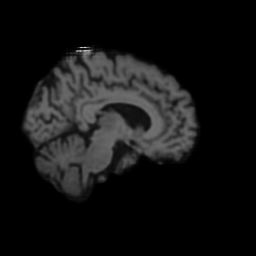
\includegraphics[width=0.475\linewidth]{imgs/1.5T_no_noise}
		\hfill
		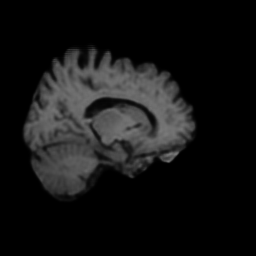
\includegraphics[width=0.475\linewidth]{imgs/3T_no_noise}
		\caption{1.5T and 3T respectively YZ MRI images after bilinear interpolation has been changed to nearest neighbor interpolation.}
		\label{fig:troubleshootd}
	\end{subfigure}
	\caption{Comparison of troubleshooting efforts to solve the visual issues in the generated images from the generators.}
	\label{fig:troubleshoot}
\end{figure}
Even after the struggle of implementing all of the these changes, some challenges are still present when generating images, though at this point the severity of the problems has been significantly reduced. It turns out that very rarely, images that are converted from $3T$ to $1.5T$ get a coupe horizontal white lines in the top of the image. This artifact can be seen in figure \ref{fig:troubleshoot_horizontals} for a random subject for each field-strength, where the above explained case manifested itself. This artifact seemed to be so rare that it was deemed unimportant to fix in this project.

\begin{figure}[H]
	\centering
	\begin{subfigure}[b]{0.7\textwidth}
		\centering
		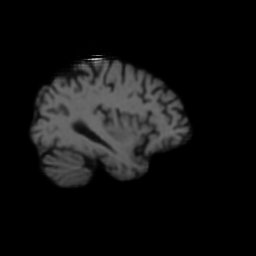
\includegraphics[width=0.475\linewidth]{imgs/1.5T_hori1}%
		\hfill
		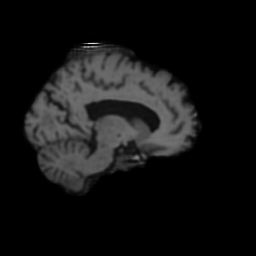
\includegraphics[width=0.475\linewidth]{imgs/1.5T_hori2}
	\end{subfigure}
	\caption{Two generated images before training was completed (half an epoch and one and a half epochs respectively). The left image is 1.5T and the right is 3T. The image artifact occurs only on the top of the $1.5T$ images, where a trading pattern of low-intensity and high-intensity pixels can be seen forming small horizontal lines.}
	\label{fig:troubleshoot_horizontals}
\end{figure}
Another issue entirely turned out to be that the vast number of input images all mapped to the same output image. This problem is well-known and is commonly called mode collapse. Figuring out that the models suffered from mode collapse normally required either plotting loss curves and seeing oscillations in the generator loss or sampling a number of images using different input images. In the generator models from this paper, no signs of mode collapse could be seen in the loss curves except for the discriminator constantly having very low loss. It was very evident that the generator only created one image when given multiple input images though \cite{mode_collapse_MLM}.

Many solution to the problem of mode collapse exist, some being much easier to implement than other. Easier solutions include reducing the learning rate, making separate learning rates for the discriminators and generators and only updating the discriminator if the accuracy of the discriminator in the current step is under 50\%. Harder solutions include implementing instance noise, making the generator better or making the discriminator worse. For the discriminators in this project, it turned out that it was enough to implement the accuracy check before updating the discriminators, reducing the learning rate and making separate learning rates for generators and discriminators. The others methods have been left in this section for future reference \cite{mode_collapse_reddit_fix}\cite{mode_collapse_github}. After implementing these fixes, the model was able to generate output samples from a much larger distribution, which indicates that the mode collapse has been fixed. A number of generated images can be seen in section \ref{results}.


\subsection{CycleGAN Evaluation Metrics}\label{evaluation_metrics}
To be able to properly evaluate whether the CycleGAN models have learned to effectively move between 1.5T and 3T images, a number of evaluation metrics have been applied. This section will explain the background behind these as well as what is expected for bad and good performance when using each metric.

\subsubsection{Visual Inspection}\label{visual_inspection}
The first evaluation metric, visual inspection, is also the most obvious one. By showing the generated images in a figure next to the ground truth, it is possible to firstly evaluate if the generated image even looks like a brain and secondly if the generated image looks like the brain it is supposed to be mapping towards. This seemingly simple metric might be the most important one, since the first step toward generating convincing brains is to make them look convincing to humans.

\subsubsection{image Subtraction}\label{image_subtraction}
A second visual way to visually inspect the images is to subtract images from each other and look at the resulting edge images. This allows for inspection of where the two images either agree or do not agree. In this report, image subtraction has been used between the 1.5T ground truth and 3T ground truth images as well as between the 1.5T ground truth and 1.5T generated images. This allows for comparison between how well the 1.5T generated image and the 3T ground truth images fit onto the 1.5T ground truth image. Images that are closer to matching will have fewer high-intensity pixels and a generally darker image. The hope is thus that the subtracted image containing the generated image has lower intensity than the ground truth image.

\subsubsection{Root-Mean-Square Error}\label{rmse}
Another way to show how closely the generated image matches the real one is to calculate the root-mean-square error between every pixel in the two images. This is done by applying
\begin{equation}
	RMSE = \sqrt{\frac{1}{n}\Sigma_{i=1}^{n}{\Big(y_i - \hat{y}_i\Big)^2}}\cite{sklearn.metrics.root_mean_square_error}
\end{equation}
where $n$ is the total number of pixels, $y_i$ is the real image and $\hat{y}_i$ is the fake image. Only calculating this value for one set of images would not give much info, so instead, RMSE has been found for two sets of images. Between the two 1.5T ground truth and 3T ground truth images and between the 1.5T ground truth and 1.5T generated images. This allows for an easy method of comparison, since a smaller difference between the generated and ground truth image than between the ground truth set would mean that the model has, to some extent, learned to replicate the patterns seen in 1.5T images.

\subsubsection{Geometric Accuracy}\label{geometric_accuracy}
The geometric accuracy, like the root-mean-square error, is another more precise metric for determining how close two image are to matching. As an accuracy measure, this method calculates how high a percentage of two images contain the same pixel by doing a pixel-wise comparison.

\begin{equation}
	\textrm{Geometric accuracy} = \frac{\Sigma_{i=1}^{n}\mathds{1}}{n}, \qquad
	  \mathds{1}=\begin{cases} 1, & \text{if $y_i = \hat{y}_i$}.\\ 0, & \text{otherwise}.\end{cases}
\end{equation}
Here, $n$ is the total number of pixels that will be compared in the image. This accuracy measure accomplishes much the same as other accuracy measures in that it show how often the model gets a pixel exactly right. As such, a higher accuracy means that the model is more successful in creating the real 1.5T image. It is only possible to calculate this metric on the image data because the values have been rounded to \texttt{uint8} integer values. Otherwise the pixel values would never be equal and the accuracy would be 0.


\subsection{Classifier}

In order to investigate whether a CycleGAN can be used to remove bias from a classifier, this project will introduce a Convolutional Neural Network (CNN), inspired heavily by Basai et al. and Camilla Kergel \cite{CamillaKandidat} \cite{neuro}. This section will present the architecture of the CNN, the applied hyperparameters as well as some highlighted differences from the other papers.

\subsubsection{Neural Network for Alzheimer's Disease Classification} \label{camillas_model}
In recent work with Alzheimer's disease classification by Camilla, a neural network was trained to predict whether patients had AD and the largest biases were found. Since the largest bias found in the model was between 1.5T and 3T images, a similar model was used to compare and contrast if the above described methods succeeded in removing the most prominent biases from the model, namely, the difference between 1.5T and 3T images. The model was implemented as a PyTorch neural network with 6 convolution layers using ReLU as activation function between each layer. This was followed by a fully connected layer with sigmoid activation to output the probability of each class (sick or healthy).  \cite{CamillaKandidat}.

\subsubsection{Data}
The data used for training the classifier is a combination of generated images from a CycleGAN\footnote{Important to note that only the CycleGAN trained on xy plane is used to generate the images used for training the classifier. This will be touched upon again in the discussion, see section \ref{future_work_mult}.} model as well as the original data from ADNI, which has been described in section \ref{dataDescription}. By training a classifier on the data, it was tested whether the model would inherit a bias towards the generated images. The goal was to prove that this bias does not exist by using dimensionality reduction algorithms on the penultimate linear layer from the model. There were 939 images in the training data and 235 in the test data. However, augmentation was used to create a more robust model. Three types of augmentations happened randomly with a probability, $ p = 0.8 $. The augmentations used were a random rotation, random flip or a random elastic deformation. The goal of using augmentation was to both create more training data and ensure a robust and generalization model after training. 

\subsubsection{Deep Neural Network Model}

	The implemented network is a convolutional neural network (CNN) which is a special type of deep neural network. The name stems from the most important operation in the network which is convolutions. In short, a convolution is the process of convolving a kernel with the image. An example of convolutions and a simple step in the convolution between an image named input and a horizontal Sobel filter can be seen in figure \ref{fig:convolution}.
	
	\begin{figure}[H]
		\centering
		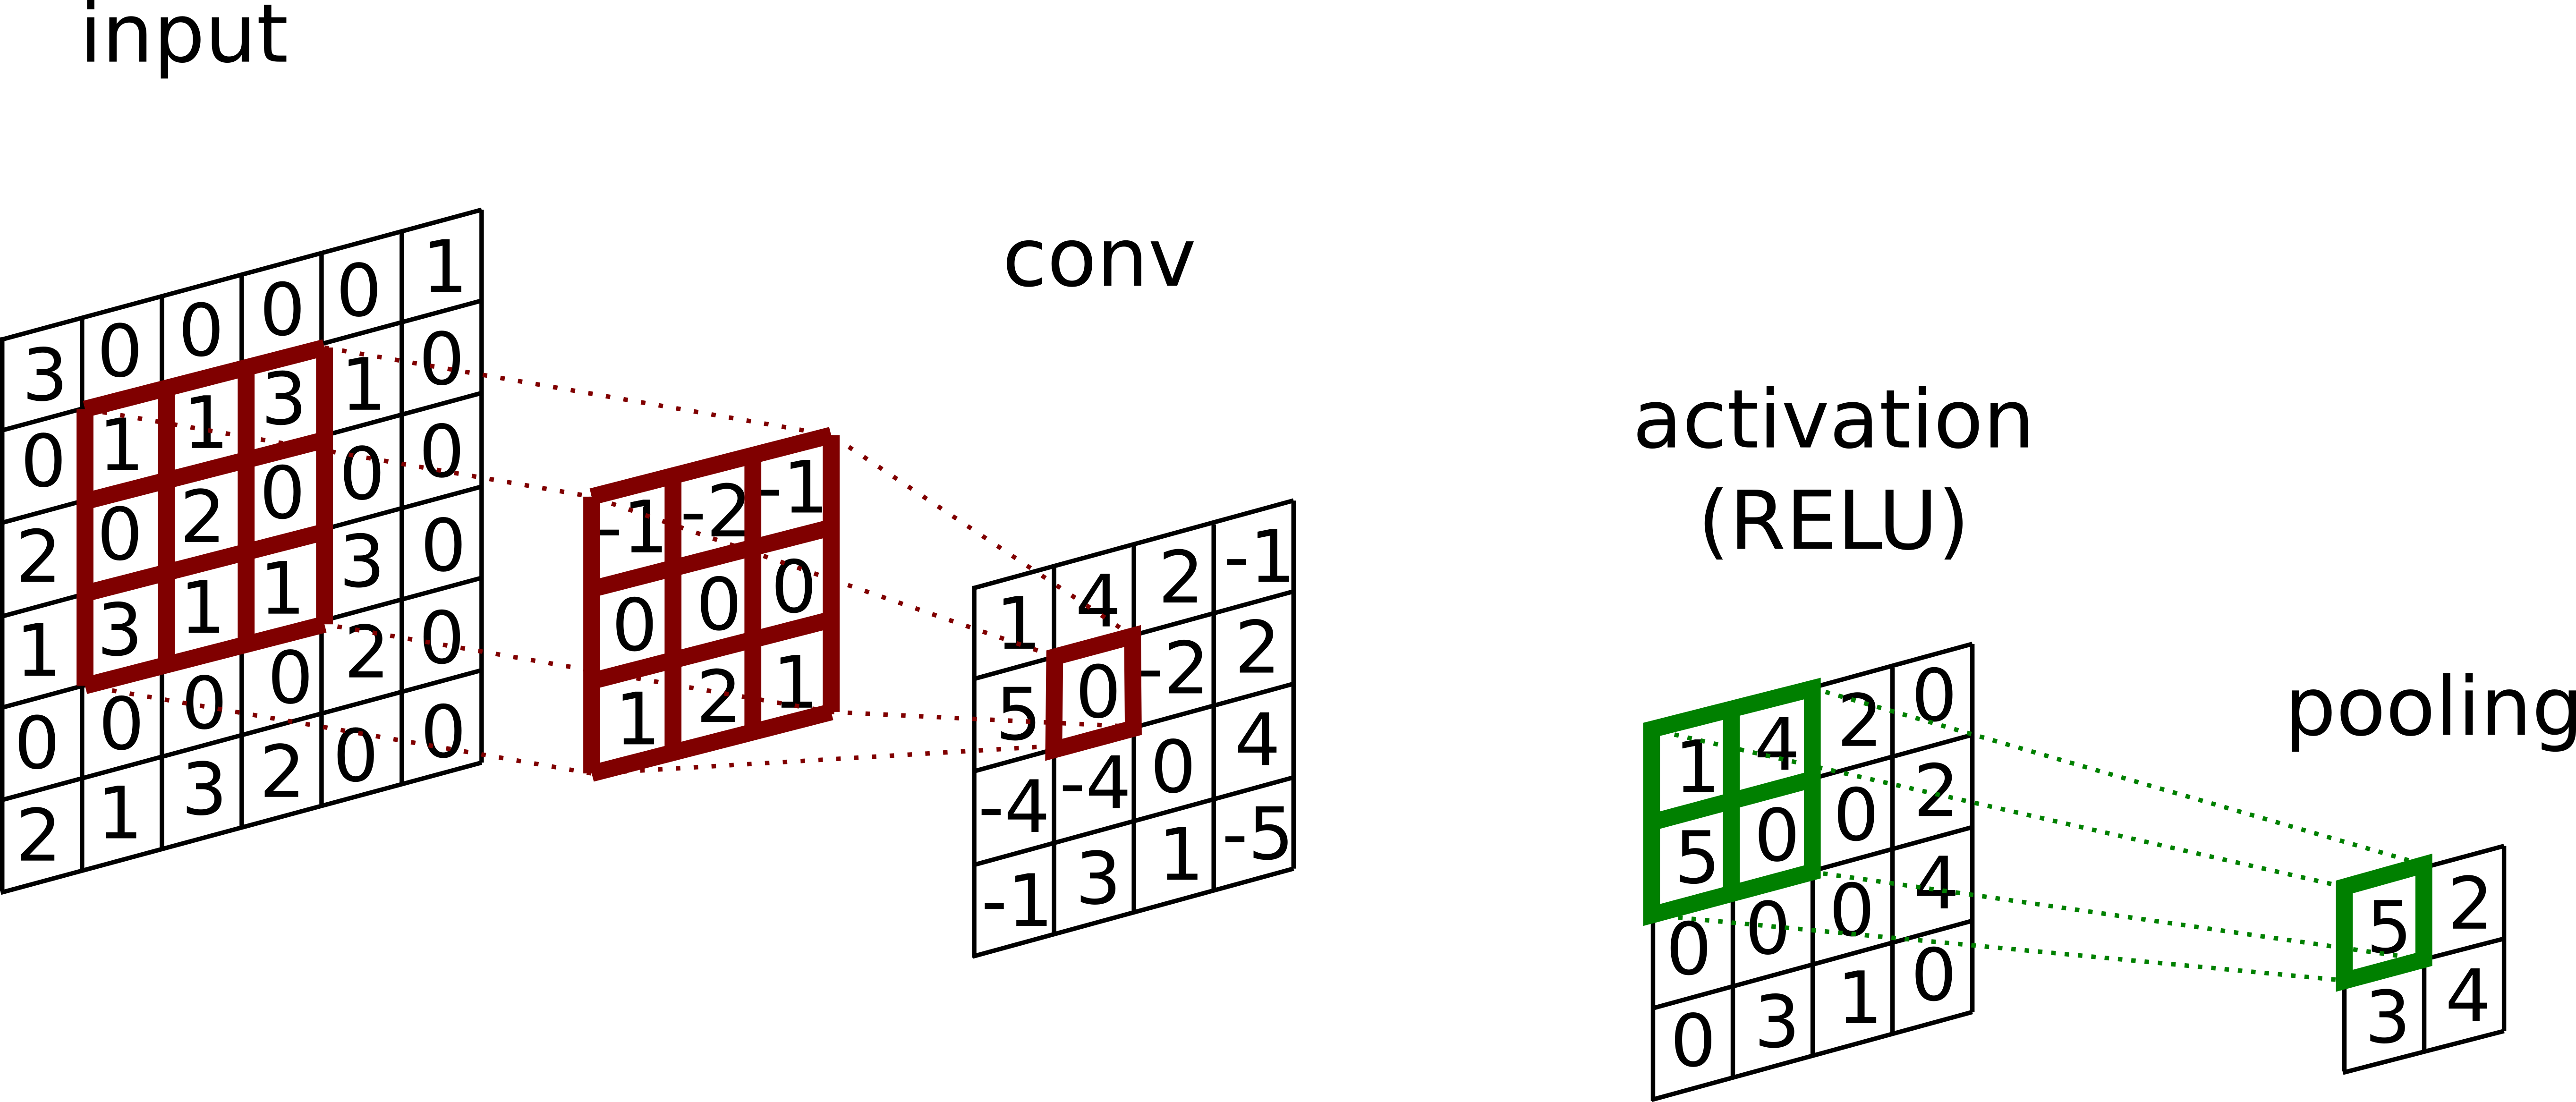
\includegraphics[width=0.55\linewidth, trim={0 0 69cm 0},clip]{imgs/convolution}
		\caption{The input is an image with dimensions 6x6, corresponding to 36 pixels. The kernel is a famous filter called the Sobel filter and is used for edge detection.}
		\label{fig:convolution}
	\end{figure}
	\noindent
	In figure \ref{fig:convolution}, the kernel is simply a 3x3 matrix: 
	\[\medmath{\text{Kernel} = \begin{bmatrix}
			-1 & -2 & -1 & \\ 0 & 0 & 0 &  \\
			1 & 2 & 1
	\end{bmatrix}}  \] 
	One convolution corresponds to multiplying the matrix with every possible space in the 6x6 input image. The stride in this example is one, which refers to how the kernel is moved across the image. If no padding is applied to the input image the dimension of the output image after the convolution will be smaller. In this example the image will shrink from 6x6 to 4x4. To put it simply, the kernel is slid across the width and height of the input and the dot products between the input and kernel are computed at every spatial position \cite{cnn_paper}.
	\\\\
	The kernels in a convolutional neural network are learnable parameters. The dimension of the kernels are smaller than the input, which in turn will reduce the dimension of the input image. All padding are set to zero, which can also be seen in the source code %TODO ref soruce. Har oskar skrevet dette???? tror der er soruce?  
	In this project the three main type of layers in the network model are:

	\begin{itemize}
	\item Convolutional Layers 
	\item ReLU to ensure non-linearity 
	\item Classification in terms of Fully Connected Layers
	\end{itemize}
	\noindent
	The classifier in this project was trained on 80\% of the available data and was tested on the last 20\%. As for hyperparameters consult following table.
	
	\begin{table}[H]\label{hyperparams}
		\centering
		\begin{tabular}{l l l l l l l l l}
			\toprule
			& \textbf{Hyperparameter}           &&&&& & \textbf{Value}    & \\ \midrule
			& Train-test split         &&&&& & $0.8/0.2$& \\
			& Dropout $[p]$            &&&&& & $0.15$    & \\ 
			& Learning rate $[\alpha]$ &&&&& & $0.0002$  & \\ 
			& Epochs                   &&&&& & $230$    & \\  \bottomrule
		\end{tabular}
	\end{table}
	
	 \noindent
	 The optimization algorithm used in the classifier was Adaptive Moment Estimation (Adam). This optimizer utilized adaptive learning rate and step size based on the momentum. The activation function used was ReLU, which is defined as $ y = \text{max}(0,x) $. ReLU ensures non-linearity in the model, making the parameters more expressible and making the model more generalizable and robust. Sigmoid was used on the last layer to ensure that the output value was a vector between zero and one. Cross-entropy loss was used as the cost function and punished the model if the prediction was far from the label \cite {dl}. The loss was calculated using:
	 
	\begin{equation*}\label{key}
		L\left(\boldsymbol{y}_{i}, \hat{\boldsymbol{y}}_{i}\right) = -(\mathbf y \log (\mathbf {\hat y})+(1-\mathbf  y) \log (1-\mathbf {\hat y}))
	\end{equation*}
	\noindent
	The following table will outline the architecture of the model. From the table, each layer with its respective size and trainable parameters will be shown.
	
	
	% ----------------------------------------------------------------
%	Layer (type)               Output Shape         Param #
%	================================================================
%	Conv3d-1    [-1, 32, 254, 143, 119]             896
%	ReLU-2    [-1, 32, 254, 143, 119]               0
%	Conv3d-3      [-1, 64, 126, 71, 59]          55,360
%	ReLU-4      [-1, 64, 126, 71, 59]               0
%	Conv3d-5     [-1, 128, 124, 69, 57]         221,312
%	ReLU-6     [-1, 128, 124, 69, 57]               0
%	Conv3d-7      [-1, 256, 61, 34, 28]         884,992
%	ReLU-8      [-1, 256, 61, 34, 28]               0
%	Conv3d-9      [-1, 512, 57, 30, 24]      16,384,512
%	ReLU-10      [-1, 512, 57, 30, 24]               0
%	Conv3d-11     [-1, 1024, 28, 14, 11]      14,156,800
%	ReLU-12     [-1, 1024, 28, 14, 11]               0
%	Linear-13                  [-1, 128]     565,182,592
%	ReLU-14                  [-1, 128]               0
%	LayerNorm-15                  [-1, 128]             256
%	Dropout-16                  [-1, 128]               0
%	Linear-17                    [-1, 2]             258
%	================================================================
%	Total params: 596,886,978
%	Trainable params: 596,886,978
%	Non-trainable params: 0
%	----------------------------------------------------------------
%	Input size (MB): 17.13
%	Forward/backward pass size (MB): 4193.32
%	Params size (MB): 2276.94
%	Estimated Total Size (MB): 6487.40
% 32x3x3x3 Conv3d, stride 1, pad 0                & 64x257x257     &             & 6,976         \\

	\begin{table}[H]
		\hspace*{-2cm}
		\begin{tabular}{llll}\toprule
			Layer                                       & Activation Size& Value       & \# Parameters \\ \midrule
			Input                                       & 3x256x256      &             & 0             \\
			32x3x3x3 Conv3d, stride 1, pad 0                 & 32x254x143x119       &               & 896         \\
			ReLU                                             & 32x254x143x119       & inplace=False & 0           \\
			64x3x3x3 Conv3d, stride 2, pad 0                 & 64x126x71x59         &               & 55,360        \\
			ReLU                                             & 64x126x71x59         & inplace=False & 0           \\
			128x3x3x3 Conv3d, stride 1, pad 0                & 128x124x69x57        &               & 221,312        \\
			ReLU                                             & 128x124x69x57        & inplace=False & 0           \\
			256x3x3x3 Conv3d, stride 2, pad 0                & 256x61x34x28         &               & 884,992        \\
			ReLU                                             & 256x61x34x28         & inplace=False & 0           \\			512x5x5x5 Conv3d, stride 1, pad 0                & 512x57x30x24         &               & 16,384,512        \\
			ReLU                                             & 512x57x30x24         & inplace=False & 0           \\			
			1024x3x3x3 Conv3d, stride 2, pad 0               & 1024x28x14x11        &               & 14,156,800      \\			ReLU                                             & 1024x28x14x11        & inplace=False & 0           \\			
			Linear                                           & 128                  &               & 565,182,592   \\				
			ReLU                                             & 128                  & inplace=False & 0           \\
			LayerNorm                                        & 128                  &               & 256 \\			Dropout                                          & 128                  & $ p = 0.15 $              & 0 \\
			Linear                                           & 2                    &               & 258   \\							
											
			&                &             &               \\
			\textbf{Total Parameters}                   &                &             & 596,886,978    \\
			\textbf{Trainable Parameters}               &                &             & 596,886,978    \\ \bottomrule
		\end{tabular}
		\caption{The convolutions, stride and padding of each layer in the classification model. The values used in the activation functions and instance normalization (LayerNorm) as well as when they were used in the network have also been shown. Other table details are given in the table \ref{tab:gan_generator} and \ref{tab:discriminator_layers} captions.}
		\label{cnn_arcitecture}
\end{table}	

	\subsubsection{Memory Handling}
	Due to the pure size of the 3D images, which is 256x256x256 for each 3D image, it required enormous amounts of memory on the GPU to run the network outlined in table \ref{cnn_arcitecture}. For this project, 32 GB GPUs were available, which made it feasible to run and train the model with a batch size of 1 and images cropped to size 256x145x121. The reason why cropping was used was due to the amount of black pixels around the brain itself. Other implementations to extend the amount of available memory on the GPU have been implemented in the source code, such as: \texttt{torch.cuda.empty\_cache()}, which empties the cache of the cuda and in turn enables a bit more of memory.



\subsection{Dimensionality Reduction: t-SNE \& PCA}
%TODO Describe method to look at features for 2nd last linear layer

The amount of input features or shape of an input for a model is often referred as the dimensionality of the dataset or variable. The end goal of dimensionality reduction is to reduce the number of features (dimensions) in a given dataset, while keeping as much of the variation in the dataset as possible. This is very useful to visualize high dimensional features in a human interpretable space such as 2D or 3D. Two different dimensionality algorithms have been utilized in this project to investigate if a CNN trained on generated images and original images inherit a bias towards either of the image types. The two algorithms are Principal Component Analysis (PCA) and t-Distributed Stochastic Neighbor Embedding (T-SNE).
\\\\
\textbf{Principle Component Analysis} is a widely used algorithm within the field of machine learning for dimensionality reduction. With large datasets containing many features PCA offers a method that can minimize information loss while increasing the interpretability. This is done by calculating the principle components which is a new set of de-correlated variables that maximizes the variance. A way to calculate the principle component is by using Singular Value Decomposition (SVD), to find the eigenvalues and eigenvectors. Then, the original data can be projected into a space with fewer dimensions. Furthermore, PCA can be used to see how much variance is explained by each of the principle components in a dataset. Thus, PCA is useful for both visualizing and intepreting high dimensional features, but also as a way to reduce the dimension of high dimensional datasets without losing more information than strictly necessary. In this project, PCA was used to project the features of the penultimate linear layer in the CNN to understand and see if the model interpreted 1.5T ground and 1.5T generated images differently \cite{pca1} \cite{pca2}. 
\\\\
\textbf{t-Distributed Stochastic Neighbor Embedding} is another type of dimensionality reduction algorithm, which, much like PCA, can be used to visualize and understand high dimensionality data. The main difference from PCA is that t-SNE  creates a space where points that are close are similar in the original space. Thus, t-SNE will attempt to cluster data with local similarities, but de-prioritize keeping large pair-wise distances between samples (where PCA will prioritize separating dissimilar data). 
From a high-level overview, t-SNE will compare the similarity of two points in both the high-dimensional and low-dimensional space. Then, it will iteratively optimize these measures by using Kullback-Liebler (KL) divergence as a cost function.

A more detailed description of how t-SNE was calculated is outlined below:

\begin{equation}\label{it1}
		p_{i,j} = \frac{\exp(\frac{-\norm{\mathbf x_i - \mathbf x_j}^2}{2 \sigma^2})}{\sum_{k} \sum_{l \neq k} \exp (\frac{-\norm{\mathbf x_k - \mathbf x_l}^2}{2 \sigma^2})}
\end{equation}
Each sample was made the center of a gaussion distribution. Then the distance to all other points within this distribution was measured, using the euclidean distance. The enumerator of equation \eqref{it1} calculated the density of the given point whereas the denominator ensured re-normalization. The variable $ p_{i,j} $ is a probability measure of distance between two samples in a high dimensional space. The probability of a point, $ j $ within the distribution given the point $ i $, is in practice calculated with the following expression.

\begin{equation*}\label{key}
	p_{i \vert j} = \frac{\exp(\frac{-\norm{\mathbf x_i - \mathbf x_j}^2}{2 \sigma_i^2})}{\sum_{j^\prime \neq i} \exp (\frac{-\norm{\mathbf x_i - \mathbf x_{j^\prime}}^2}{2 \sigma_i^2})}
\end{equation*}
\noindent
Of most importance here are $ p_{i \vert i} = 1$  and $ \sum_{j} p_{j \vert i = 1}$. As the author of "Visualizing Data using t-SNE", Laurens van der Maaten,  wrote in her original paper: The similarity of datapoint $ x_j $ to datapoint $ x_i $ is the conditional probability, $ p_{j \vert i} $  that $ x_i $ would pick $ x_j $ as its neighbor if neighbors were picked in proportion to their probability density under a Gaussian centered at $  x_i $ \cite{tsne}.

\begin{equation}\label{symmetry}
	p_{ij} = \frac{	p_{i \vert j} + p_{j \vert i}}{2N}
\end{equation}
\noindent
By using equation \eqref{symmetry}, the conditional probabilities were averaged. This was important because the distance from point x to y might not be equal to the distance from point y to x. 

After the above similarities were calculated, each sample in the data was represented in a low dimensional space. The whole goal from here was to learn a dimensional mapping from the similarities in the high dimensional space to the low dimensional space.

\begin{equation}\label{tdistro}
	q_{i,j} = \frac{(1 + \norm{\mathbf y_i - \mathbf y_j}^2)^{-1}}{\sum_k \sum_{l \neq k}(1 + \norm{\mathbf y_i - \mathbf y_j}^2)^{-1}}
\end{equation}
From equation \eqref{tdistro}, a student-t distribution with 1 as degree of freedom was used to measure the similarities between the low-dimensional points. 
The location of the samples in the mapping process was optimized using the KL divergence as a cost function. The KL divergence measures the similarity of two distributions, in this case: $ P $ and $ Q $. 
\begin{equation*}\label{key}
	KL(Q \vert \vert P) = \sum_{i \neq j} p_{ij} \log \frac{p_{ij}}{q_{ij}}
\end{equation*} 
The minimization process was done using \href{https://scikit-learn.org/stable/modules/generated/sklearn.manifold.TSNE.html}{sklearn} which utilizes gradient decent. The output is a mapping that can visualize the similarities from high dimensional inputs. For this project the input will be a massive linear layer from the CNN. The goal was to map this high dimensional layer into a 2D-space for each sample in the validation data to detect if a difference between the protected classes such as the field strength of the input image or if the input is synthetically generated by a CycleGAN could be seen.


\subsection{Reproducibility}\label{reproducibility}
This section aims to give the reader a precise insight into how the methods of this project were implemented and how it would be possible to reproduce these results in the future. Hopefully, this will simplify the methods. Reproducibility is an important part of writing any project or performing any research. It shows significance of the given result if it is possible for others at a later time to replicate or reproduce the results, since it validates the result of the original study and shows that it was not a fluke. This section was originally adapted from our project work in 2020, so some similarities in layout and wording might occur \cite{fagproject}. By far the most used programming language in this project was Python Version 3.9 and Torch version $ 1.10.0 $ \cite{python, pytorch}.
Furthermore, the versions of the packages used in the project are given in the table below. If running any code from this project, please make sure that your packages either as new or newer than the ones specified below \footnote{Be aware that newer version of packages might have changes that can affect the results of this report. If the goal is to reproduce the results 1:1, please ensure that every package is the exact version as specified in table \ref{tab:packages}.}. All code for the project is accessible at \url{https://github.com/oskarwiese/AlzPred/tree/main/oskar_implemetation}. Note, that the data preprocessing have been described in section \ref{preprocess_scripts} and the code for this can be seen in appendix[\ref{appendix}], consult figure \ref{script1} \& \ref{script2}. 

\begin{table}[H]
	\begin{center}
		\begin{tabular}{l l l l l l l l l l}
			\toprule			
			
			& \textbf{Package \cite{python_packages}}      & & & & & & & \textbf{Version}  & \\ \midrule
			& albumentations \cite{albumentations}         & & & & & & & $1.1.0$           & \\ 
			& ipython \cite{ipython}                       & & & & & & & $7.30.1$          & \\ 
			& matplotlib \cite{matplotlib}                 & & & & & & & $3.5.0$           & \\ 
			& nipy \cite{nipy}                             & & & & & & & $0.5.0$           & \\
			& pandas \cite{pandas}                         & & & & & & & $1.3.5$           & \\
			& pelutils \cite{pelutils}                     & & & & & & & $0.6.9$           & \\
			& pip-chill \cite{pip-chill}                   & & & & & & & $1.0.1$           & \\
			& torchio \cite{torchio}                       & & & & & & & $0.18.71$         & \\
			& torchsummary \cite{torchsummary}             & & & & & & & $1.5.1$           & \\
			& torch \cite{pytorch}                         & & & & & & & $1.10.0+cu113$    & \\
			& torchvision \cite{torchvision}               & & & & & & & $0.11.1+cu113$    & \\
			\bottomrule
		\end{tabular}
		\caption{The packages used for all the scrips in this project as well as their versions. Note that \texttt{pip-chill} was only used to generate this table and \texttt{ipython} is not strictly necessary, but nice for debugging \& testing simple pytorch operations.}
		\label{tab:packages}
	\end{center}
\end{table}
\noindent Since randomness plays a large roll in implementing deep learning architectures, random seeds have been set in order to ensure equivalent results for every run of every code block. The seed number was set to 42 and was used for the python seed \texttt{random.seed}, the numpy seed \texttt{np.random.seed} and the pytorch seeds \newline \texttt{torch.manual\_seed}, \texttt{torch.cuda.manual\_seed} and 
\texttt{torch.cuda.manual\_seed\_all}. These seeds were set before any processes run in any of the scrips used.
\\\\
In order to make the results as reproducible as possible, the data as well as the way the data was obtained also plays a big role. The data originally comes from the ADNI studies\footnote{A more detailed outline of the data is given in section \ref{dataDescription}}, but the specific preprocessed data for this project are located in the following folders on the HPC / dtu server: \texttt{/dtu-compute/ADNIbias/freesurfer\_ADNI1} and \texttt{/dtu-compute/ADNIbias/freesurfer\_ADNI2}. Furthermore, 3T images of validation subjects are located at: \texttt{/dtu-compute/ADNIbias/freesurfer}  \footnote{All the folders can be found on the DTU HPC server with the given absolute paths.}. \\

\noindent
There are two main code structures which will be explained in more detail in the following. These are the scripts that were used to construct and train the CycleGAN and CNN classifier models used in this project. 
\\\\
\noindent Below, a thorough walkthrough of the most essential parts of the code for the CycleGAN will be made. The code is split between six different files, the names and short descriptions of which can be seen in table \ref{fig:files}. 
%TODO tilføj reconstruct.py 
\begin{table}[H]
		\hspace*{-2cm}
		\begin{tabular}{l l l l l l l l l}
			\toprule
			& \textbf{File}          & & & & & & \textbf{Description}  & \\ \midrule
			& train.py               & & & & & & \makecell[tl]{Main script which runs the training loop \\ and saves the final models} & \\
			& discriminator\_model.py& & & & & & Definition of the discriminator architecture & \\
			& generator\_model.py    & & & & & & Definition of the generator architecture & \\
			& utils.py               & & & & & & \makecell[tl]{Utility functions like plotting, save/load \\ checkpoint and seeding} & \\
			& data\_load.py             & & & & & & Preprocessing of the dataset & \\
			& plot.py             & & & & & & Script for plotting loss & \\
			& config.py              & & & & & & Paths and hyperparameter definition & \\ \bottomrule
		\end{tabular}
\caption{CycleGAN code description}
\label{fig:files}
\end{table}

\noindent
The primary file is \texttt{train.py}, which is responsible for putting all of the functionality together. This script starts by defining each of the four models (generators/discriminators) as well as the optimizers and losses. Afterwards, it loads in the dataset and starts the training loop. This loop calls the function \texttt{train\_cykel} where all model interactions and singular losses are immediately calculated. Afterwards, adversarial loss, cycle-consistency loss and identity loss are found and added to get the final loss. This loss is then backpropagated through the model and the next batch is run.
\\\\
The next two files, \texttt{discriminator\_model.py} and \texttt{generator\_model.py} are related in the sense that they both define the general functionality of models used in \texttt{train.py}. In \texttt{discriminator\_model.py}, the \texttt{Block} class defines the architecture of using one convolution and applying instance normalization and leaky-ReLU, which becomes useful often. The class \texttt{Discriminator} is the workhorse of the script. This class initially defines a layer applying a 2D convolution and leaky-ReLU, after which a number of blocks are added. At the end of the architecture, a last convolutional layer is added and sigmoid is applied to output probabilities. In the script \texttt{generator\_model.py}, the \texttt{ConvBlock} class defines a convolution consisting of a 2D convolution, instance normalization and applying ReLU. The \texttt{ResidualBlock} class consists of two \texttt{ConvBlock} calls. Both of these classes help to implement the general architecture in the \texttt{Generator} class. The \texttt{Generator} class has an initializer made up of an initial layer, down-blocks, up-blocks, residual blocks and a last layer. These are called in the forward method, where an initial layer is first added, then the down-blocks, the residual blocks, the up-blocks and at last the final layer. On top of this, tan-h is applied to the model output.
\\\\
The script \texttt{config.py} is very short but extremely important for the general workflow and successful use of the code. It defines the directories of the data and almost all hyperparameters that might need to be changed at any point for any reason when running the code.
\\\\
The script \texttt{utils.py} and \texttt{data\_load.py} are not as important to the general workflow and are much easier to understand. \texttt{utils.py} simply implements functions that save and load a checkpoint (current model and optimizer states) such that training can easily be stopped or the best model can be saved. Functions are also saved to plot the loss curves and add seeds to everything, so randomness does not provide difficulty. \texttt{data\_load.py} does all the data preprocessing.
\\\\
\noindent Below, a thorough walkthrough of the most essential parts of the code for the CNN classifier will be made. The code is split between six different files, the names and short descriptions of which can be seen in table \ref{fig:files}. 

\begin{table}[H]
			\hspace*{-2cm}
		\begin{tabular}{l l l l l l l l l}
			\toprule
			& \textbf{File}          & & & & & & \textbf{Description}  & \\ \midrule
			& train\_classifier.py               & & & & & & \makecell[tl]{Main script which runs the training loop \\ and saves the final models} & \\
			& classifier\_model.py& & & & & & Definition of the classifier architecture & \\
			& utils.py               & & & & & & \makecell[tl]{Utility functions for augmentation, save/load etc.} & \\
			& data\_prep.py             & & & & & & Preprocessing of the dataset & \\
			& feature\_visualization.py              & & & & & & Script for visualizing feature representation. & \\ \bottomrule
		\end{tabular}
	\caption{CycleGAN code description}
	\label{fig:files_CNN_classifier}
\end{table}

\noindent
The primary file is \texttt{train\_classifer.py}, which is responsible for putting all of the functionality together. This script starts by reading the data and turning it into a PyTorch data-loader object. Then, the model is initialized along with the optimizer. Then the training loop starts, which ensures training of the model interactions and singular losses are immediately calculated after prediction on the training set. Afterwards the loss is backpropagated through the entire network. Once this is done, evaluation mode is turned on and the model is tested on the validation set.  Afterwards, loss is calculated. The losses are then appended to a list for visualization of the model performance.
\\\\
The next file, \texttt{classifer\_model.py}, defines the general functionality of the CNN classifier models used in \texttt{train\_classifier.py}. In the script, a class is defined, namely, \texttt{ConvNet}, which includes the architecture of the classifier. Six 3D convolutional layers and two linear layers. Furthermore, it includes the forward function, which is used to forward the input through the network. 
\\\\
The script \texttt{utils.py} and \texttt{data\_prep.py} are not as important to the general workflow and are much easier to understand. \texttt{utils.py} simply implements functions that save the model (current model and optimizer states) such that training can easily be stopped or the best model can be saved. Functions are also saved to plot the loss curves and augmentation. \texttt{data\_prep.py} does all the data preparation.
\\\\
Lastly, \texttt{feature\_visualization.py} is used to construct 2D-plots of the high dimensional features from the 2nd last linear layer in the CNN model. It creates both PCA and t-SNE plots.



\section{Results}\label{results}
%TODO: tror ikke alle subsections er nævnt her. Så vi skal nok endten nævne alle eller ingen 
This section will focus on showing relevant outputs of the final trained models. Results from previous, less successful models can be found in section \ref{troubleshooting}, which also highlights some of largest issues during the image generation and how they were solved. The general goal of this section will be to first go through examples of generated images and compare and contrast them to real images, and secondly to show loss-curves for each model. Sections \ref{xy_generated}, \ref{xz_generated} and \ref{yz_generated} provide examples of generated images from the models trained on the $XY$, $XZ$ and $YZ$ respectively. In a slightly different manner, section \ref{training_progress} shows how training comes along after a number of steps to show what the generators learn and when. Afterwards, section \ref{all_generated} will show results on every plane when a model has been trained on data from all of $XY$, $XZ$ and $YZ$. Afterwards, the next four sections will focus on the various losses. The sections \ref{disc_loss}, \ref{gen_loss}, \ref{cycle_loss} and \ref{iden_loss} will show respectively the discriminator losses, generator losses, cycle losses and identity losses from each of the four aforementioned models.

\subsection{Discriminator Losses}\label{disc_loss}
\begin{figure}[H]
	\centering
	\begin{subfigure}[b]{0.8\textwidth}
		\centering
		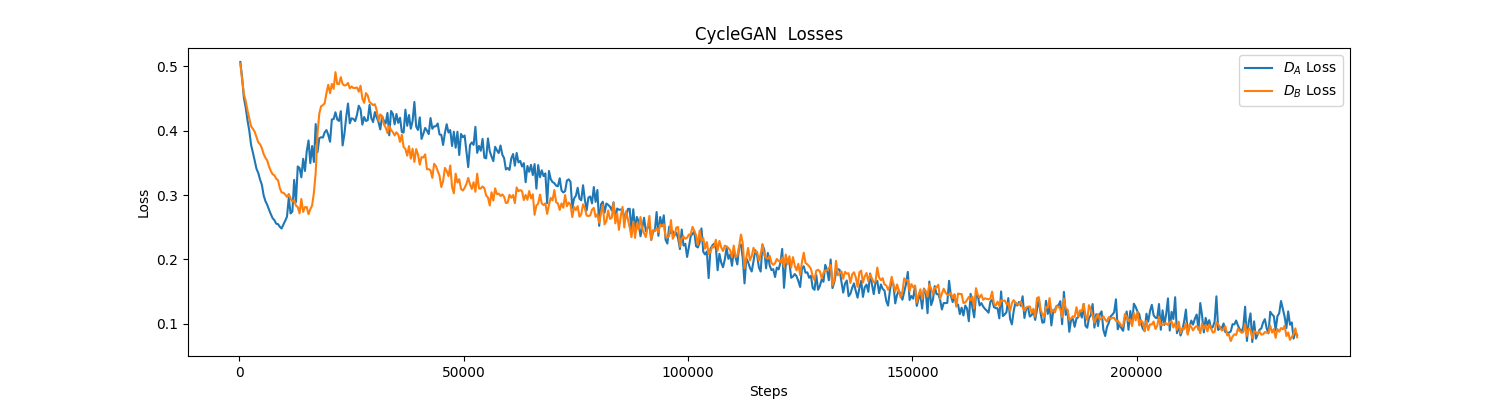
\includegraphics[width=\linewidth]{imgs/discriminator_losses/XY_model_discriminator_losses}
		\hfill
		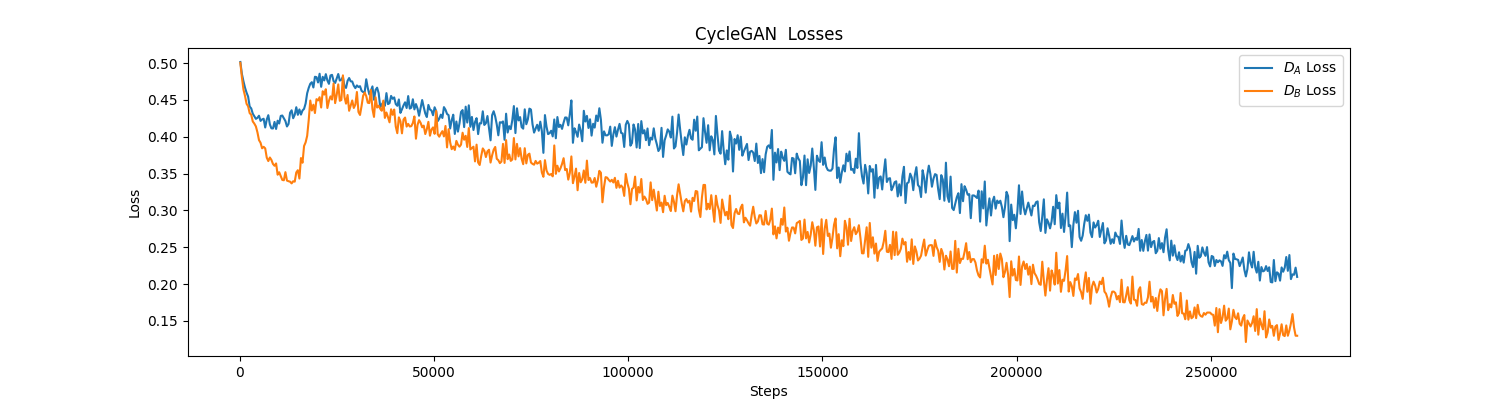
\includegraphics[width=\linewidth]{imgs/discriminator_losses/XZ_model_discriminator_losses}
		\hfill
		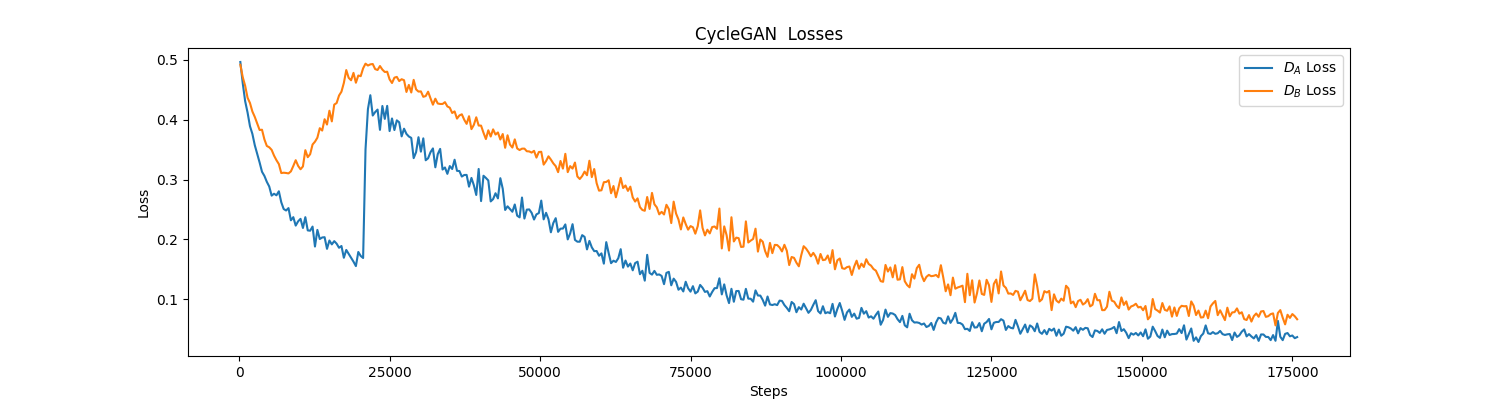
\includegraphics[width=\linewidth]{imgs/discriminator_losses/YZ_model_discriminator_losses}
		\hfill
		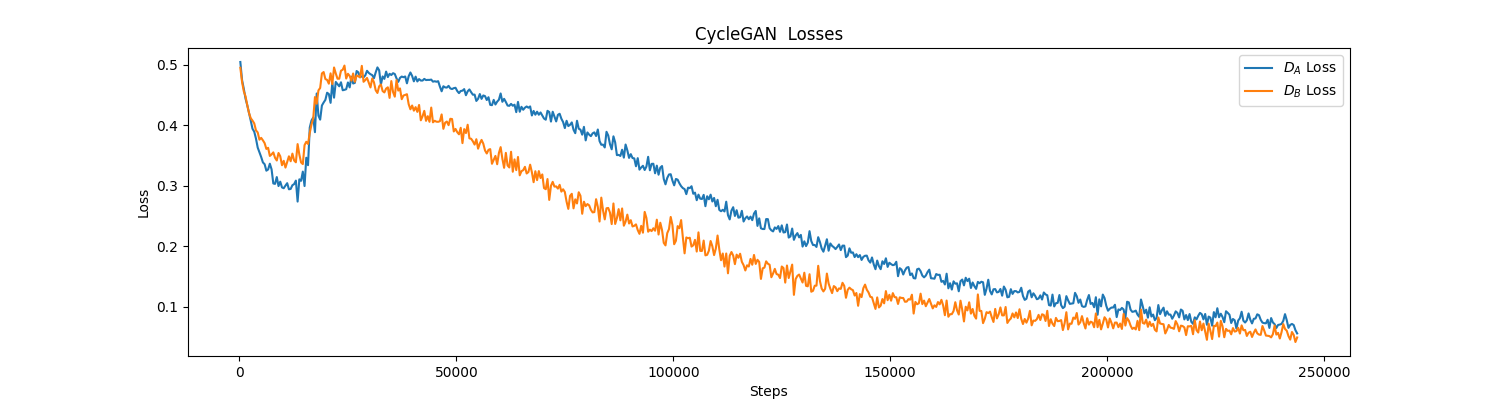
\includegraphics[width=\linewidth]{imgs/discriminator_losses/ALL_model_discriminator_losses}
	\end{subfigure}
	\caption{Discriminator losses for respectively the XY, XZ, YZ and ALL model. $D_A$ tries to predict validity of real and fake 1.5T images and $D_B$ predicts 3T images. The models have been trained with different parameters and for different periods of time, so this loss is not necessarily useful for gauging the model performance. Nevertheless, the figures can be used to determine convergence and signs of learning.}
	\label{fig:discriminator_losses}
\end{figure}

\subsection{Generator Losses}\label{gen_loss}
\begin{figure}[H]
	\centering
	\begin{subfigure}[b]{0.8\textwidth}
		\centering
		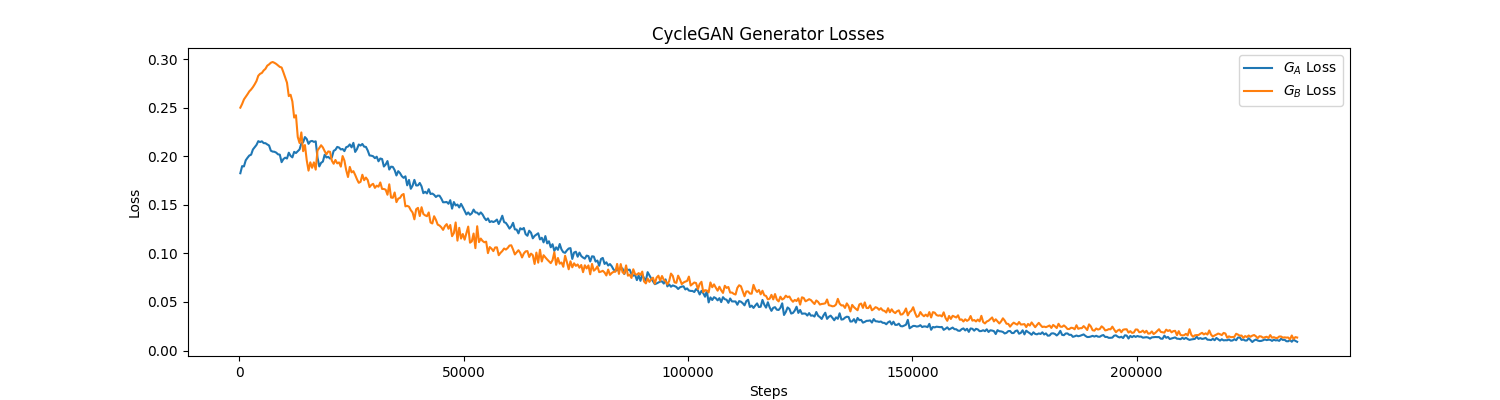
\includegraphics[width=\linewidth]{imgs/generator_losses/XY_model_generator_losses}
		\hfill
		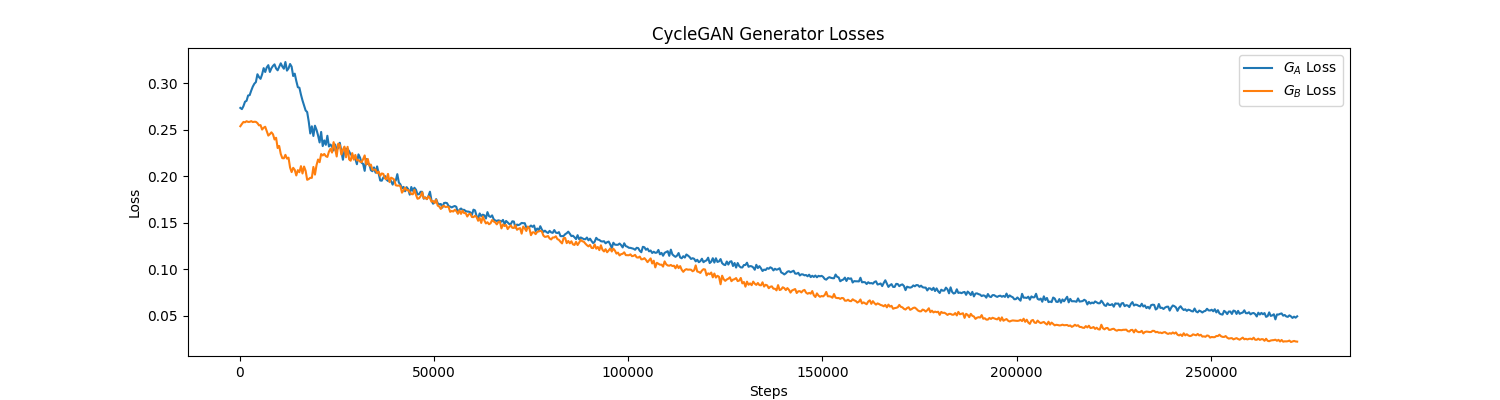
\includegraphics[width=\linewidth]{imgs/generator_losses/XZ_model_generator_losses}
		\hfill
		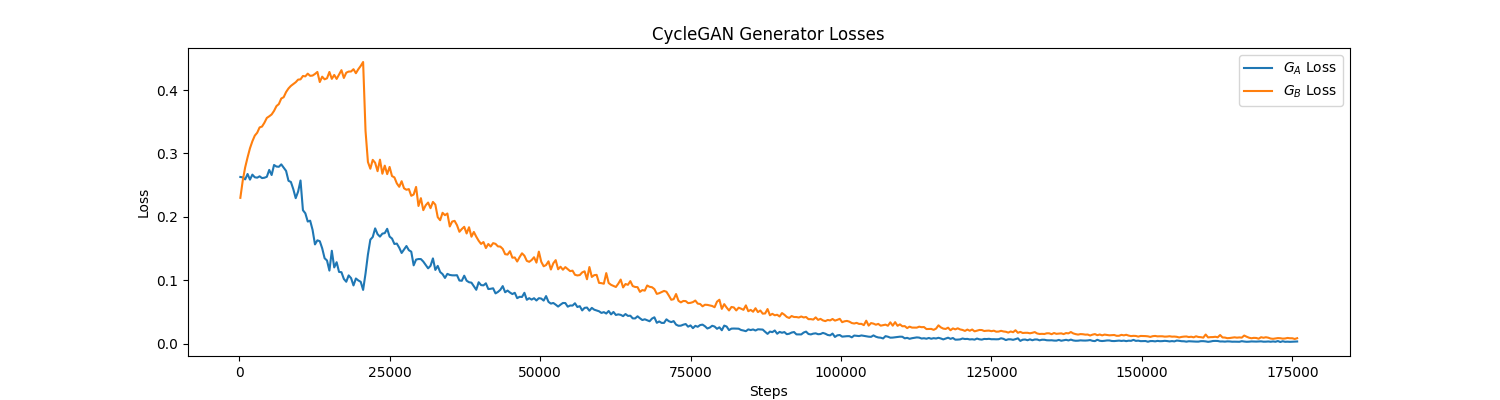
\includegraphics[width=\linewidth]{imgs/generator_losses/YZ_model_generator_losses}
		\hfill
		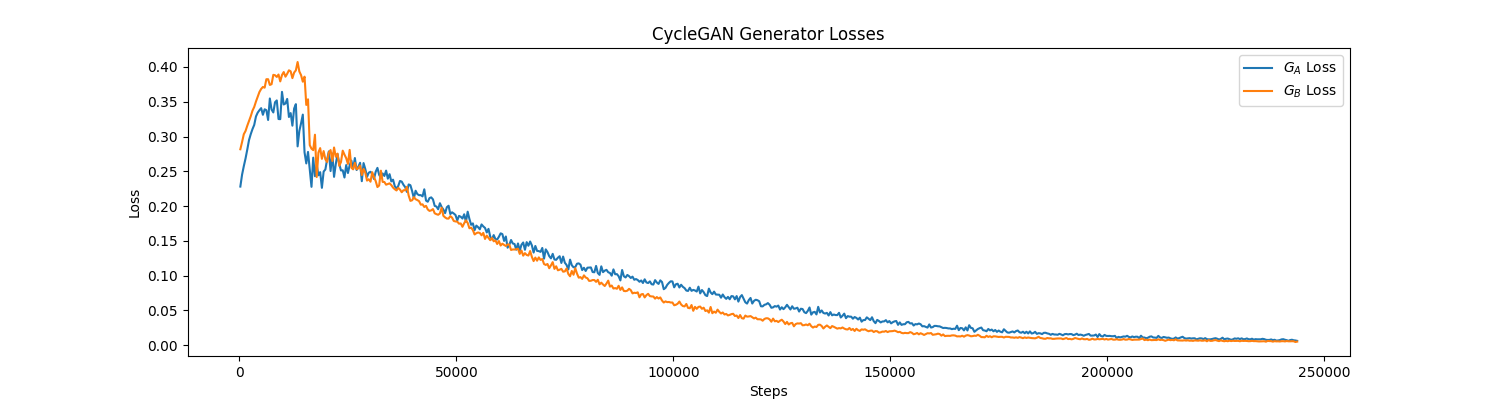
\includegraphics[width=\linewidth]{imgs/generator_losses/ALL_model_generator_losses}
	\end{subfigure}
	\caption{Generator losses for the XY, XZ, YZ and ALL models. $G_A$ converts images from 3T to 1.5T and $G_B$ converts from 1.5T to 3T. Other minutia about the plot is written about in the caption of figure \ref{fig:discriminator_losses}.}
	\label{fig:generator_losses}
\end{figure}

\subsection{Cycle-Consistency Losses}\label{cycle_loss}
\begin{figure}[H]
	\centering
	\begin{subfigure}[b]{0.8\textwidth}
		\centering
		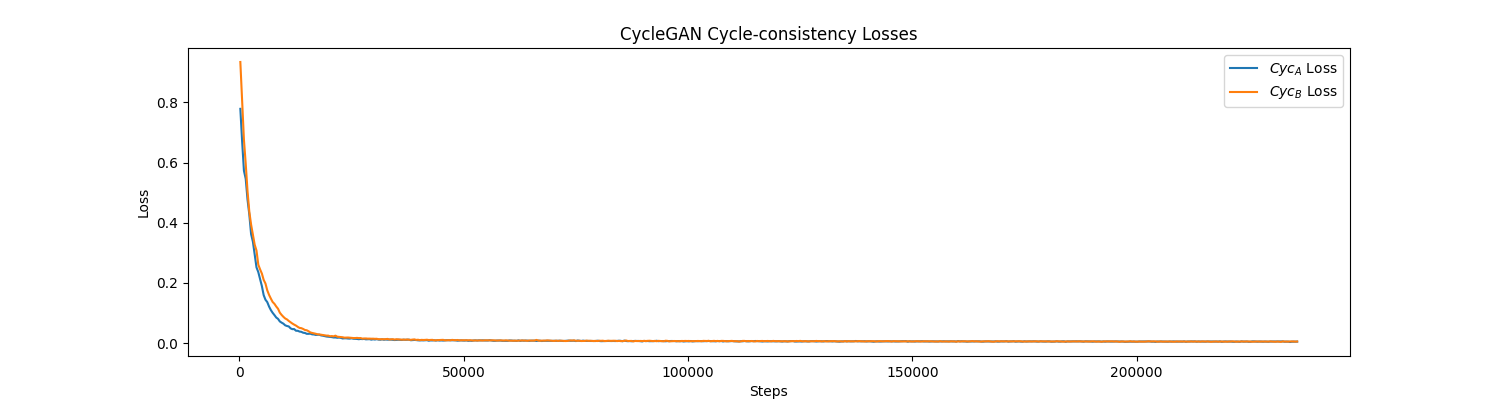
\includegraphics[width=\linewidth]{imgs/cycle_losses/XY_model_cycle_losses}
		\hfill
		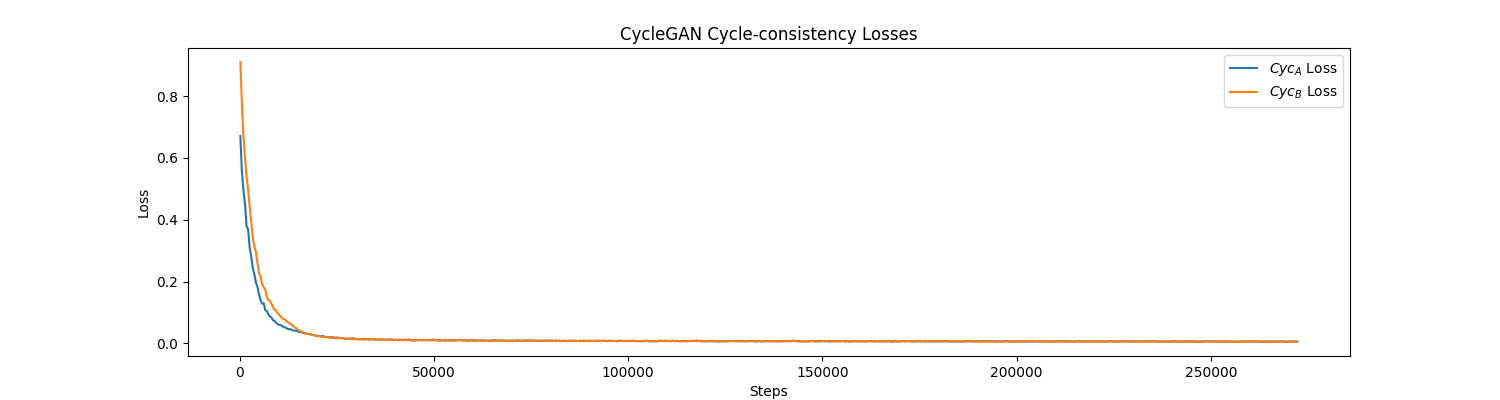
\includegraphics[width=\linewidth]{imgs/cycle_losses/XZ_model_cycle_losses}
		\hfill
		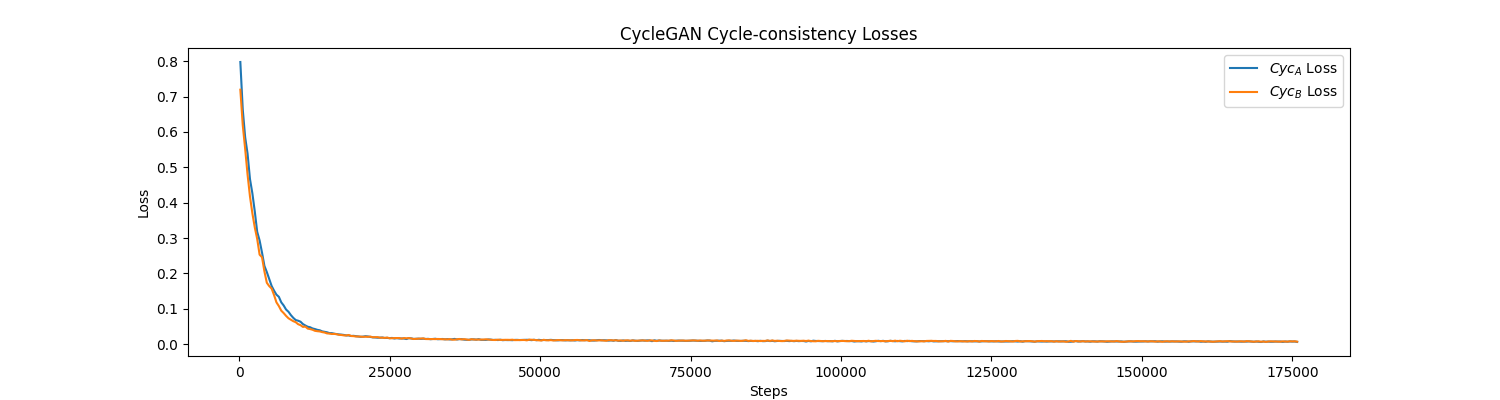
\includegraphics[width=\linewidth]{imgs/cycle_losses/YZ_model_cycle_losses}
		\hfill
		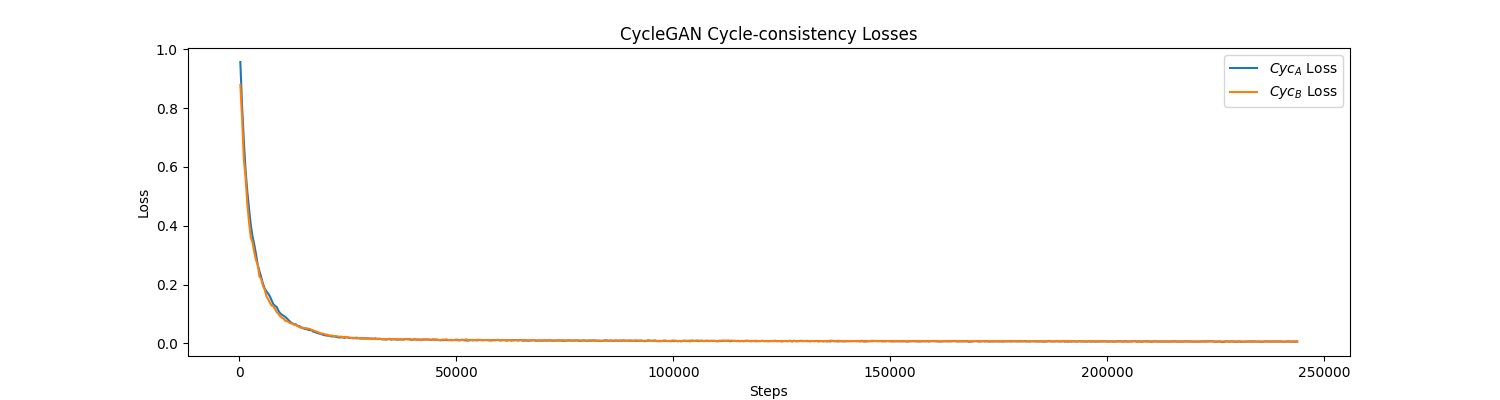
\includegraphics[width=\linewidth]{imgs/cycle_losses/ALL_model_cycle_losses}
	\end{subfigure}
	\caption{Cycle-consistency losses for the XY, XZ, YZ and ALL models. Details are described in the captions of figures \ref{fig:discriminator_losses} and \ref{fig:generator_losses}.}
	\label{fig:cycle_losses}
\end{figure}

\subsection{Identity Losses}\label{iden_loss}
\begin{figure}[H]
	\centering
	\begin{subfigure}[b]{0.8\textwidth}
		\centering
		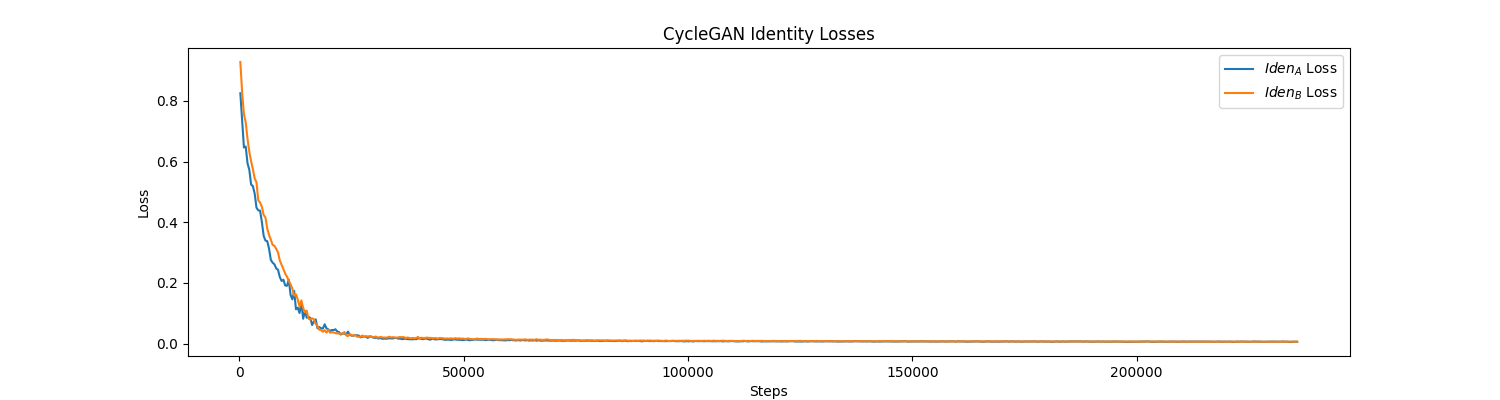
\includegraphics[width=\linewidth]{imgs/identity_losses/XY_model_identity_losses}
		\hfill
		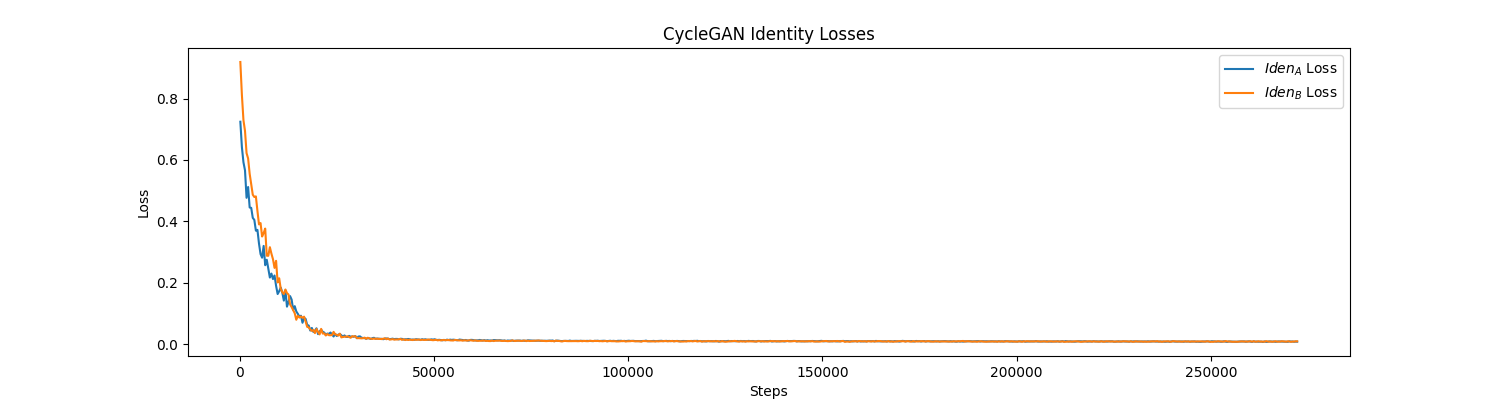
\includegraphics[width=\linewidth]{imgs/identity_losses/XZ_model_identity_losses}
		\hfill
		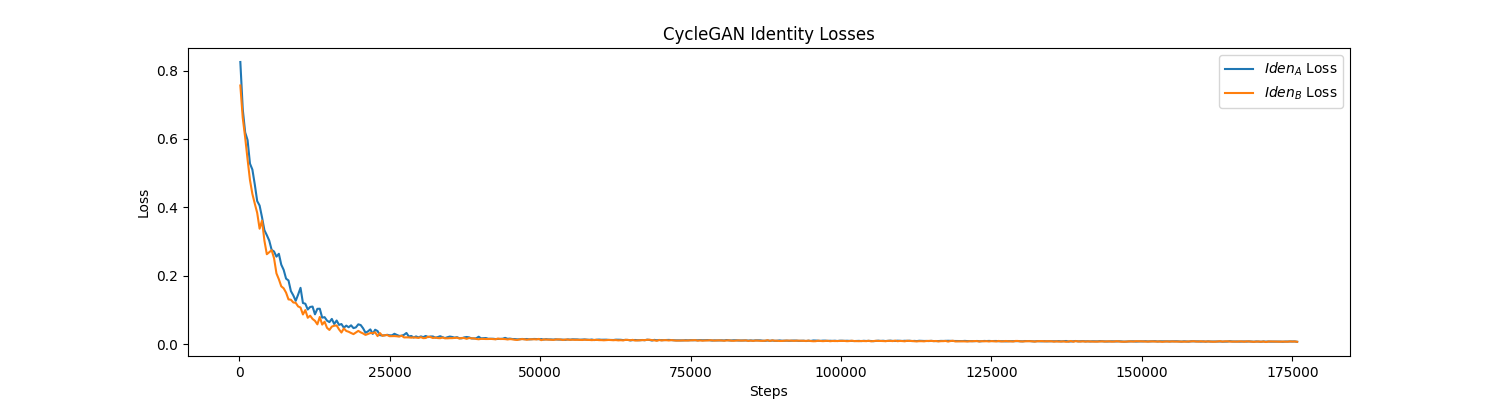
\includegraphics[width=\linewidth]{imgs/identity_losses/YZ_model_identity_losses}
		\hfill
		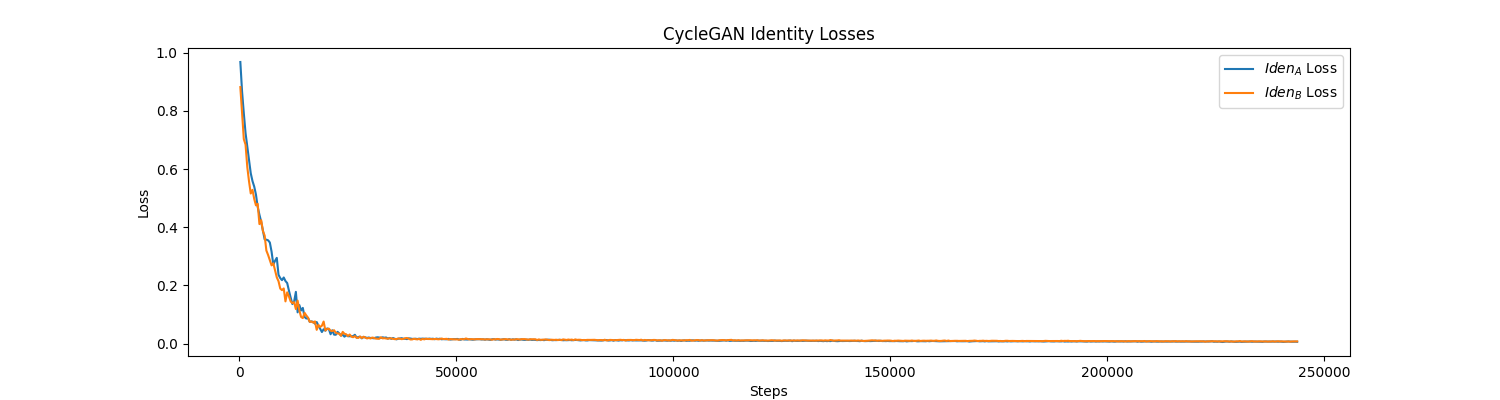
\includegraphics[width=\linewidth]{imgs/identity_losses/ALL_model_identity_losses}
	\end{subfigure}
	\caption{Identity losses for the XY, XZ, YZ and ALL models. Details are described in the captions of figures \ref{fig:discriminator_losses} and \ref{fig:generator_losses}.}
	\label{fig:cycle_losses}
\end{figure}


\subsection{Training Progress}\label{training_progress}
\begin{figure}[H]
	\centering
	\begin{subfigure}[b]{0.7\textwidth}
		\centering
		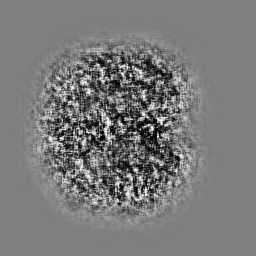
\includegraphics[width=0.22\linewidth]{imgs/training_progress/XY_model_3T_epoch_0_idx_0}
		\hskip\skipper
		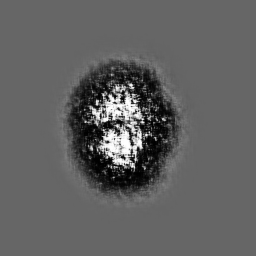
\includegraphics[width=0.22\linewidth]{imgs/training_progress/XY_model_3T_epoch_0_idx_1000}
		\hskip\skipper
		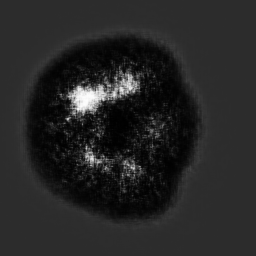
\includegraphics[width=0.22\linewidth]{imgs/training_progress/XY_model_3T_epoch_0_idx_5000}
		\hskip\skipper
		\includegraphics[width=0.22\linewidth]{imgs/training_progress/XY_model_3T_epoch_0_idx_9000}
	\end{subfigure}
	\vskip\ripper
	\begin{subfigure}[b]{0.7\textwidth}
		\centering
		\includegraphics[width=0.22\linewidth]{imgs/training_progress/XY_model_3T_epoch_0_idx_11000}
		\hskip\skipper
		\includegraphics[width=0.22\linewidth]{imgs/training_progress/XY_model_3T_epoch_0_idx_13000}
		\hskip\skipper
		\includegraphics[width=0.22\linewidth]{imgs/training_progress/XY_model_3T_epoch_0_idx_17000}
		\hskip\skipper
		\includegraphics[width=0.22\linewidth]{imgs/training_progress/XY_model_3T_epoch_0_idx_19000}
	\end{subfigure}
	\vskip\ripper
	\begin{subfigure}[b]{0.7\textwidth}
		\centering
		\includegraphics[width=0.22\linewidth]{imgs/training_progress/XY_model_3T_epoch_0_idx_22000}
		\hskip\skipper
		\includegraphics[width=0.22\linewidth]{imgs/training_progress/XY_model_3T_epoch_0_idx_27000}
		\hskip\skipper
		\includegraphics[width=0.22\linewidth]{imgs/training_progress/XY_model_3T_epoch_1_idx_0}
		\hskip\skipper
		\includegraphics[width=0.22\linewidth]{imgs/training_progress/XY_model_3T_epoch_1_idx_77000}
	\end{subfigure}
	\caption{Examples of different slices from the XY model after 0, 1000, 5000, 9000, 11000, 13000, 17000, 19000, 22000, 27000 and 240000 steps respectively from left-to-right, top-to-bottom. The slices where the most interesting developments happen have been chosen. The bottom-left image is generated from the finished model. Note that the subject used to generate each image is random.}
	\label{fig:training_progress}
\end{figure}



\subsection{XY Quality Comparison}\label{xy_generated}
\begin{figure}[H]
	\centering
	\begin{subfigure}[b]{0.7\textwidth}
		\centering
		\includegraphics[width=0.22\linewidth]{imgs/136_S_0196/136_S_0196_xy_3_GT}
		\hskip\skipperer
		\includegraphics[width=0.22\linewidth]{imgs/136_S_0196/XY_model_136_S_0196_xy_1.5}
		\hskip\bigskipx
		\includegraphics[width=0.22\linewidth]{imgs/136_S_0196/136_S_0196_xy_1.5_GT}
		\hskip\skipperer
		\includegraphics[width=0.22\linewidth]{imgs/136_S_0196/XY_model_136_S_0196_xy_3}
	\end{subfigure}
	\vskip\ripperer
	\begin{subfigure}[b]{0.7\textwidth}
		\centering
		\includegraphics[width=0.22\linewidth]{imgs/136_S_0196/136_S_0196_xz_3_GT}
		\hskip\skipperer
		\includegraphics[width=0.22\linewidth]{imgs/136_S_0196/XY_model_136_S_0196_xz_1.5}
		\hskip\bigskipx
		\includegraphics[width=0.22\linewidth]{imgs/136_S_0196/136_S_0196_xz_1.5_GT}
		\hskip\skipperer
		\includegraphics[width=0.22\linewidth]{imgs/136_S_0196/XY_model_136_S_0196_xz_3}
	\end{subfigure}
	\vskip\ripperer
	\begin{subfigure}[b]{0.7\textwidth}
		\centering
		\includegraphics[width=0.22\linewidth]{imgs/136_S_0196/136_S_0196_yz_3_GT}
		\hskip\skipperer
		\includegraphics[width=0.22\linewidth]{imgs/136_S_0196/XY_model_136_S_0196_yz_1.5}
		\hskip\bigskipx
		\includegraphics[width=0.22\linewidth]{imgs/136_S_0196/136_S_0196_yz_1.5_GT}
		\hskip\skipperer
		\includegraphics[width=0.22\linewidth]{imgs/136_S_0196/XY_model_136_S_0196_yz_3}
	\end{subfigure}
	\vskip\bigskipy
	\begin{subfigure}[b]{0.7\textwidth}
		\centering
		\includegraphics[width=0.22\linewidth]{imgs/082_S_0469/082_S_0469_xy_3_GT}
		\hskip\skipperer
		\includegraphics[width=0.22\linewidth]{imgs/082_S_0469/XY_model_082_S_0469_xy_1.5}
		\hskip\bigskipx
		\includegraphics[width=0.22\linewidth]{imgs/082_S_0469/082_S_0469_xy_1.5_GT}
		\hskip\skipperer
		\includegraphics[width=0.22\linewidth]{imgs/082_S_0469/XY_model_082_S_0469_xy_3}
	\end{subfigure}
	\vskip\ripperer
	\begin{subfigure}[b]{0.7\textwidth}
		\centering
		\includegraphics[width=0.22\linewidth]{imgs/082_S_0469/082_S_0469_xz_3_GT}
		\hskip\skipperer
		\includegraphics[width=0.22\linewidth]{imgs/082_S_0469/XY_model_082_S_0469_xz_1.5}
		\hskip\bigskipx
		\includegraphics[width=0.22\linewidth]{imgs/082_S_0469/082_S_0469_xz_1.5_GT}
		\hskip\skipperer
		\includegraphics[width=0.22\linewidth]{imgs/082_S_0469/XY_model_082_S_0469_xz_3}
	\end{subfigure}
	\vskip\ripperer
	\begin{subfigure}[b]{0.7\textwidth}
		\centering
		\includegraphics[width=0.22\linewidth]{imgs/082_S_0469/082_S_0469_yz_3_GT}
		\hskip\skipperer
		\includegraphics[width=0.22\linewidth]{imgs/082_S_0469/XY_model_082_S_0469_yz_1.5}
		\hskip\bigskipx
		\includegraphics[width=0.22\linewidth]{imgs/082_S_0469/082_S_0469_yz_1.5_GT}
		\hskip\skipperer
		\includegraphics[width=0.22\linewidth]{imgs/082_S_0469/XY_model_082_S_0469_yz_3}
	\end{subfigure}
	\caption{Comparing generated images from the XY model to real ground truth images. The columns, from left to right, contain respectively 1.5T ground truth images, 1.5T  generated, 3T ground truth and 3T generated images. As such, the left part of the figure contains only 1.5T images and the right side only contains 3T images. \textbf{Top:} images for subject \texttt{136\_S\_0196}. \textbf{Bottom:} images for subject \texttt{082\_S\_0469}.}
	\label{fig:xy_quality_comparison}
\end{figure}

\subsection{XZ Quality Comparison}\label{xz_generated}
\begin{figure}[H]
	\centering
	\begin{subfigure}[b]{0.7\textwidth}
		\centering
		\includegraphics[width=0.22\linewidth]{imgs/136_S_0196/136_S_0196_xy_3_GT}
		\hskip\skipperer
		\includegraphics[width=0.22\linewidth]{imgs/136_S_0196/XZ_model_136_S_0196_xy_1.5}
		\hskip\bigskipx
		\includegraphics[width=0.22\linewidth]{imgs/136_S_0196/136_S_0196_xy_1.5_GT}
		\hskip\skipperer
		\includegraphics[width=0.22\linewidth]{imgs/136_S_0196/XZ_model_136_S_0196_xy_3}
	\end{subfigure}
	\vskip\ripperer
	\begin{subfigure}[b]{0.7\textwidth}
		\centering
		\includegraphics[width=0.22\linewidth]{imgs/136_S_0196/136_S_0196_xz_3_GT}
		\hskip\skipperer
		\includegraphics[width=0.22\linewidth]{imgs/136_S_0196/XZ_model_136_S_0196_xz_1.5}
		\hskip\bigskipx
		\includegraphics[width=0.22\linewidth]{imgs/136_S_0196/136_S_0196_xz_1.5_GT}
		\hskip\skipperer
		\includegraphics[width=0.22\linewidth]{imgs/136_S_0196/XZ_model_136_S_0196_xz_3}
	\end{subfigure}
	\vskip\ripperer
	\begin{subfigure}[b]{0.7\textwidth}
		\centering
		\includegraphics[width=0.22\linewidth]{imgs/136_S_0196/136_S_0196_yz_3_GT}
		\hskip\skipperer
		\includegraphics[width=0.22\linewidth]{imgs/136_S_0196/XZ_model_136_S_0196_yz_1.5}
		\hskip\bigskipx
		\includegraphics[width=0.22\linewidth]{imgs/136_S_0196/136_S_0196_yz_1.5_GT}
		\hskip\skipperer
		\includegraphics[width=0.22\linewidth]{imgs/136_S_0196/XZ_model_136_S_0196_yz_3}
	\end{subfigure}
	\vskip\bigskipy
	\begin{subfigure}[b]{0.7\textwidth}
		\centering
		\includegraphics[width=0.22\linewidth]{imgs/082_S_0469/082_S_0469_xy_3_GT}
		\hskip\skipperer
		\includegraphics[width=0.22\linewidth]{imgs/082_S_0469/XZ_model_082_S_0469_xy_1.5}
		\hskip\bigskipx
		\includegraphics[width=0.22\linewidth]{imgs/082_S_0469/082_S_0469_xy_1.5_GT}
		\hskip\skipperer
		\includegraphics[width=0.22\linewidth]{imgs/082_S_0469/XZ_model_082_S_0469_xy_3}
	\end{subfigure}
	\vskip\ripperer
	\begin{subfigure}[b]{0.7\textwidth}
		\centering
		\includegraphics[width=0.22\linewidth]{imgs/082_S_0469/082_S_0469_xz_3_GT}
		\hskip\skipperer
		\includegraphics[width=0.22\linewidth]{imgs/082_S_0469/XZ_model_082_S_0469_xz_1.5}
		\hskip\bigskipx
		\includegraphics[width=0.22\linewidth]{imgs/082_S_0469/082_S_0469_xz_1.5_GT}
		\hskip\skipperer
		\includegraphics[width=0.22\linewidth]{imgs/082_S_0469/XZ_model_082_S_0469_xz_3}
	\end{subfigure}
	\vskip\ripperer
	\begin{subfigure}[b]{0.7\textwidth}
		\centering
		\includegraphics[width=0.22\linewidth]{imgs/082_S_0469/082_S_0469_yz_3_GT}
		\hskip\skipperer
		\includegraphics[width=0.22\linewidth]{imgs/082_S_0469/XZ_model_082_S_0469_yz_1.5}
		\hskip\bigskipx
		\includegraphics[width=0.22\linewidth]{imgs/082_S_0469/082_S_0469_yz_1.5_GT}
		\hskip\skipperer
		\includegraphics[width=0.22\linewidth]{imgs/082_S_0469/XZ_model_082_S_0469_yz_3}
	\end{subfigure}
	\caption{Comparing generated images from the XZ model to real ground truth images. See the explanation in figure \ref{fig:xy_quality_comparison} for a more detailed explanation.}
	\label{fig:xz_quality_comparison}
\end{figure}

\subsection{YZ Quality Comparison}\label{yz_generated}
\begin{figure}[H]
	\centering
	\begin{subfigure}[b]{0.7\textwidth}
		\centering
		\includegraphics[width=0.22\linewidth]{imgs/136_S_0196/136_S_0196_xy_3_GT}
		\hskip\skipperer
		\includegraphics[width=0.22\linewidth]{imgs/136_S_0196/YZ_model_136_S_0196_xy_1.5}
		\hskip\bigskipx
		\includegraphics[width=0.22\linewidth]{imgs/136_S_0196/136_S_0196_xy_1.5_GT}
		\hskip\skipperer
		\includegraphics[width=0.22\linewidth]{imgs/136_S_0196/YZ_model_136_S_0196_xy_3}
	\end{subfigure}
	\vskip\ripperer
	\begin{subfigure}[b]{0.7\textwidth}
		\centering
		\includegraphics[width=0.22\linewidth]{imgs/136_S_0196/136_S_0196_xz_3_GT}
		\hskip\skipperer
		\includegraphics[width=0.22\linewidth]{imgs/136_S_0196/YZ_model_136_S_0196_xz_1.5}
		\hskip\bigskipx
		\includegraphics[width=0.22\linewidth]{imgs/136_S_0196/136_S_0196_xz_1.5_GT}
		\hskip\skipperer
		\includegraphics[width=0.22\linewidth]{imgs/136_S_0196/YZ_model_136_S_0196_xz_3}
	\end{subfigure}
	\vskip\ripperer
	\begin{subfigure}[b]{0.7\textwidth}
		\centering
		\includegraphics[width=0.22\linewidth]{imgs/136_S_0196/136_S_0196_yz_3_GT}
		\hskip\skipperer
		\includegraphics[width=0.22\linewidth]{imgs/136_S_0196/YZ_model_136_S_0196_yz_1.5}
		\hskip\bigskipx
		\includegraphics[width=0.22\linewidth]{imgs/136_S_0196/136_S_0196_yz_1.5_GT}
		\hskip\skipperer
		\includegraphics[width=0.22\linewidth]{imgs/136_S_0196/YZ_model_136_S_0196_yz_3}
	\end{subfigure}
	\vskip\bigskipy
	\begin{subfigure}[b]{0.7\textwidth}
		\centering
		\includegraphics[width=0.22\linewidth]{imgs/082_S_0469/082_S_0469_xy_3_GT}
		\hskip\skipperer
		\includegraphics[width=0.22\linewidth]{imgs/082_S_0469/YZ_model_082_S_0469_xy_1.5}
		\hskip\bigskipx
		\includegraphics[width=0.22\linewidth]{imgs/082_S_0469/082_S_0469_xy_1.5_GT}
		\hskip\skipperer
		\includegraphics[width=0.22\linewidth]{imgs/082_S_0469/YZ_model_082_S_0469_xy_3}
	\end{subfigure}
	\vskip\ripperer
	\begin{subfigure}[b]{0.7\textwidth}
		\centering
		\includegraphics[width=0.22\linewidth]{imgs/082_S_0469/082_S_0469_xz_3_GT}
		\hskip\skipperer
		\includegraphics[width=0.22\linewidth]{imgs/082_S_0469/YZ_model_082_S_0469_xz_1.5}
		\hskip\bigskipx
		\includegraphics[width=0.22\linewidth]{imgs/082_S_0469/082_S_0469_xz_1.5_GT}
		\hskip\skipperer
		\includegraphics[width=0.22\linewidth]{imgs/082_S_0469/YZ_model_082_S_0469_xz_3}
	\end{subfigure}
	\vskip\ripperer
	\begin{subfigure}[b]{0.7\textwidth}
		\centering
		\includegraphics[width=0.22\linewidth]{imgs/082_S_0469/082_S_0469_yz_3_GT}
		\hskip\skipperer
		\includegraphics[width=0.22\linewidth]{imgs/082_S_0469/YZ_model_082_S_0469_yz_1.5}
		\hskip\bigskipx
		\includegraphics[width=0.22\linewidth]{imgs/082_S_0469/082_S_0469_yz_1.5_GT}
		\hskip\skipperer
		\includegraphics[width=0.22\linewidth]{imgs/082_S_0469/YZ_model_082_S_0469_yz_3}
	\end{subfigure}
	\caption{images from the YZ model compared to real ground truth images. See the explanation in figure \ref{fig:xy_quality_comparison} for a more detailed explanation.}
	\label{fig:yz_quality_comparison}
\end{figure}

\subsection{All Planes Quality Comparison}\label{all_generated}
%TODO Indsæt genererede 3T billeder
%TODO: Her er tanken at columns indeholder ægte 3T, ægte 1.5T, reconstructed 3T og reconstructed 1.5T. Rows er two forskellige subjects i hver plane.
\begin{figure}[H]
	\centering
	\begin{subfigure}[b]{0.7\textwidth}
		\centering
		\includegraphics[width=0.22\linewidth]{imgs/136_S_0196/136_S_0196_xy_3_GT}
		\hskip\skipperer
		\includegraphics[width=0.22\linewidth]{imgs/136_S_0196/ALL_model_xy_136_S_0196_1.5}
		\hskip\bigskipx
		\includegraphics[width=0.22\linewidth]{imgs/136_S_0196/136_S_0196_xy_1.5_GT}
		\hskip\skipperer
		\includegraphics[width=0.22\linewidth]{imgs/136_S_0196/ALL_model_136_S_0196_xy_3}
	\end{subfigure}
	\vskip\ripperer
	\begin{subfigure}[b]{0.7\textwidth}
		\centering
		\includegraphics[width=0.22\linewidth]{imgs/136_S_0196/136_S_0196_xz_3_GT}
		\hskip\skipperer
		\includegraphics[width=0.22\linewidth]{imgs/136_S_0196/ALL_model_xz_136_S_0196_1.5}
		\hskip\bigskipx
		\includegraphics[width=0.22\linewidth]{imgs/136_S_0196/136_S_0196_xz_1.5_GT}
		\hskip\skipperer
		\includegraphics[width=0.22\linewidth]{imgs/136_S_0196/ALL_model_136_S_0196_xz_3}
	\end{subfigure}
	\vskip\ripperer
	\begin{subfigure}[b]{0.7\textwidth}
		\centering
		\includegraphics[width=0.22\linewidth]{imgs/136_S_0196/136_S_0196_yz_3_GT}
		\hskip\skipperer
		\includegraphics[width=0.22\linewidth]{imgs/136_S_0196/ALL_model_yz_136_S_0196_1.5}
		\hskip\bigskipx
		\includegraphics[width=0.22\linewidth]{imgs/136_S_0196/136_S_0196_yz_1.5_GT}
		\hskip\skipperer
		\includegraphics[width=0.22\linewidth]{imgs/136_S_0196/ALL_model_136_S_0196_yz_3}
	\end{subfigure}
	\vskip\bigskipy
	\begin{subfigure}[b]{0.7\textwidth}
		\centering
		\includegraphics[width=0.22\linewidth]{imgs/082_S_0469/082_S_0469_xy_3_GT}
		\hskip\skipperer
		\includegraphics[width=0.22\linewidth]{imgs/082_S_0469/ALL_model_xy_082_S_0469_1.5}
		\hskip\bigskipx
		\includegraphics[width=0.22\linewidth]{imgs/082_S_0469/082_S_0469_xy_1.5_GT}
		\hskip\skipperer
		\includegraphics[width=0.22\linewidth]{imgs/082_S_0469/ALL_model_082_S_0469_xy_3}
	\end{subfigure}
	\vskip\ripperer
	\begin{subfigure}[b]{0.7\textwidth}
		\centering
		\includegraphics[width=0.22\linewidth]{imgs/082_S_0469/082_S_0469_xz_3_GT}
		\hskip\skipperer
		\includegraphics[width=0.22\linewidth]{imgs/082_S_0469/ALL_model_xz_082_S_0469_1.5}
		\hskip\bigskipx
		\includegraphics[width=0.22\linewidth]{imgs/082_S_0469/082_S_0469_xz_1.5_GT}
		\hskip\skipperer
		\includegraphics[width=0.22\linewidth]{imgs/082_S_0469/ALL_model_082_S_0469_xz_3}
	\end{subfigure}
	\vskip\ripperer
	\begin{subfigure}[b]{0.7\textwidth}
		\centering
		\includegraphics[width=0.22\linewidth]{imgs/082_S_0469/082_S_0469_yz_3_GT}
		\hskip\skipperer
		\includegraphics[width=0.22\linewidth]{imgs/082_S_0469/ALL_model_yz_082_S_0469_1.5}
		\hskip\bigskipx
		\includegraphics[width=0.22\linewidth]{imgs/082_S_0469/082_S_0469_yz_1.5_GT}
		\hskip\skipperer
		\includegraphics[width=0.22\linewidth]{imgs/082_S_0469/ALL_model_082_S_0469_yz_3}
	\end{subfigure}
	\caption{Comparing generated images from the YZ model to real ground truth images. Figure \ref{fig:xy_quality_comparison} shows the full figure explanation.}
	\label{fig:all_quality_comparison}
\end{figure}


\vspace*{-1cm} % Try to fix spacing

\subsection{XY Subtracted Images}\label{xy_subtracted_images}
\begin{figure}[H]
	\centering
	\begin{subfigure}[b]{0.8\textwidth}
		\centering
		\includegraphics[width=0.22\linewidth]{imgs/subtracted_images/xy/002_S_0559_xy_gts_comparison}
		\hskip\skipperer
		\includegraphics[width=0.22\linewidth]{imgs/subtracted_images/xy/002_S_0559_xz_gts_comparison}
		\hskip\skipperer
		\includegraphics[width=0.22\linewidth]{imgs/subtracted_images/xy/002_S_0559_yz_gts_comparison}
	\end{subfigure}
	\vskip\ripperer
	\begin{subfigure}[b]{0.8\textwidth}
		\centering
		\includegraphics[width=0.22\linewidth]{imgs/subtracted_images/xy/002_S_0559_xy_1.5_1.5gen_comparison}
		\hskip\skipperer
		\includegraphics[width=0.22\linewidth]{imgs/subtracted_images/xy/002_S_0559_xz_1.5_1.5gen_comparison}
		\hskip\skipperer
		\includegraphics[width=0.22\linewidth]{imgs/subtracted_images/xy/002_S_0559_yz_1.5_1.5gen_comparison}
	\end{subfigure}
	\vskip\bigskipy
	\begin{subfigure}[b]{0.8\textwidth}
		\centering
		\includegraphics[width=0.22\linewidth]{imgs/subtracted_images/xy/082_S_0469_xy_gts_comparison}
		\hskip\skipperer
		\includegraphics[width=0.22\linewidth]{imgs/subtracted_images/xy/082_S_0469_xz_gts_comparison}
		\hskip\skipperer
		\includegraphics[width=0.22\linewidth]{imgs/subtracted_images/xy/082_S_0469_yz_gts_comparison}
	\end{subfigure}
	\vskip\ripperer
	\begin{subfigure}[b]{0.8\textwidth}
		\centering
		\includegraphics[width=0.22\linewidth]{imgs/subtracted_images/xy/082_S_0469_xy_1.5_1.5gen_comparison}
		\hskip\skipperer
		\includegraphics[width=0.22\linewidth]{imgs/subtracted_images/xy/082_S_0469_xz_1.5_1.5gen_comparison}
		\hskip\skipperer
		\includegraphics[width=0.22\linewidth]{imgs/subtracted_images/xy/082_S_0469_yz_1.5_1.5gen_comparison}
	\end{subfigure}
	\vskip\bigskipy
	\begin{subfigure}[b]{0.8\textwidth}
		\centering
		\includegraphics[width=0.22\linewidth]{imgs/subtracted_images/xy/136_S_0196_xy_gts_comparison}
		\hskip\skipperer
		\includegraphics[width=0.22\linewidth]{imgs/subtracted_images/xy/136_S_0196_xz_gts_comparison}
		\hskip\skipperer
		\includegraphics[width=0.22\linewidth]{imgs/subtracted_images/xy/136_S_0196_yz_gts_comparison}
	\end{subfigure}
	\vskip\ripperer
	\begin{subfigure}[b]{0.8\textwidth}
		\centering
		\includegraphics[width=0.22\linewidth]{imgs/subtracted_images/xy/136_S_0196_xy_1.5_1.5gen_comparison}
		\hskip\skipperer
		\includegraphics[width=0.22\linewidth]{imgs/subtracted_images/xy/136_S_0196_xz_1.5_1.5gen_comparison}
		\hskip\skipperer
		\includegraphics[width=0.22\linewidth]{imgs/subtracted_images/xy/136_S_0196_yz_1.5_1.5gen_comparison}
	\end{subfigure}
	\caption{Subtraction between 1.5T ground truth images and generated 1.5T images generated by the XY model. The top, middle and bottom blocks of six figures contain images from respectively subject \texttt{002\_S\_0559}, \texttt{082\_S\_0469} and \texttt{136\_S\_0196}. The column recreates the XY, XZ and YZ plane images from left to right. The images have been subject-wise histogram stretched to have their lowest-intensity pixel have value 0 and highest-intensity pixels value 255 to make the result more visible. As such, a darker result subject-wise is a positive model performance, but the images cannot be compared within subjects.}
	\label{fig:xy_subtracted_images}
\end{figure}

\subsection{XZ Subtracted Images}\label{xz_subtracted_images}
\begin{figure}[H]
	\centering
	\begin{subfigure}[b]{0.8\textwidth}
		\centering
		\includegraphics[width=0.22\linewidth]{imgs/subtracted_images/xz/002_S_0559_xy_gts_comparison}
		\hskip\skipperer
		\includegraphics[width=0.22\linewidth]{imgs/subtracted_images/xz/002_S_0559_xz_gts_comparison}
		\hskip\skipperer
		\includegraphics[width=0.22\linewidth]{imgs/subtracted_images/xz/002_S_0559_yz_gts_comparison}
	\end{subfigure}
	\vskip\ripperer
	\begin{subfigure}[b]{0.8\textwidth}
		\centering
		\includegraphics[width=0.22\linewidth]{imgs/subtracted_images/xz/002_S_0559_xy_1.5_1.5gen_comparison}
		\hskip\skipperer
		\includegraphics[width=0.22\linewidth]{imgs/subtracted_images/xz/002_S_0559_xz_1.5_1.5gen_comparison}
		\hskip\skipperer
		\includegraphics[width=0.22\linewidth]{imgs/subtracted_images/xz/002_S_0559_yz_1.5_1.5gen_comparison}
	\end{subfigure}
	\vskip\bigskipy
	\begin{subfigure}[b]{0.8\textwidth}
		\centering
		\includegraphics[width=0.22\linewidth]{imgs/subtracted_images/xz/082_S_0469_xy_gts_comparison}
		\hskip\skipperer
		\includegraphics[width=0.22\linewidth]{imgs/subtracted_images/xz/082_S_0469_xz_gts_comparison}
		\hskip\skipperer
		\includegraphics[width=0.22\linewidth]{imgs/subtracted_images/xz/082_S_0469_yz_gts_comparison}
	\end{subfigure}
	\vskip\ripperer
	\begin{subfigure}[b]{0.8\textwidth}
		\centering
		\includegraphics[width=0.22\linewidth]{imgs/subtracted_images/xz/082_S_0469_xy_1.5_1.5gen_comparison}
		\hskip\skipperer
		\includegraphics[width=0.22\linewidth]{imgs/subtracted_images/xz/082_S_0469_xz_1.5_1.5gen_comparison}
		\hskip\skipperer
		\includegraphics[width=0.22\linewidth]{imgs/subtracted_images/xz/082_S_0469_yz_1.5_1.5gen_comparison}
	\end{subfigure}
	\vskip\bigskipy
	\begin{subfigure}[b]{0.8\textwidth}
		\centering
		\includegraphics[width=0.22\linewidth]{imgs/subtracted_images/xz/136_S_0196_xy_gts_comparison}
		\hskip\skipperer
		\includegraphics[width=0.22\linewidth]{imgs/subtracted_images/xz/136_S_0196_xz_gts_comparison}
		\hskip\skipperer
		\includegraphics[width=0.22\linewidth]{imgs/subtracted_images/xz/136_S_0196_yz_gts_comparison}
	\end{subfigure}
	\vskip\ripperer
	\begin{subfigure}[b]{0.8\textwidth}
		\centering
		\includegraphics[width=0.22\linewidth]{imgs/subtracted_images/xz/136_S_0196_xy_1.5_1.5gen_comparison}
		\hskip\skipperer
		\includegraphics[width=0.22\linewidth]{imgs/subtracted_images/xz/136_S_0196_xz_1.5_1.5gen_comparison}
		\hskip\skipperer
		\includegraphics[width=0.22\linewidth]{imgs/subtracted_images/xz/136_S_0196_yz_1.5_1.5gen_comparison}
	\end{subfigure}
	\caption{Subtraction between 1.5T ground truth images and generated 1.5T images generated by the XZ model. Figure \ref{fig:xy_subtracted_images} shows the rest of the figure details.}
	\label{fig:xz_subtracted_images}
\end{figure}

\subsection{YZ Subtracted Images}\label{yz_subtracted_images}
\begin{figure}[H]
	\centering
	\begin{subfigure}[b]{0.8\textwidth}
		\centering
		\includegraphics[width=0.22\linewidth]{imgs/subtracted_images/yz/002_S_0559_xy_gts_comparison}
		\hskip\skipperer
		\includegraphics[width=0.22\linewidth]{imgs/subtracted_images/yz/002_S_0559_xz_gts_comparison}
		\hskip\skipperer
		\includegraphics[width=0.22\linewidth]{imgs/subtracted_images/yz/002_S_0559_yz_gts_comparison}
	\end{subfigure}
	\vskip\ripperer
	\begin{subfigure}[b]{0.8\textwidth}
		\centering
		\includegraphics[width=0.22\linewidth]{imgs/subtracted_images/yz/002_S_0559_xy_1.5_1.5gen_comparison}
		\hskip\skipperer
		\includegraphics[width=0.22\linewidth]{imgs/subtracted_images/yz/002_S_0559_xz_1.5_1.5gen_comparison}
		\hskip\skipperer
		\includegraphics[width=0.22\linewidth]{imgs/subtracted_images/yz/002_S_0559_yz_1.5_1.5gen_comparison}
	\end{subfigure}
	\vskip\bigskipy
	\begin{subfigure}[b]{0.8\textwidth}
		\centering
		\includegraphics[width=0.22\linewidth]{imgs/subtracted_images/yz/082_S_0469_xy_gts_comparison}
		\hskip\skipperer
		\includegraphics[width=0.22\linewidth]{imgs/subtracted_images/yz/082_S_0469_xz_gts_comparison}
		\hskip\skipperer
		\includegraphics[width=0.22\linewidth]{imgs/subtracted_images/yz/082_S_0469_yz_gts_comparison}
	\end{subfigure}
	\vskip\ripperer
	\begin{subfigure}[b]{0.8\textwidth}
		\centering
		\includegraphics[width=0.22\linewidth]{imgs/subtracted_images/yz/082_S_0469_xy_1.5_1.5gen_comparison}
		\hskip\skipperer
		\includegraphics[width=0.22\linewidth]{imgs/subtracted_images/yz/082_S_0469_xz_1.5_1.5gen_comparison}
		\hskip\skipperer
		\includegraphics[width=0.22\linewidth]{imgs/subtracted_images/yz/082_S_0469_yz_1.5_1.5gen_comparison}
	\end{subfigure}
	\vskip\bigskipy
	\begin{subfigure}[b]{0.8\textwidth}
		\centering
		\includegraphics[width=0.22\linewidth]{imgs/subtracted_images/yz/136_S_0196_xy_gts_comparison}
		\hskip\skipperer
		\includegraphics[width=0.22\linewidth]{imgs/subtracted_images/yz/136_S_0196_xz_gts_comparison}
		\hskip\skipperer
		\includegraphics[width=0.22\linewidth]{imgs/subtracted_images/yz/136_S_0196_yz_gts_comparison}
	\end{subfigure}
	\vskip\ripperer
	\begin{subfigure}[b]{0.8\textwidth}
		\centering
		\includegraphics[width=0.22\linewidth]{imgs/subtracted_images/yz/136_S_0196_xy_1.5_1.5gen_comparison}
		\hskip\skipperer
		\includegraphics[width=0.22\linewidth]{imgs/subtracted_images/yz/136_S_0196_xz_1.5_1.5gen_comparison}
		\hskip\skipperer
		\includegraphics[width=0.22\linewidth]{imgs/subtracted_images/yz/136_S_0196_yz_1.5_1.5gen_comparison}
	\end{subfigure}
	\caption{Image subtraction of 1.5T ground truth and generated 1.5T images generated by the YZ model. The rest of the details are explained in figure \ref{fig:xy_subtracted_images}.}
	\label{fig:yz_subtracted_images}
\end{figure}

\subsection{ALL Subtracted Images}\label{all_subtracted_images}
\begin{figure}[H]
	\centering
	\begin{subfigure}[b]{0.8\textwidth}
		\centering
		\includegraphics[width=0.22\linewidth]{imgs/subtracted_images/all/002_S_0559_xy_gts_comparison}
		\hskip\skipperer
		\includegraphics[width=0.22\linewidth]{imgs/subtracted_images/all/002_S_0559_xz_gts_comparison}
		\hskip\skipperer
		\includegraphics[width=0.22\linewidth]{imgs/subtracted_images/all/002_S_0559_yz_gts_comparison}
	\end{subfigure}
	\vskip\ripperer
	\begin{subfigure}[b]{0.8\textwidth}
		\centering
		\includegraphics[width=0.22\linewidth]{imgs/subtracted_images/all/002_S_0559_xy_1.5_1.5gen_comparison}
		\hskip\skipperer
		\includegraphics[width=0.22\linewidth]{imgs/subtracted_images/all/002_S_0559_xz_1.5_1.5gen_comparison}
		\hskip\skipperer
		\includegraphics[width=0.22\linewidth]{imgs/subtracted_images/all/002_S_0559_yz_1.5_1.5gen_comparison}
	\end{subfigure}
	\vskip\bigskipy
	\begin{subfigure}[b]{0.8\textwidth}
		\centering
		\includegraphics[width=0.22\linewidth]{imgs/subtracted_images/all/082_S_0469_xy_gts_comparison}
		\hskip\skipperer
		\includegraphics[width=0.22\linewidth]{imgs/subtracted_images/all/082_S_0469_xz_gts_comparison}
		\hskip\skipperer
		\includegraphics[width=0.22\linewidth]{imgs/subtracted_images/all/082_S_0469_yz_gts_comparison}
	\end{subfigure}
	\vskip\ripperer
	\begin{subfigure}[b]{0.8\textwidth}
		\centering
		\includegraphics[width=0.22\linewidth]{imgs/subtracted_images/all/082_S_0469_xy_1.5_1.5gen_comparison}
		\hskip\skipperer
		\includegraphics[width=0.22\linewidth]{imgs/subtracted_images/all/082_S_0469_xz_1.5_1.5gen_comparison}
		\hskip\skipperer
		\includegraphics[width=0.22\linewidth]{imgs/subtracted_images/all/082_S_0469_yz_1.5_1.5gen_comparison}
	\end{subfigure}
	\vskip\bigskipy
	\begin{subfigure}[b]{0.8\textwidth}
		\centering
		\includegraphics[width=0.22\linewidth]{imgs/subtracted_images/all/136_S_0196_xy_gts_comparison}
		\hskip\skipperer
		\includegraphics[width=0.22\linewidth]{imgs/subtracted_images/all/136_S_0196_xz_gts_comparison}
		\hskip\skipperer
		\includegraphics[width=0.22\linewidth]{imgs/subtracted_images/all/136_S_0196_yz_gts_comparison}
	\end{subfigure}
	\vskip\ripperer
	\begin{subfigure}[b]{0.8\textwidth}
		\centering
		\includegraphics[width=0.22\linewidth]{imgs/subtracted_images/all/136_S_0196_xy_1.5_1.5gen_comparison}
		\hskip\skipperer
		\includegraphics[width=0.22\linewidth]{imgs/subtracted_images/all/136_S_0196_xz_1.5_1.5gen_comparison}
		\hskip\skipperer
		\includegraphics[width=0.22\linewidth]{imgs/subtracted_images/all/136_S_0196_yz_1.5_1.5gen_comparison}
	\end{subfigure}
	\caption{1.5T ground truth and generated 1.5T images from the ALL model subtracted from each other. More details are available in the caption of figure \ref{fig:xy_subtracted_images}.}
	\label{fig:all_subtracted_images}
\end{figure}


\subsection{Evaluation Metrics}\label{result_evaluation_metrics}
\begin{table}[H]
	\begin{center}
		\begin{tabular}{l l l l l l}
			\toprule
			& \textbf{Model} & \textbf{Avg. Orig.} & \textbf{Avg. Gen.} & \textbf{Avg. Diff.} & \\ \midrule
			&              \multicolumn{4}{c}{\textbf{RMSE $\mathbf{3\rightarrow1.5}$}}         & \\
			&XY                & $1.5344$            & $1.0253$           & $0.5090$            & \\
			&XZ                & $1.5344$            & $1.1691$           & $0.3653$            & \\
			&YZ                & $1.5344$            & $1.0311$           & $0.5033$            & \\
			&\textbf{ALL}               & $\mathbf{1.5344}$            & $\mathbf{0.8505}$           & $\mathbf{0.6839}$            & \\
			&            \multicolumn{4}{c}{\textbf{RMSE $\mathbf{1.5\rightarrow3}$}}           & \\
			&XY                & $1.5344$            & $1.0159$           & $0.5185$            & \\
			&XZ                & $1.5344$            & $1.2517$			  & $0.2827$            & \\
			&YZ                & $1.5344$            & $0.9805$           & $0.5539$            & \\
			&\textbf{ALL}               & $\mathbf{1.5344}$            & $\mathbf{0.9243}$           & $\mathbf{0.6100}$            & \\
			 \bottomrule
		\end{tabular}
		\caption{Table showing RMSE for comparisons of images from the different models. The rows contain the four trained MRI CycleGAN models and the first column contains average RMSE between 1.5T ground truth and 3T ground truth. The top part of the second column contains the average RMSE between 1.5T ground truth and 1.5 generated and the bottom part shows RMSE between 3T ground truth and 3T generated. The last column is the difference between the first two columns. Thus a larger number in the last column shows better performance. The best performing models have been highlighted.}
		\label{tab:metrics_rmse}
	\end{center}
\end{table}

\begin{table}[H]
	\begin{center}
		\begin{tabular}{l l l l l}
			\toprule
			& \textbf{Model}   & \textbf{Avg. Pixels} & \textbf{Avg. Norm [\%]}  & \\ \midrule
			&\multicolumn{3}{c}{\textbf{Geometric Accuracy $\mathbf{3\rightarrow1.5}$}}   & \\
			&\textbf{Baseline}          & $\mathbf{14745335.0}$         & $\mathbf{0.8788}$                 & \\
			&XY                & $14678174.659$       & $0.8749$                 & \\
			&XZ                & $14603704.886$       & $0.8704$                 & \\
			&YZ                & $14593826.818$       & $0.8699$                 & \\
			&ALL               & $14599432.409$       & $0.8702$                 & \\
			&\multicolumn{3}{c}{\textbf{Geometric Accuracy $\mathbf{1.5\rightarrow3}$}}   & \\
			&Baseline          & $14706659.0$         & $0.8765$                 & \\
			&XY                & $14778896.955$	      & $0.8809$                 & \\
			&XZ                & $14776926.409$       & $0.8808$                 & \\
			&\textbf{YZ}                & $\mathbf{14793707.02}$        & $\mathbf{0.8818}$                 & \\
			&ALL               & $14694007.18$        & $0.8758$                 & \\ \bottomrule
		\end{tabular}
		\caption{\textbf{Top:} This table shows geometric accuracy for comparisons between the 1.5 ground truth image and an image generated from each of the four models. \textbf{Bottom:} Geometric accuracy between 3T ground truth images and generated 3T images. The rows contain the four trained MRI CycleGAN models and the column contains respectively the number of pixels where the 1.5T ground truth and 1.5T generated images agree and the percentage of agreed upon pixels. The best model for each field strength is written in boldface. The baseline is calculated as the average percentage of black pixels in the relevant field strength image.}
		\label{tab:metrics_geometric_accuracy}
	\end{center}
\end{table}


\subsection{Classifier Loss \& Accuracy - $ \mathcal M_1 $ \& $ \mathcal M_2 $ }\label{result_loss_cnn}
\vspace*{-0.75cm}
\begin{figure}[H]
	\centering
	\begin{subfigure}[t]{0.5\textwidth}
		\centering
		\includegraphics[height=2.2in]{imgs/classifier/lr_0.0002_loss_curve}%
	\end{subfigure}%
	~
	\begin{subfigure}[t]{0.5\textwidth}
	\centering
	\includegraphics[height=2.2in]{imgs/classifier/lr_0.0002_accuracy_curve}%

\end{subfigure}
	\caption{The displayed illustration shows training progress of a CNN classifier trained on synthetic CycleGAN images and original images. The classifier will be referred to as $ \mathcal M_1 $. The classifier tries to predict whether the subject has Alzheimer disease or not. The figures can be used to determine convergence and signs of learning. \textbf{Left:} The training \& validation loss. \textbf{Right:} training \& validation accuracy.}
		\label{fig:loss_acc}
\end{figure}

\begin{figure}[H]
	\centering
	\begin{subfigure}[t]{0.5\textwidth}
		\centering
		\includegraphics[height=2.2in]{imgs/classifier/lr_0.0002_loss_curve_overfit}%
	\end{subfigure}%
	~
	\begin{subfigure}[t]{0.5\textwidth}
		\centering
		\includegraphics[height=2.2in]{imgs/classifier/lr_0.0002_accuracy_curve_overfit}%
		
	\end{subfigure}
	\caption{The displayed illustration shows training progress of a CNN classifier trained on original 1.5T and 3T images. The classifier will be referred to as $ \mathcal M_2 $. Details can be seen in the caption of figure \ref{fig:loss_acc}.}
	\label{fig:loss_acc_overfit_classifier}
\end{figure}
\vspace*{-2.2cm}
%\subsection{t-SNE \& PCA\protect\footnote{The plots in the following subsections are generated by forward passing images through the model and looking at the weight vector in the 2nd last linear layer of the model $ \mathcal M$. The title of the subsection refers to the data used to generate the plots.}}\label{result_dim_reduction}
\subsection{t-SNE \& PCA}\label{result_dim_reduction}
%\mbox{}
%\vfill
\noindent
%\vspace*{\fill}
The plots in the following subsections are generated by forward passing images through the model and looking at the weight vector in the penultimate linear layer of the model $ \mathcal M$. The title of the following subsection refers to the data used to generate the plots.
\vspace*{-0.39cm}
\subsubsection{CycleGAN generated 1.5T images \& original 1.5T -  $ \mathcal M_1 $}
\vspace*{-0.65cm}
% 	\footnote{The plots in this section are generated by forward passing CycleGAN generated data \& original data through the model and looking at the weight vector in the 2nd last linear layer of model $ \mathcal M_1$.}
\begin{figure}[H]
	\centering
	\begin{subfigure}[t]{0.62\textwidth}
		\centering
		\includegraphics[height=2.2in]{imgs/classifier/with_generated_imgs_tsne_type}%
		\caption{t-SNE plot colored by type of image. Generated refers to the subject image being reconstructed from 3T to 1.5T with the CycleGAN model.}
	\end{subfigure}%
	~
	\begin{subfigure}[t]{0.5\textwidth}
		\centering
		\includegraphics[height=2.2in]{imgs/classifier/with_generated_imgs_tsne_sex}%
		\caption{t-SNE plot colored by sex. Sex refer to the gender of each individual subject in the ADNI database}	
	\end{subfigure}
	\begin{subfigure}[t]{0.5\textwidth}
		\centering
		\includegraphics[height=2.2in]{imgs/classifier/with_generated_imgs_tsne_group}%
		\caption{t-SNE plot colored by group. Group refers to whether the subject has Alzheimer's Disease (AD) or not (CN)}
	\end{subfigure}
	\caption{The figure displayed shows the t-SNE plots of model $ \mathcal M_1 $. The plot resembles the features from the 2nd last linear layer when forward passing data through the model. Each of the plots are colored by different labels. Figure (a) shows generated vs. original images, (b) shows male vs. female and (c) shows the Alzheimer patients vs. control group. }
	\label{fig:tsne_gen}
\end{figure}


\begin{figure}[H]
	\centering
	\begin{subfigure}[t]{0.59\textwidth}
		\centering
		\includegraphics[height=2.2in]{imgs/classifier/with_generated_imgs_pca_type}%
		\caption{PCA plot colored by type of image. Generated refers to the subject image being reconstructed from 3T to 1.5T with CycleGAN model.}
	\end{subfigure}%
	~
	\begin{subfigure}[t]{0.5\textwidth}
		\centering
		\includegraphics[height=2.2in]{imgs/classifier/with_generated_imgs_pca_sex}%
		\caption{PCA plot colored by sex.}	
	\end{subfigure}
	\begin{subfigure}[t]{0.5\textwidth}
		\centering
		\includegraphics[height=2.2in]{imgs/classifier/with_generated_imgs_pca_group}%
		\caption{PCA plot colored by group.}
	\end{subfigure}
	
	\caption{The figure displayed shows the PCA plots of model $ \mathcal M_1 $. Each of the plots are colored by different labels. Figure (a) shows generated vs. original images, (b) shows male vs. female and (c) shows the Alzheimer patients vs. control group. }
	\label{fig:pca_gen}
\end{figure}

\vspace*{-0.2cm}

\subsubsection{Original 3T \& original 1.5T images - $ \mathcal M_1 $} 

\begin{figure}[H]
	\centering
	\begin{subfigure}[t]{0.62\textwidth}
		\centering
		\includegraphics[height=2.2in]{imgs/classifier/not_generated_imgs_tsne_type}%
		\caption{t-SNE plot colored by type of image. The label refers to the subject image being either 3T to 1.5T.}
	\end{subfigure}%
	~
	\begin{subfigure}[t]{0.5\textwidth}
		\centering
		\includegraphics[height=2.2in]{imgs/classifier/not_generated_imgs_tsne_sex}%
		\caption{t-SNE plot colored by sex.}	
	\end{subfigure}
	\begin{subfigure}[t]{0.5\textwidth}
		\centering
		\includegraphics[height=2.2in]{imgs/classifier/not_generated_imgs_tsne_group}%
		\caption{t-SNE plot colored by group.}
	\end{subfigure}
	
	\caption{The figure displayed shows the t-SNE plots of model $ \mathcal M_1 $. Each of the plots are colored by different labels. Figure (a) shows generated vs. original images, (b) shows male vs. female and (c) shows the Alzheimer patients vs. control group. }
	\label{fig:tsne_not_gen}
\end{figure}


\begin{figure}[H]
	\centering
	\begin{subfigure}[t]{0.59\textwidth}
		\centering
		\includegraphics[height=2.2in]{imgs/classifier/not_generated_imgs_pca_type}%
		\caption{PCA plot colored by type of image. Generated refers to the subject image being reconstructed from 3T to 1.5T with CycleGAN model.}
	\end{subfigure}%
	~
	\begin{subfigure}[t]{0.5\textwidth}
		\centering
		\includegraphics[height=2.2in]{imgs/classifier/not_generated_imgs_pca_sex}%
		\caption{PCA plot colored by sex.}	
	\end{subfigure}
	\begin{subfigure}[t]{0.5\textwidth}
		\centering
		\includegraphics[height=2.2in]{imgs/classifier/not_generated_imgs_pca_group}%
		\caption{PCA plot colored by group.}
	\end{subfigure}
	
	\caption{The figure displayed shows the PCA plots of model $ \mathcal M_1 $. Each of the plots are colored by different labels. Figure (a) shows generated vs. original images, (b) shows male vs. female and (c) shows the Alzheimer patients vs. control group. }
	\label{fig:pca_not_gen}
\end{figure}

\subsubsection{CycleGAN generated 1.5T images \& original 1.5T -  $ \mathcal M_2 $}

\begin{figure}[H]
	\centering
	\begin{subfigure}[t]{0.62\textwidth}
		\centering
		\includegraphics[height=2.2in]{imgs/classifier/overfit_with_generated_imgs_all_datatsne_type}%
		\caption{t-SNE plot colored by type of image. Generated refers to the subject image being reconstructed from 3T to 1.5T with CycleGAN model.}
	\end{subfigure}%
	~
	\begin{subfigure}[t]{0.5\textwidth}
		\centering
		\includegraphics[height=2.2in]{imgs/classifier/overfit_with_generated_imgs_all_datatsne_sex}%
		\caption{t-SNE plot colored by sex.}	
	\end{subfigure}
	\begin{subfigure}[t]{0.5\textwidth}
		\centering
		\includegraphics[height=2.2in]{imgs/classifier/overfit_with_generated_imgs_all_datatsne_group}%
		\caption{t-SNE plot colored by group.}
	\end{subfigure}
	\caption{The figure displayed shows the t-SNE plots of model $ \mathcal M_2 $. Each of the plots are colored by different labels. Figure (a) shows generated vs. original images, (b) shows male vs. female and (c) shows the Alzheimer patients vs. control group. }
	\label{fig:tsne_gen_overfit}
\end{figure}


\begin{figure}[H]
	\centering
	\begin{subfigure}[t]{0.59\textwidth}
		\centering
		\includegraphics[height=2.2in]{imgs/classifier/overfit_with_generated_imgs_all_datapca_type}%
		\caption{PCA plot colored by type of image. Generated refers to the subject image being reconstructed from 3T to 1.5T with CycleGAN model.}
	\end{subfigure}%
	~
	\begin{subfigure}[t]{0.5\textwidth}
		\centering
		\includegraphics[height=2.2in]{imgs/classifier/overfit_with_generated_imgs_all_datapca_sex}%
		\caption{PCA plot colored by sex.}	
	\end{subfigure}
	\begin{subfigure}[t]{0.5\textwidth}
		\centering
		\includegraphics[height=2.2in]{imgs/classifier/overfit_with_generated_imgs_all_datapca_group}%
		\caption{PCA plot colored by group.}
	\end{subfigure}
	
	\caption{The figure displayed shows the PCA plots of model $ \mathcal M_2 $. Each of the plots are colored by different labels. Figure (a) shows generated vs. original images, (b) shows male vs. female and (c) shows the Alzheimer patients vs. control group. }
	\label{fig:pca_gen_overfit}
\end{figure}

\vspace*{-0.2cm}

\subsubsection{Original 3T \& original 1.5T images - $ \mathcal M_2 $} 

\begin{figure}[H]
	\centering
	\begin{subfigure}[t]{0.62\textwidth}
		\centering
		\includegraphics[height=2.2in]{imgs/classifier/overfit_not_generated_imgs_all_datatsne_type}%
		\caption{t-SNE plot colored by type of image. The label refers to the subject image being either 3T to 1.5T.}
	\end{subfigure}%
	~
	\begin{subfigure}[t]{0.5\textwidth}
		\centering
		\includegraphics[height=2.2in]{imgs/classifier/overfit_not_generated_imgs_all_datatsne_sex}%
		\caption{t-SNE plot colored by sex.}	
	\end{subfigure}
	\begin{subfigure}[t]{0.5\textwidth}
		\centering
		\includegraphics[height=2.2in]{imgs/classifier/overfit_not_generated_imgs_all_datatsne_group}%
		\caption{t-SNE plot colored by group.}
	\end{subfigure}
	
	\caption{The figure displayed shows the t-SNE plots of model $ \mathcal M_2 $. Each of the plots are colored by different labels. Figure (a) shows generated vs. original images, (b) shows male vs. female and (c) shows the Alzheimer patients vs. control group. }
	\label{fig:tsne_not_gen_overfit}
\end{figure}


\begin{figure}[H]
	\centering
	\begin{subfigure}[t]{0.59\textwidth}
		\centering
		\includegraphics[height=2.2in]{imgs/classifier/overfit_not_generated_imgs_all_datapca_type}%
		\caption{PCA plot colored by type of image. Generated refers to the subject image being reconstructed from 3T to 1.5T with CycleGAN model.}
	\end{subfigure}%
	~
	\begin{subfigure}[t]{0.5\textwidth}
		\centering
		\includegraphics[height=2.2in]{imgs/classifier/overfit_not_generated_imgs_all_datapca_sex}%
		\caption{PCA plot colored by sex.}	
	\end{subfigure}
	\begin{subfigure}[t]{0.5\textwidth}
		\centering
		\includegraphics[height=2.2in]{imgs/classifier/overfit_not_generated_imgs_all_datapca_group}%
		\caption{PCA plot colored by group.}
	\end{subfigure}
	
	\caption{The figure displayed shows the PCA plots of model $ \mathcal M_2 $. Each of the plots are colored by different labels. Figure (a) shows generated vs. original images, (b) shows male vs. female and (c) shows the Alzheimer patients vs. control group. }
	\label{fig:pca_not_gen_overfit}
\end{figure}


\section{Discussion}\label{discussion}
%TODO: Skriv en introduktion til sektionen og dens undersektioner
%TODO: tror ikke alle subsections er nævnt her. Så vi skal nok endten nævne alle eller ingen 

\subsection{What do the Results Show}\label{discussionOfResults}
This section aim to interpret the results seen in section \ref{results} and discuss the convenience of mapping between the 1.5T and 3T domain in practice as well as the economic incentives, general principles of safe AI and regulations.

\subsubsection{Difficulties and lessons from converging a CycleGAN}
In section \ref{troubleshooting}, issues in the CycleGAN outputs were remarked upon and, to a certain extent, fixed. This section showed that training these powerful models can be cumbersome and difficult. This section will focus more on what might be done to further improve the model and why training CycleGANs and GANs is so difficult. One of the biggest issues of trying the implement a successful CycleGAN is the sheer number of pitfalls. Mode collapse, checkerboard noise and especially lack of convergence have all been experienced in this project, and these only scratch the surface of possible issues \cite{hard_to_train, mode_collapse_MLM}. Thus, this project proposes the importance of having fail-safes when training. Loss curves can give a false sense of security \cite{towardsdatascience_losses, better_cycles_losses}, so both losses, examples of generated images from both models as well as the original image and potentially the cycle-generated image should be shown at regular intervals during training to ensure proper convergence.

Another issue entirely is the question of how to find the optimal hyperparameters. Throughout this project, a number of different parameters were "brute-forced" until the best models were found, though this is not a viable option for everyone. Other possible options could include starting out with hyperparameters from a well-performing paper on a relating subject, using bayesian optimization\cite{bayesian_optimization} to find fitting hyperparameters or even changing the structure of the CycleGAN network with newer methods like the Wasserstein GAN\cite{wasserstein_gan} or the improved Wasserstein GAN\cite{wasserstein_gan_improved}, which promise to improve convergence and make the generator loss curves more relevant to generated image quality. In general, finding the best hyperparameters is difficult, required practice and could become easier if it was easily possible to gauge the performance of the models both during and after training. The next section will focus more on this topic.


\subsubsection{How to verify accuracy of the presented CycleGAN}\label{discuss_measure}
% Include both the quality comparison along with the evaluation metrics, AAAAND substracted images
This section will focus on how well the MRI CycleGAN models have done in trying to replicate the complex structures of real brains. Looking at the generated images of \ref{fig:xy_quality_comparison}, \ref{fig:xz_quality_comparison}, \ref{fig:yz_quality_comparison} and \ref{fig:all_quality_comparison}, a couple points become clear. All the generated images from all of the models definitely look like real brains. Furthermore, the images look convincingly like the ground truth image matching the same field strength, though some of the details from the old field strength seem to have seeped through into the new field strength. This is probably due to CycleGANs retaining a large focus on structural similarity between input and output because of the cycle-consistency loss \cite{better_cycles_losses}.

As for visual inspection, the subtracted images from figure \ref{fig:xy_subtracted_images}, \ref{fig:xz_subtracted_images}, \ref{fig:yz_subtracted_images} and \ref{fig:all_subtracted_images} can also be analyzed. In these figures, we note that some of the images are definitely darker than the baseline images. This means that the brains have been made to look more like the targeted field strength than the baseline does. The rest of the subtracted images either look sort of the same or a bit worse. This definitely indicates that the models have at least learnt to make brains look as convincing as the baseline brain. Comparing within models is difficult, as is concluding on the true performance of the models based only on images and subjective analysis. Other than these rather subjective notions, how else can the CycleGANs be evaluated?

Well, a number of quantitative evaluations have been performed to get a better view of true performance. One of these, RMSE, can be viewed in table \ref{tab:metrics_rmse}. The RMSE results are enormously positive, since every model has achieved an RMSE better than the baseline of $1.5344$. The worst model performance comes from the XZ model and the best from the ALL model. This makes sense since the XZ model trained for the fewest epochs and was probably the farthest from reaching a satisfactory convergence, which is also shown in the second loss curve of figure \ref{fig:discriminator_losses} and \ref{fig:generator_losses}. Meanwhile, the ALL model most likely has the best performance, since it has been made robust from getting every plane as input. The xy, xz and yz plane outputs from this model have also been averaged, which might also give better performance.

In regards to the geometric accuracy in table \ref{tab:metrics_geometric_accuracy}, comparing to baseline, the results seem less substantial. When converting field strength to 1.5T, the baseline model has the highest accuracy, while the accuracy is highest for YZ for 3T. Firstly, this might indicate that this measure is not perfect for validating the task at hand. Secondly, it might mean that every trained model has learned the general structure of where black pixels are placed in the image, which is a large part of modeling the brain in an MRI image. Since the RMSE loss is low while the geometric accuracy is also lower than baseline, it might be the case that the trained models get closer to the ground truth values without actually hitting specifically the correct integer. Nonetheless, reaching close to baseline shows that the models have learned to synthesize real brains to some extent.



\subsubsection{Can synthetic CycleGAN Data be Used for Bias Removal?}
% t-SNE, PCA 
One of the more prominent research questions is whether data generated from a CycleGAN will be able to remove the bias between the field strength of images when training a classifier on both synthetic and original data. From figure \ref{fig:loss_acc}, it is evident that the classifier is learning, since both the training and validation loss fall over time. Moreover, the accuracy rises steadily over training increments. Due to time constraints, the network is not fully converged. However, more interestingly, by looking at figure \ref{fig:tsne_gen}, the generated t-SNE plots do not seem to cluster any of the given labels differently. In other words, the internal feature representation of generated images compared to original images in the classifier model are similar, implying the the bias previously demonstrated has been removed. Meanwhile, PCA also shows no clear separation between the two types of images in the 2nd last layer of the classifier model, see figure \ref{fig:pca_gen}. Moreover, if we look at figure \ref{fig:tsne_not_gen} \& \ref{fig:pca_not_gen}, which illustrates a t-SNE plot by forward passing original 3T images and orignal 1.5T images, no similarity differences in the high dimensional feature space seems to be demonstrated.

Thus, the study suggests that using CycleGAN for removing the field strength bias between 1.5T and 3T images in deep learning, computer-vision models, for generation of synthetic data to extend large datasets or for performing advanced augmentation seems very promising. 
\\\\
%TODO: Mention that we cant resemble the original bias -- might be due to not using the same data. Suggests, that maybe the preprocessing in itself was enough for the bias removal. However, we can see from t-sne plots that when the model that have never seen CycleGAN generated data ( we suspect huge bias ) clusters generated and normal images in the same way. Promising results for using CycleGAN as synthetic data generation for medical imaging. 
\noindent Efforts in this project was put into trying to recreate the bias found and presented by Kergel\footnote{See section \ref{indledning} and consult reference: \cite{CamillaKandidat}}. A model identical to the CNN classifier trained on generated data was trained purely on the original data\footnote{The preprocessed versions of the 1.5T \& 3T images. The files named \texttt{norm\_mni305.mgz}}. From figure \ref{fig:loss_acc_overfit_classifier}, it is apparent that the model is prone to overfitting. Thus, one would suspect a similar bias towards the magnetic field strength of the images. However, from figure \ref{fig:tsne_not_gen_overfit} \& \ref{fig:pca_not_gen_overfit}, %TODO ref tsne og pca
the bias towards the field strength does not resemble that of Kergel's model biases. 

The reason why the model does not inherit the field strength bias can be due to the difference in data used by Kergel and the data used in this project. Kergel has used the same raw images, but preprocessed the data using spm12 and DARTEL\footnote{DARTEL is another toolbox and is based on “A Fast Diffeomorphic Registration Algorithm” paper
	(Ashburner, 2007) \cite{dartel}. }. In this project, the preprocessing has been quite different, utilizing FreeSurfer Software. It might be apparent that the change of preprocessing has removed the bias in the trained classifier, however, to state this further investigation needs to be done. 
\\\\
Another question that might come to light is if there was a field strength bias between the types of images to start with. As suggested by the trained classifier in this project, no bias can be found. Looking at the Baysia et al. model implemented by Kergel, the bias seems to be less apparent. For completeness, this figure has been included below, see figure \ref{fig:kergelbay}.

\begin{figure}[H]
	\centering
	\includegraphics[width=0.7\linewidth]{imgs/kergel_bay}
	\caption{The t-SNE plot from the penultimate linear layer from the Baysia model from thesis by Kergel. Figure courtesy of \cite{CamillaKandidat}.}
	\label{fig:kergelbay}
\end{figure}
\noindent Despite the bias not being demonstrated in any of the classifiers trained in this project, another interesting insight into the CycleGAN generated data can be made. Inspecting figures \ref{fig:tsne_gen_overfit} \& \ref{fig:pca_gen_overfit}, which shows the t-SNE and PCA plot for model, $ \mathcal M_2 $, which is the classifier trained on original images, no bias towards the generated images can be seen. Considering that this model has never seen any type nor resemblance of CycleGAN generated images, the t-SNE and PCA implies that the generated data lies very close to original MRI data. By visual inspection it almost look as if they come from the same distribution. Thus, the analysis confirms the RMSE results from section \ref{result_evaluation_metrics}, and implies that the generated data can be useful for learning and potentially increasing the robustness of machine learning algorithms trained on MRI data.

\subsection{Convenience of mapping: $ G: X \rightarrow Y $ \ \& \ $ F: Y \rightarrow X $ }

The reason why mapping between field strength domains might be relevant is most importantly that MRI data can be complex. For some studies, only one type of field strength measurement is available. If a model can map between two domains accurately enough, all MRI data that exist, regardless of the field strength, can be used to train a CNN classifier model. This implies that a model can generate 3T images from 1.5T and vice versa. 

Advantages of the domain translation will be to train a deep learning model with data, where the demographics are widely different. It would enable the training of models with subjects from all around the world, in contrast to limiting datasets where only one type of field strength image is used. Potentially, this can remove demographic bias, if such a bias exist in the model, while making the trained classifier more generalizable and useful for societal implementation. Moreover, 3T MRI scanners are twice as expensive as 1.5T scanners. Not only is the machinery more expensive, but maintenance also adds a large expense over time \cite{kmg}. If a perfect mapping exists, another implication of this study is that 3T scanners become completely redundant.

\subsection{Economic Incentive of a Good Classification Model}\label{discussion_economic}

One could ask the question of what societal and economic implications a good classification model within this field of study could imply. This section aims to estimate the outcome of implementing such a classifier into the Danish society. This will give an insight into whether continuing to study in this field would make sense for the sake of societal impact. The danish 2025 dementia plan has the following goals:

\begin{itemize}
	\item Denmark needs 98 dementia friendly communes
	\item 80 \% of people with dementia need a specific diagnosis 
	\item Reduce the amount of anti-psychotic medicine with 50 \% in the year 2025
\end{itemize}
\noindent
One of the relevant key focus areas include early detection of dementia which can be aided by deep learning models such as a classifier, described in section \ref{statens_kunst} as well as \cite{yudong, suk_and_shen_1, suk_and_shen_2, cheng, neuro}. An average patient with dementia costs approximately $ 51000 \ \texttt{DKK / year}$:

%\texttt{\begin{table}
		%	\item Practice sector: 3900 DKK
		%	\item Hospital sector somatics: 33500 DKK 
		%	\item Hospital psychiatry: 4000 DKK
		%	\item Medicine: 9700 DKK 
		%\end{table}}
		
		\begin{table}[H]
			\begin{tabular}{ll}
				Practice sector   &\ \ 3900  DKK  \\
				Hospital sector somatics  & 33500 DKK \\
				Hospital psychiatry  &  \ \ 4000  DKK  \\
				Medicine & \ \ 9700  DKK 
			\end{tabular}
		\end{table}
		
		In Denmark around $ 85000-90000 $ people live with a dementia disease. Around 50000 of these cases are Alzheimer's. Every year, approximately $ 8000 $ new cases are detected and in 2040 the expected amount of people with dementia above 60 years old is $ 125000 $ to $ 150000 $. This amounts to Denmark spending between $ 4.59-7.65$ Billion DKK / year on Alzheimer's patients \footnote{!NB Not taking inflation into consideration for the outlined numbers}. These numbers do not take healthcare personal, researchers and other variable costs into consideration. Moreover, 65-85\% of all inhabitants in eldercare has a dementia disease. The cost of informal care time ranges between $ 5.0 $ to $ 6.9 $ hours daily. Furthermore, the daily cost was estimated to range between $ 1190 - 1658 $ DKK / day for primary caregivers\footnote{A primary caregiver can range from everything from a nurse, family member etc.} and $ 171 - 253 $ DKK / day for secondary caregivers. The cost for Denmark amounts to $ 18 $ Billion DKK / year, on eldercare alone. The total cost of dementia related diseases in Denmark is estimated to be 20 Billion DKK / year \cite{Alzheimerforeningen, informal_care}. Thus, a screening to detect Alzheimer's before a patient is showing symptoms can be a way to both drive down cost of the danish society, but also optimize life expectancy and quality for the citizens of Denmark.
		
		% TODO: inkluder sygeplejerske
		%TODO 25000 MRI in use see https://en.wikipedia.org/wiki/Magnetic_resonance_imaging

\subsection{Safe AI}
% Er stor ting i medical imaging, gør Lars lykkelig

The principles of safe AI build on a set of rules that the constructed models will have to obey in order to be safe to use on a societal scale. When dealing with models such as the classifier or CycleGANs presented in this project the ethical concerns for potential misuse or hidden biases are very important due to the effects an implementation can have on society. Trust between the prediction of a model and the predicted individual is, thus, key for success. The very first steps of achieving this trust is both by delivering a good service from the machine learning industry and bringing the topic to life in a public discussion in society. The Ministry of Foreign Affairs of Denmark has contributed to just that in collaboration with the Technical University of Denmark (DTU). The outcome of safe AI is machine learning models with democratic values and control mechanisms. Trust from the user point of view is very important for the whole research of AI. If individuals in society do not trust the developers behind them, their data will not be available to further research and enhance the models. This will result in big companies, such as Amazon, Facebook, Google etc., not being able to further develop the technology \cite{larsk}. The safe AI principles are presented below:

\begin{table}[H]
	\hspace*{-2cm}
	\begin{tabular}{l  l  l l l  l  l}
		\toprule
		\textbf{Safe AI \protect\tablefootnote{Table was also presented in previous work, see \cite{fagproject}}}                & & & & & & \textbf{Explanation} \\ \midrule
		is secure                     & & & & & & Test of verified software and hardware, adversarials \\
		is open-source                & & & & & & Methods, code, hardware, check and evolution         \\
		is self-conscious             & & & & & & Understands own role                                 \\
		is secretive                  & & & & & & Privacy by design                                    \\
		has calibrated values      & & & & & & Debug for stereotypes, biases                        \\
		is accountable             & & & & & & Transparent, communicating, "right to explanation"   \\
		understands social relations& & & & & & Understands user's knowledge graph                   \\
		understands power          & & & & & & Digital self-defense                                 \\
		generates trust            & & & & & & Use in public relations                              \\ \bottomrule
	\end{tabular}
\end{table} 

\noindent
As can be seen from the safe AI principles, most of them do not apply to the current technology. Is self-conscious, is accountable, understands social relations, understands power and generates trust are all principles for the perhaps distant future. However, principles such as secure, open-source and has calibrated values are more relevant, both for the models presented in this project, but also for the present time and the current state om machine learning. Calibrated values include debugging for biases and stereotypes. A bias seen from previous studies was the varying effect of 3T images and 1.5T images, but biases could also be more harmful. This include gender bias, age bias, racial bias and a plethora of potentially dangerous biases. If a model such as the one presented in this project will classify Alzheimer's patients before they develop symptoms, then the patients need to trust the prediction, and the developers need to ensure fairness and calibrated values.


\subsection{Regulations}
% A section about needed regulations for society in order to adopt machine learning models into indutry.
Due to the rapid advancements of AI in recent years, laws and regulations have not been implemented to avoid potential abuse, even though the black box tools can be unpredictable - maybe even dangerously so. With models being trained on historical data and undoubtedly inheriting bias, this study calls for regulations of models with the intend of being implemented into society. 
To illustrate why there is a need for AI regulations, a hypothetical example will be presented.

Imagine a classifier which can predict lung cancer in very early stages from screening of patients. This is already achieved by Raponi et al. \cite{raponi} with a prediction accuracy of 78\%. If the classifier could achieve a prediction accuracy of ~90\% it would have the possibility to be an advanced tool for doctors or even replacing doctors in the screening. However, despite the 90\% prediction, developers with a malicious intent could have programmed the model to always classify healthy lungs for certain ages, minorities or genders, thus discriminating certain groups. Furthermore, this would leave individuals with severe damage or even death in worst cases. In practice, this would have little to no consequences, since there are no preventative regulations or laws to avoid it. This does not only apply to the field of medicine, but to recidivism prediction \cite{fagproject} and potentially all other machine learning models being implemented for use on large groups of people.
\\\\
By default, this is not an easy problem or area of technology to create laws and regulations for, since many demonstrated models are being used presently, e.g. facial recognition on our phone, email filtering algorithms, Facebook adds, Google adds and much more. In conclusion, we need to both look at the current models in place and the potential future machine learning models. A stepping stone could be to create a third party organ, which works as a confidential code reviewer handing out certificates to AI models, which comply with the decided regulations and laws for the country it is implemented in. The third party organ would, moreover, have to track back through the already implemented models to ensure the regulations.

The regulations should be build upon the safe AI principles, but should also include notions of fairness to ensure no groups are being discriminated. Therefore, we propose that a council consisting of experts within the domains of machine learning, and the industries in which machine learning is used, as well as civil individuals should decide on key parameters, which can be used to build the regulations themselves to inspire trust, transparency and safety for the future. 

\section{Future work} \label{future_work}

%TODO write about training classifier with different CycleGAN models xz yz, all models. Experiment with larger data sets or even artificially generated brains --> the wet original GAN dream 

\subsection{Method to measure performance of a CycleGAN}\label{fture_work_measure}
An important thing to ensure in future work within this field is a standardized way to measure the performance of a CycleGAN and its mapping between two domains. For this project, a 1.5T and 3T scan of the subject was available. Despite this, when registering the subjects to the MNI305 atlas, the two original images will not align completely due to the images stemming from two different measurements, which means that a patient was in two different MRI scanners. Hence, the patient was not in the exact same position, resulting in minor changes as to where the brain is in the subject space. Thus, when registering the image to MNI305, the images are not completely aligned. If the two original images are compared to each other (the 1.5T and 3T image), a given pixel from one image is not in the same position in the other image. Moreover, simply subtracting the generated 1.5T and real 1.5T image does not seem to lead to satisfactory results.

Proposed in this study is the RMSE between the generated 1.5T and original 1.5T and a geometric accuracy, which does a pixel-wise comparison. The geometric accuracy will give an overview of whether the model has learned the geometric structure of the brain, where the RMSE will tell us how far the generated images is from the original image. However, even these measures might be biased by the two different scans of the subject. In conclusion, this report calls for new methods to quantitatively evaluate if the synthetically generated images from the CycleGAN model are similar to the 3T equivalents that do not exist. 

\subsection{Training multiple classifiers}\label{future_work_mult}

%TODO snak om hyperparameter optmizatio etc. 

Another note for future work is to train more classifiers than the simple one implemented in this study and getting the large networks to converge before perform the t-SNE analysis. From figure \ref{fig:loss_acc}, it is very apparent that the network is not fully converged, which may cause spurious conclusions as to whether the bias is completely removed or not. The CycleGAN model used to generate data for the showcased CNN classifier was trained on the xy planes. Therefore, future work needs to investigate some of the other CycleGAN models, epecially the \texttt{ALL\_model}, which achieved the lowest RMSE in all of the results. To fully investigate whether the bias between field strength images is successfully removed from the model, an identical classifier trained purely on original data also needs to be trained and converged for comparison.

\subsection{Investigating possible accuracy improvements using synthetic data}

Exploring if synthetic data can be used to make models more robust and generalizable, has been a fruitful idea since the beginning of GANs. However, the data being generated is often  noisy and does not seem to resemble the training dataset distribution accurately enough to be useful for generation of training data. Despite this, using synthetic data generation from a CycleGAN model has not yet been explored or used as an advanced augmentation in any state of the art medical imaging models. %TODO: Helt klart slet ikke nok citationer til at lave de claims %TO BOLD MYNIGGA? 
Future work should include the possibility of using synthetic data from a CycleGAN as part of the training data, to ensure slower convergence of classifier networks such as the Baysia et al. or the one presented in this project, which in turn results in more robust and generalizable models. This include classifiers in the X-ray domain, MRI, fMRI etc.

To test this hypothesis, experiments should be carried out to train two identical classifiers. One on a dataset with synthetic data and one without.
\newpage
\section{Conclusion}\label{conclusion}

%Can a CycleGAN be trained to map between the following domains: 1.5T and 3T MRI images?
% Yes, to some extend baseret på RMSE . --> hvordan måler vi succes? 
In light of the project, a few key findings can be concluded. As can be understood from section \ref{result_evaluation_metrics} \& \ref{discuss_measure}, the proposed CycleGAN models from this project can, according to the accuracy measurements presented, map successfully between the 1.5T and 3T MRI image domains. The best model is the \texttt{ALL}-model, which has an RMSE of 0.8505 when mapping from 3T to 1.5T and 0.9243 when mapping from 1.5T to 3T compared to the perceived ground truth image. However, as mentioned in section \ref{fture_work_measure}, in order to confidently conclude that a CycleGAN can construct 3D MRI images, a proper and agreed upon measuring quantitative precision of the generated data is needed. 
\\\\
%How effective is the training progress in a prediction model when predicting whether a patient has alzheimer’s disease? 
% The training progress seems promising based on loss over time
%And can the cyclGAN data remove previous demonstrated bias from the model?
% Yes, to some extend --> hard to tell without comparison of more classifiers trained on different parts of dataset and different data. model med genereret vs. model uden (med rå 1.5T og 3T) 
%
The CycleGAN's generated images seems promising as training data for a CNN classifier for Alzheimer's disease. Based on section \ref{result_loss_cnn}, it is evident that the network indeed is learning, since the overall trend of the loss is downward. Moreover, the model is not fully converged due to the pure time it takes to train a model with  $ \thicksim $560 million parameters. Furthermore, from section \ref{result_dim_reduction}, the bias has been removed to some extent. The bias demonstrated by Kergel\footnote{To see the original demonstrated bias, see figure \ref{fig:camillatsne} from section \ref{indledning}.} does seem to be present in the CNN classifier trained on synthetic and original data in this project. 
\\\\
%Will the CycleGAN have any societal and economic impacts given the success of the prediction model?
% If synthetic data generation succesful --> reduce cost economically for society ^ increase life expectancy og quality for individual. 
As discussed in section \ref{discussion_economic}, if the synthetic generated data from a CycleGAN proves successful to both extend current datasets and generate even more data, the result could potentially be more robust models with pinnacle accuracy performances. This would economically drive down cost in society, which enables governments around the world to allocate money elsewhere. Thus, investing in Alzheimer's research not only contributes to ensure bias free prediction models, which confronts the limits \& possibilities within deep learning, but contributes to drive down cost in society and increase the quality of life for each individual within.

\newpage
\section{Appendix}\label{appendix}
This section shows the parts of the report that were not important enough to be included in the general architecture of the project but still played an important role in explaining parts of the project. Here, the shell scripts used for preprocessing will be shown and the preliminary GAN and CycleGAN results have been showcased.

%\subsection{Showcase of Code}\label{showcase_code}
%%TODO: HUSK AT OPDATERE FILERNE INDE I REPORTS/SCR INDEN AFLEVERING
%%TODO: HUSK AT OPDATERE FILERNE INDE I REPORTS/SCR INDEN AFLEVERING
%%TODO: HUSK AT OPDATERE FILERNE INDE I REPORTS/SCR INDEN AFLEVERING
%%TODO: HUSK AT OPDATERE FILERNE INDE I REPORTS/SCR INDEN AFLEVERING
%In section \ref{reproducibility}, a general overview of the scripts used in this project has been made, and a justification is made for what the scripts are relevant for. In this section, the code itself is inserted for completeness.
%
%\subsubsection{train.py}
%\pythonexternal{scr/train.py}
%
%\subsubsection{discriminator\_model}
%\pythonexternal{scr/discriminator_model.py}
%
%\subsubsection{generator\_model.py}
%\pythonexternal{scr/generator_no_noise.py}
%
%\subsubsection{utils.py}
%\pythonexternal{scr/utils.py}
%
%\subsubsection{config.py}
%\pythonexternal{scr/config.py}
%
%\subsubsection{reconstruct.py}
%\pythonexternal{scr/reconstruct.py}
%
%\subsubsection{plots.py}
%\pythonexternal{scr/plots.py}
%
%\subsubsection{dataset.py}
%\pythonexternal{scr/dataset.py}
%
%\subsubsection{train\_GAN.py}
%\pythonexternal{scr/preliminary/train_GAN.py}
%
%\subsubsection{GAN\_result.py}
%\pythonexternal{scr/preliminary/GAN_results.py}
%
%\subsubsection{horse2zebra\_results.py}
%\pythonexternal{scr/horse2zebra_results.py}
%
%\subsubsection{create\_imgs\_3T.py}
%\pythonexternal{scr/create_imgs_3T.py}
%
%\subsubsection{create\_imgs\_1.5T.py}
%\pythonexternal{scr/create_imgs_1.5T.py}

\subsection{Shell scripts}
\begin{figure}[H]
	\scriptsize
	\begin{lstlisting}[language=bash,caption={FreeSurfer Preprocessing}]
		#!/bin/bash 
		# Script to process FreeSurfer for Bachelor Project:
		# AlzPred by Anders Henriksen & Oskar Wiese
		source FSstable71
		
		cd /dtu-compute/ADNIbias/freesurfer/
		
		filename='freesurfer_log.txt'
		
		rm -f $filename
		
		touch $filename
		
		count=1
		
		SUBJECT_NAMES=$(ls /dtu-compute/ADNIbias \ 
		/ADNI1_baseline3T_collection/ | grep '_S_')
		
		echo 'Starting FreeSurfer by Mr FreeSurfer' 
		
		for f in $SUBJECT_NAMES; do
		echo 'Workin on:' >> $filename
		echo $f >> $filename
		echo $count >> $filename 
		count=`expr $count + 1`
		recon-all -motioncor -s $f -i /dtu-compute/ADNIbias/ \
		ADNI1_baseline3T_collection/$f/MPR*2/20*/S*/*.nii 
		echo 'Motion Cor done' >> $filename
		recon-all -nuintensitycor -s $f  
		echo 'Nu intensity cor done' >> $filename
		recon-all -talairach -s $f 
		echo 'Tailarach done' >> $filename
		recon-all -normalization -s $f 
		echo 'Normalization done' >> $filename
		recon-all -skullstrip -s $f     
		echo 'Skullstrip done' >> $filename
		recon-all -gcareg -s $f  
		echo 'gcareg done' >> $filename
		recon-all -canorm -s $f  
		echo 'canorm done' >> $filename
		echo '' >> $filename
		done 
		
	\end{lstlisting}
	\caption{}
	\label{script1}
\end{figure}

 \begin{figure}[H]
 	\scriptsize
 	\begin{lstlisting}[language=bash,caption={FreeSurfer mri\_vol2vol}]
		#!/bin/bash 
		# A script to create a normalized MNI305
		cd /dtu-compute/ADNIbias/freesurfer_ADNI1/
		
		source FSstable71
		
		SUBJECT_NAMES=$(ls /dtu-compute/ADNIbias/ \ 
		freesurfer_ADNI1/ | grep '_S_')
		
		for f in $SUBJECT_NAMES; do 
		echo "Processing subject: $f"
		mri_vol2vol --mov /dtu-compute/ADNIbias/freesurfer_ADNI1 \
		/$f/mri/norm.mgz --targ $FREESURFER_HOME/average \
		/mni305.cor.mgz --xfm /dtu-compute/ADNIbias \ 
		/freesurfer_ADNI1/$f/mri/transforms/talairach.xfm --o \
		/dtu-compute/ADNIbias/freesurfer_ADNI1/$f/norm_mni305.mgz
		done
 	\end{lstlisting}
 	\caption{}
 	\label{script2}
 \end{figure}

\newpage
\subsection{MNIST GAN}\label{MNIST_GAN}

\subsubsection{Losses}

\begin{figure}[H]
	\centering
	\begin{subfigure}[b]{0.9\textwidth}
		\centering
		\includegraphics[width=\linewidth]{imgs/MNIST_GAN_normal_losses}
		\phantomsubcaption
		\label{fig:MNIST_GAN_losses_normal}
	\end{subfigure}
	\hfill
	\begin{subfigure}[b]{0.9\textwidth}
		\centering
		\includegraphics[width=\linewidth]{imgs/MNIST_GAN_mse_losses}
		\phantomsubcaption
		\label{fig:MNIST_GAN_losses_mse}
	\end{subfigure}
	\caption{The losses measured two times each epoch for 200 epochs during training of the GAN on the MNIST dataset. \textbf{Top:} Training the model using L1 loss for the discriminator and BCE with logits loss for the generator. \textbf{Bottom:} Training the model using MSE loss for both models. MSE has a tendency to generally work well when training neural networks.}
	\label{fig:MNIST_GAN_losses}
\end{figure}

\subsubsection{Progress of Training}

\begin{figure}[H]
	\centering
	\includegraphics[width=\linewidth]{imgs/MNIST_GAN_normal_result_epoch_0_minibatch_500}
	\hfill
	\includegraphics[width=\linewidth]{imgs/MNIST_GAN_normal_result_epoch_68_minibatch_0}
\end{figure}
\begin{figure}[H]
	\includegraphics[width=\linewidth]{imgs/MNIST_GAN_normal_result_epoch_148_minibatch_0}
	\hfill
	\includegraphics[width=\linewidth]{imgs/MNIST_GAN_normal_result_epoch_198_minibatch_500}
	\caption{During training, 11 random generated images have been shown at different points along the training process (epoch 2, epoch 70, epoch 150 and epoch 200). The epochs were chosen to show the most interesting behavior or the achieved best performance of the model. The last of the 12 plots depicts the discriminator prediction for the current minibatch. The red columns are generated images and green columns are real images. as such, a perfect discriminator would place every red column at 0 and every green column at 1.}
	\label{fig:training_progress_normal}
\end{figure}

\begin{figure}[H]
	\centering
	\includegraphics[width=\linewidth]{imgs/MNIST_GAN_mse_result_epoch_1_minibatch_0}
	\hfill
	\includegraphics[width=\linewidth]{imgs/MNIST_GAN_mse_result_epoch_13_minibatch_0}
\end{figure}
\begin{figure}[H]
	\includegraphics[width=\linewidth]{imgs/MNIST_GAN_mse_result_epoch_84_minibatch_500}
	\hfill
	\includegraphics[width=\linewidth]{imgs/MNIST_GAN_mse_result_epoch_195_minibatch_0}
	\caption{During training, 11 random generated images have been shown at different points along the training process (epoch 3, epoch 15, epoch 86 and epoch 197). The epochs were chosen to show the most interesting behavior or the achieved best performance of the model. The last of the 12 plots depicts the discriminator prediction for the current minibatch. The red columns are generated images and green columns are real images. as such, a perfect discriminator would place every red column at 0 and every green column at 1.}
		\label{fig:training_progress_mse}
\end{figure}

\subsubsection{Generated Images}

\begin{figure}[H]
	\centering
	\begin{subfigure}[b]{0.7\textwidth}
		\centering
		\includegraphics[width=0.22\linewidth]{imgs/MNIST_GAN_normal_real_0}
		\hskip\skipperer
		\includegraphics[width=0.22\linewidth]{imgs/MNIST_GAN_normal_fake_0}
		\hskip\skipperer
		\includegraphics[width=0.22\linewidth]{imgs/MNIST_GAN_normal_real_1}
		\hskip\skipperer
		\includegraphics[width=0.22\linewidth]{imgs/MNIST_GAN_normal_fake_1}
	\end{subfigure}
	\vskip\ripperer
	\begin{subfigure}[b]{0.7\textwidth}
		\centering
		\includegraphics[width=0.22\linewidth]{imgs/MNIST_GAN_normal_real_2}
		\hskip\skipperer
		\includegraphics[width=0.22\linewidth]{imgs/MNIST_GAN_normal_fake_2}
		\hskip\skipperer
		\includegraphics[width=0.22\linewidth]{imgs/MNIST_GAN_normal_real_3}
		\hskip\skipperer
		\includegraphics[width=0.22\linewidth]{imgs/MNIST_GAN_normal_fake_3}
	\end{subfigure}
	\vskip\ripperer
	\begin{subfigure}[b]{0.7\textwidth}
		\centering
		\includegraphics[width=0.22\linewidth]{imgs/MNIST_GAN_normal_real_4}
		\hskip\skipperer
		\includegraphics[width=0.22\linewidth]{imgs/MNIST_GAN_normal_fake_4}
		\hskip\skipperer
		\includegraphics[width=0.22\linewidth]{imgs/MNIST_GAN_normal_real_5}
		\hskip\skipperer
		\includegraphics[width=0.22\linewidth]{imgs/MNIST_GAN_normal_fake_5}
	\end{subfigure}
	\vskip\ripperer
	\begin{subfigure}[b]{0.7\textwidth}
		\centering
		\includegraphics[width=0.22\linewidth]{imgs/MNIST_GAN_normal_real_6}
		\hskip\skipperer
		\includegraphics[width=0.22\linewidth]{imgs/MNIST_GAN_normal_fake_6}
		\hskip\skipperer
		\includegraphics[width=0.22\linewidth]{imgs/MNIST_GAN_normal_real_7}
		\hskip\skipperer
		\includegraphics[width=0.22\linewidth]{imgs/MNIST_GAN_normal_fake_7}
	\end{subfigure}
	\caption{Samples of real images from the MNIST dataset of handwritten digits and generated images from the generator in the MNIST GAN using L1 loss and BCE. Column 1 and 3 show real images and column 2 and 4 show generated images.}
	\label{fig:generated_images_MNIST_GAN_normal}
\end{figure}


\begin{figure}[H]
	\centering
	\begin{subfigure}[b]{0.7\textwidth}
		\centering
		\includegraphics[width=0.22\linewidth]{imgs/MNIST_GAN_mse_real_0}
		\hskip\skipperer
		\includegraphics[width=0.22\linewidth]{imgs/MNIST_GAN_mse_fake_0}
		\hskip\skipperer
		\includegraphics[width=0.22\linewidth]{imgs/MNIST_GAN_mse_real_1}
		\hskip\skipperer
		\includegraphics[width=0.22\linewidth]{imgs/MNIST_GAN_mse_fake_1}
	\end{subfigure}
	\vskip\ripperer
	\begin{subfigure}[b]{0.7\textwidth}
		\centering
		\includegraphics[width=0.22\linewidth]{imgs/MNIST_GAN_mse_real_2}
		\hskip\skipperer
		\includegraphics[width=0.22\linewidth]{imgs/MNIST_GAN_mse_fake_2}
		\hskip\skipperer
		\includegraphics[width=0.22\linewidth]{imgs/MNIST_GAN_mse_real_3}
		\hskip\skipperer
		\includegraphics[width=0.22\linewidth]{imgs/MNIST_GAN_mse_fake_3}
	\end{subfigure}
	\vskip\ripperer
	\begin{subfigure}[b]{0.7\textwidth}
		\centering
		\includegraphics[width=0.22\linewidth]{imgs/MNIST_GAN_mse_real_4}
		\hskip\skipperer
		\includegraphics[width=0.22\linewidth]{imgs/MNIST_GAN_mse_fake_4}
		\hskip\skipperer
		\includegraphics[width=0.22\linewidth]{imgs/MNIST_GAN_mse_real_5}
		\hskip\skipperer
		\includegraphics[width=0.22\linewidth]{imgs/MNIST_GAN_mse_fake_5}
	\end{subfigure}
	\vskip\ripperer
	\begin{subfigure}[b]{0.7\textwidth}
		\centering
		\includegraphics[width=0.22\linewidth]{imgs/MNIST_GAN_mse_real_6}
		\hskip\skipperer
		\includegraphics[width=0.22\linewidth]{imgs/MNIST_GAN_mse_fake_6}
		\hskip\skipperer
		\includegraphics[width=0.22\linewidth]{imgs/MNIST_GAN_mse_real_7}
		\hskip\skipperer
		\includegraphics[width=0.22\linewidth]{imgs/MNIST_GAN_mse_fake_7}
	\end{subfigure}
	\caption{Samples of real images from the MNIST dataset of handwritten digits and generated images from the generator in the MNIST GAN using MSE loss. Column 1 and 3 show real images and column 2 and 4 show generated images.}
	\label{fig:generated_images_MNIST_GAN_mse}
\end{figure}

\subsubsection{Discriminator Predictions}

\begin{figure}[H]
	\centering
	\begin{subfigure}[b]{\textwidth}
		\centering
		\includegraphics[width=0.4\linewidth]{imgs/MNIST_GAN_normal_disc_preds_0}
		\hskip\skipper
		\includegraphics[width=0.4\linewidth]{imgs/MNIST_GAN_normal_disc_preds_1}
	\end{subfigure}
	\vskip\ripper
	\begin{subfigure}[b]{\textwidth}
		\centering
		\includegraphics[width=0.4\linewidth]{imgs/MNIST_GAN_normal_disc_preds_2}
		\hskip\skipper
		\includegraphics[width=0.4\linewidth]{imgs/MNIST_GAN_normal_disc_preds_3}
	\end{subfigure}
	\caption{The discriminator predictions on 20 real images from the MNIST data and 20 fake images generated by the L1 loss and BCE loss generator. The four discriminator predictions are chosen at random.}
	\label{fig:discriminator_preds_MNIST_GAN_normal}
\end{figure}

\begin{figure}[H]
	\centering
	\begin{subfigure}[b]{\textwidth}
		\centering
		\includegraphics[width=0.4\linewidth]{imgs/MNIST_GAN_mse_disc_preds_0}
		\hskip\skipper
		\includegraphics[width=0.4\linewidth]{imgs/MNIST_GAN_mse_disc_preds_1}
	\end{subfigure}
	\vskip\ripper
	\begin{subfigure}[b]{\textwidth}
		\centering
		\includegraphics[width=0.4\linewidth]{imgs/MNIST_GAN_mse_disc_preds_2}
		\hskip\skipper
		\includegraphics[width=0.4\linewidth]{imgs/MNIST_GAN_mse_disc_preds_3}
	\end{subfigure}
	\caption{The discriminator predictions on 20 real images from the MNIST data and 20 fake images generated by the MSE loss generator. The four discriminator predictions are chosen at random.}
	\label{fig:discriminator_preds_MNIST_GAN_mse}
\end{figure}

\subsubsection{Discussion of Results}
This sections aims to interpret the results of training a GAN to generate images from the MNIST dataset shown in section \ref{MNIST_GAN}. In the loss function plot for BCE and L1 loss GANs in figure \ref{fig:MNIST_GAN_losses_normal}, the losses do not seem to change much over time, except for the large downwards spike of the discriminator in the beginning of training. This would normally be a negative sign, signifying that the models are not learning much of anything. In the case of GANs though, the discriminator and generator are always fighting betwixt each other for the lowest possible loss. This means that a theoretical increase in one performance leads to a decrease in the performance of the other. This means that both models are actually still learning although their losses are not an indication of such. Much the same can be said for figure \ref{fig:MNIST_GAN_losses_mse}, though this figure seems to generally be more interesting. As expressed ad nauseam in the literature, a successful GAN should have losses that slowly converge towards some constant over time. This seems especially true here, since the discriminator gets higher loss while the generator gets lower loss until they arrive at pretty much the same loss. The generator generally looks to have slightly higher loss and a much larger variance of loss for each step. Some hyperparameters could thus be tuned further to allow the generator to reach a more stable point of convergence.

In the next section, it is discovered how the generator learns using the two different loss functions for training. In the first row of figure \ref{fig:training_progress_normal} is shown how the Binary Cross Entropy (BCE) loss very quickly enforces background pixels to be black and the generators starts learning the general outline that is shared by multiple digits after only 1.5 epochs. Many images look to be a mix of 5 and 9 and  1 and 2 especially. In row two after 70 epochs, many of the digits have become sharp and now look only like one digit. Some small artifacts like floating pixels and disconnected parts of digits are still present, especially in the 8's, 5's and 7's. After epoch 150 in row three, the generator has now learned to connect most parts of the digits, although it still generated random small pixels at incorrect parts{\tiny } of the image. Finally, in row four after 200 epochs, most of the grains now seem to have been removed and only some artifacts are left in the images. This shows that even though the generator loss in figure \ref{fig:MNIST_GAN_losses_normal} was stable, the generator wass definitely still learning. Using Mean Squared Error (MSE) loss instead of BCE, it seems that the generators learns in a completely different manner based off of figure \ref{fig:training_progress_mse}. Here, row one after training 3 epochs shows that the general shape of a digit has been found, though the salt-and-pepper noise from the original gaussian-distributed noise is still present in all the images. After 15 epochs, in row two, most of the images now get generated with little to no salt-and-pepper noise, and the shape of some digits is already starting to become visible. After 86 epochs in row three, the generator seems to be in pretty much the same spot as the BCE generator was at epoch 150. The shape of singular digits is learned and only some parts of digits are disconnected. In the last epoch of the last row, virtually no noise is present and the digits look really convincing. This whole experiment seems to show that the generator using MSE seems to train faster and learn better features than the generator using BCE. 

Since the images have started looking so convincing after generating them with BCE and MSE, the BCE images have been shown with original images in the figure 	\ref{fig:generated_images_MNIST_GAN_normal} to compare and contrast. Notably, the generated images in this figure are sampled by manually picking out the best 8 from a sample of 20 generated images. Comparing the real and fake images, it seems that the largest difference between the two is a number of sharp pixels at random points of the 0's, the 6 and the 5. Some of the digits also look a bit too thick compared to the real images, though this is probably due to the large number of 4's and 1's in the randomly sampled real images. Figure \ref{fig:generated_images_MNIST_GAN_mse} shows MSE generated images compared to real images. Here, we once again notice how some digits like the 3, 2 and 6 have pretty random-looking pixels poking out the side of them. These pixels are most likely more difficult to remove than the salt-and-pepper noise since real digits have a high variance, and as such, some of the floating pixels would have been placed correctly in another iteration of the same digit. Comparing the best examples of generated MSE and BCE images, the difference are very vague. The BCE model seems to have more, smaller blobs of noisy pixels at the perimeter, while the MSE generator creates images with few large noisy concentrations. Overall, the results are closely comparable. The recommendation from this paper is to train on MSE if under time-constraint. Otherwise, one model does not seem to out-perform the other.

Even though the discriminators are not nearly as important after having trained the generators, the discriminator predictions on a number of images have been shown for completeness. The BCE loss model is shown in figure 	\ref{fig:discriminator_preds_MNIST_GAN_normal}. From this figure, a couple points quickly become apparent. It seems the discriminator acts in a risk-averse fashion, never predicting any probability under 0.45 or over 0.75, which is probably negative for the overall performance. This could be due to the generator becoming stronger than the generator and being more able to fool it. Meanwhile, the discriminator performance has high variance. The second figure has almost completely switched the predictions between real and false, while the first and third figure shows the discriminator experiencing more expected behavior. This variability might be a result of very low changes in loss, which do not penalize the discriminator enough for wrong predictions. A solution for this could be to scale the loss function, though this is left as future work. As for the MSE loss models, figure \ref{fig:discriminator_preds_MNIST_GAN_normal} shows much the same patterns as mentioned in the first part of the paragraph. This means that the discriminator was not benefit nor hindered from the different use of loss function. This also might indicate that a future model trained on the MNIST dataset would need to take into action a weaker generator or stronger discriminator.

\newpage
\subsection{Horse2Zebra CycleGAN}\label{horse2zebra_cyclegan}


\subsubsection{Losses}
\begin{figure}[H]
	\centering
	\begin{subfigure}[b]{0.8\textwidth}
		\centering
		\includegraphics[width=\linewidth]{imgs/horse2zebra_generator_losses}
		\phantomsubcaption
		\label{fig:horse2zebra_generator_loss}
		\hfill
		\includegraphics[width=\linewidth]{imgs/horse2zebra_discriminator_losses}
		\phantomsubcaption
		\label{fig:horse2zebra_discriminator_loss}
		\hfill
		\includegraphics[width=\linewidth]{imgs/horse2zebra_cycle_losses}
		\phantomsubcaption
		\label{fig:horse2zebra_cycle_loss}
		\hfill
		\includegraphics[width=\linewidth]{imgs/horse2zebra_identity_losses}
		\phantomsubcaption
		\label{fig:horse2zebra_identity_loss}
	\end{subfigure}
	\caption{Horse2zebra CycleGAN loss curves. The curves are order to be respectively generator losses, discriminator losses, cycle-consistency losses and identity losses. $G_A$ converts zebras to horse and $G_B$ converts horses to zebras. Meanwhile, $D_A$ predicts validity of horse images and $D_B$ predicts zebra validity.}
	\label{fig:horse2zebra_losses}
\end{figure}

\subsubsection{Progress of Training}
\begin{figure}[H]
	\centering
	\begin{subfigure}[b]{0.8\textwidth}
		\centering
		\includegraphics[width=0.15\linewidth]{imgs/horse2zebra_cycle/gaussnoise/progress/1_0_fake_b}
		\hskip\skipperer
		\includegraphics[width=0.15\linewidth]{imgs/horse2zebra_cycle/gaussnoise/progress/1_20_fake_b}
		\hskip\skipperer
		\includegraphics[width=0.15\linewidth]{imgs/horse2zebra_cycle/gaussnoise/progress/1_40_fake_b}
		\hskip\skipperer
		\includegraphics[width=0.15\linewidth]{imgs/horse2zebra_cycle/gaussnoise/progress/1_60_fake_b}
		\hskip\skipperer
		\includegraphics[width=0.15\linewidth]{imgs/horse2zebra_cycle/gaussnoise/progress/1_140_fake_b}
	\end{subfigure}
	\vskip\ripperer
	\begin{subfigure}[b]{0.8\textwidth}
		\centering
		\includegraphics[width=0.15\linewidth]{imgs/horse2zebra_cycle/gaussnoise/progress/5_0_fake_b}
		\hskip\skipperer
		\includegraphics[width=0.15\linewidth]{imgs/horse2zebra_cycle/gaussnoise/progress/5_20_fake_b}
		\hskip\skipperer
		\includegraphics[width=0.15\linewidth]{imgs/horse2zebra_cycle/gaussnoise/progress/5_40_fake_b}
		\hskip\skipperer
		\includegraphics[width=0.15\linewidth]{imgs/horse2zebra_cycle/gaussnoise/progress/5_60_fake_b}
		\hskip\skipperer
		\includegraphics[width=0.15\linewidth]{imgs/horse2zebra_cycle/gaussnoise/progress/5_140_fake_b}
	\end{subfigure}
	\vskip\ripperer
	\begin{subfigure}[b]{0.8\textwidth}
		\centering
		\includegraphics[width=0.15\linewidth]{imgs/horse2zebra_cycle/gaussnoise/progress/23_0_fake_b}
		\hskip\skipperer
		\includegraphics[width=0.15\linewidth]{imgs/horse2zebra_cycle/gaussnoise/progress/23_20_fake_b}
		\hskip\skipperer
		\includegraphics[width=0.15\linewidth]{imgs/horse2zebra_cycle/gaussnoise/progress/23_40_fake_b}
		\hskip\skipperer
		\includegraphics[width=0.15\linewidth]{imgs/horse2zebra_cycle/gaussnoise/progress/23_60_fake_b}
		\hskip\skipperer
		\includegraphics[width=0.15\linewidth]{imgs/horse2zebra_cycle/gaussnoise/progress/23_140_fake_b}
	\end{subfigure}
	\vskip\ripperer
	\begin{subfigure}[b]{0.8\textwidth}
		\centering
		\includegraphics[width=0.15\linewidth]{imgs/horse2zebra_cycle/gaussnoise/progress/40_0_fake_b}
		\hskip\skipperer
		\includegraphics[width=0.15\linewidth]{imgs/horse2zebra_cycle/gaussnoise/progress/40_20_fake_b}
		\hskip\skipperer
		\includegraphics[width=0.15\linewidth]{imgs/horse2zebra_cycle/gaussnoise/progress/40_40_fake_b}
		\hskip\skipperer
		\includegraphics[width=0.15\linewidth]{imgs/horse2zebra_cycle/gaussnoise/progress/40_60_fake_b}
		\hskip\skipperer
		\includegraphics[width=0.15\linewidth]{imgs/horse2zebra_cycle/gaussnoise/progress/40_140_fake_b}
	\end{subfigure}
	\vskip\ripperer
	\begin{subfigure}[b]{0.8\textwidth}
		\centering
		\includegraphics[width=0.15\linewidth]{imgs/horse2zebra_cycle/gaussnoise/progress/59_0_fake_b}
		\hskip\skipperer
		\includegraphics[width=0.15\linewidth]{imgs/horse2zebra_cycle/gaussnoise/progress/59_20_fake_b}
		\hskip\skipperer
		\includegraphics[width=0.15\linewidth]{imgs/horse2zebra_cycle/gaussnoise/progress/59_40_fake_b}
		\hskip\skipperer
		\includegraphics[width=0.15\linewidth]{imgs/horse2zebra_cycle/gaussnoise/progress/59_60_fake_b}
		\hskip\skipperer
		\includegraphics[width=0.15\linewidth]{imgs/horse2zebra_cycle/gaussnoise/progress/59_140_fake_b}
	\end{subfigure}
	\caption{Progress of training the horse2zebra cyclegan. The rows represent unique images and the columns show the generator output after $0$, $20$, $40$, $60$, and $140$ epochs. Since training converges over time, it has been deemed more interesting to look at the first epochs than the ones later in training. The subjects in this figure are used throughout the rest of this section, and have been chosen as the best generated images in a set of 40 images.}
	\label{fig:horse2zebra_progress_horse}
\end{figure}

\begin{figure}[H]
	\centering
	\begin{subfigure}[b]{0.8\textwidth}
		\centering
		\includegraphics[width=0.15\linewidth]{imgs/horse2zebra_cycle/gaussnoise/progress/22_0_fake_a}
		\hskip\skipperer
		\includegraphics[width=0.15\linewidth]{imgs/horse2zebra_cycle/gaussnoise/progress/22_20_fake_a}
		\hskip\skipperer
		\includegraphics[width=0.15\linewidth]{imgs/horse2zebra_cycle/gaussnoise/progress/22_40_fake_a}
		\hskip\skipperer
		\includegraphics[width=0.15\linewidth]{imgs/horse2zebra_cycle/gaussnoise/progress/22_60_fake_a}
		\hskip\skipperer
		\includegraphics[width=0.15\linewidth]{imgs/horse2zebra_cycle/gaussnoise/progress/22_140_fake_a}
	\end{subfigure}
	\vskip\ripperer
	\begin{subfigure}[b]{0.8\textwidth}
		\centering
		\includegraphics[width=0.15\linewidth]{imgs/horse2zebra_cycle/gaussnoise/progress/31_0_fake_a}
		\hskip\skipperer
		\includegraphics[width=0.15\linewidth]{imgs/horse2zebra_cycle/gaussnoise/progress/31_20_fake_a}
		\hskip\skipperer
		\includegraphics[width=0.15\linewidth]{imgs/horse2zebra_cycle/gaussnoise/progress/31_40_fake_a}
		\hskip\skipperer
		\includegraphics[width=0.15\linewidth]{imgs/horse2zebra_cycle/gaussnoise/progress/31_60_fake_a}
		\hskip\skipperer
		\includegraphics[width=0.15\linewidth]{imgs/horse2zebra_cycle/gaussnoise/progress/31_140_fake_a}
	\end{subfigure}
	\vskip\ripperer
	\begin{subfigure}[b]{0.8\textwidth}
		\centering
		\includegraphics[width=0.15\linewidth]{imgs/horse2zebra_cycle/gaussnoise/progress/33_0_fake_a}
		\hskip\skipperer
		\includegraphics[width=0.15\linewidth]{imgs/horse2zebra_cycle/gaussnoise/progress/33_20_fake_a}
		\hskip\skipperer
		\includegraphics[width=0.15\linewidth]{imgs/horse2zebra_cycle/gaussnoise/progress/33_40_fake_a}
		\hskip\skipperer
		\includegraphics[width=0.15\linewidth]{imgs/horse2zebra_cycle/gaussnoise/progress/33_60_fake_a}
		\hskip\skipperer
		\includegraphics[width=0.15\linewidth]{imgs/horse2zebra_cycle/gaussnoise/progress/33_140_fake_a}
	\end{subfigure}
	\vskip\ripperer
	\begin{subfigure}[b]{0.8\textwidth}
		\centering
		\includegraphics[width=0.15\linewidth]{imgs/horse2zebra_cycle/gaussnoise/progress/40_0_fake_a}
		\hskip\skipperer
		\includegraphics[width=0.15\linewidth]{imgs/horse2zebra_cycle/gaussnoise/progress/40_20_fake_a}
		\hskip\skipperer
		\includegraphics[width=0.15\linewidth]{imgs/horse2zebra_cycle/gaussnoise/progress/40_40_fake_a}
		\hskip\skipperer
		\includegraphics[width=0.15\linewidth]{imgs/horse2zebra_cycle/gaussnoise/progress/40_60_fake_a}
		\hskip\skipperer
		\includegraphics[width=0.15\linewidth]{imgs/horse2zebra_cycle/gaussnoise/progress/40_140_fake_a}
	\end{subfigure}
	\vskip\ripperer
	\begin{subfigure}[b]{0.8\textwidth}
		\centering
		\includegraphics[width=0.15\linewidth]{imgs/horse2zebra_cycle/gaussnoise/progress/51_0_fake_a}
		\hskip\skipperer
		\includegraphics[width=0.15\linewidth]{imgs/horse2zebra_cycle/gaussnoise/progress/51_20_fake_a}
		\hskip\skipperer
		\includegraphics[width=0.15\linewidth]{imgs/horse2zebra_cycle/gaussnoise/progress/51_40_fake_a}
		\hskip\skipperer
		\includegraphics[width=0.15\linewidth]{imgs/horse2zebra_cycle/gaussnoise/progress/51_60_fake_a}
		\hskip\skipperer
		\includegraphics[width=0.15\linewidth]{imgs/horse2zebra_cycle/gaussnoise/progress/51_140_fake_a}
	\end{subfigure}
	\caption{Like in the above figure, this figure shows the progress of training the horse2zebra cyclegan after $0$, $20$, $40$, $60$, and $140$ epochs. The subjects in this figure are used throughout the rest of this section, and have been chosen as the best generated images in a set of 40 images.}
	\label{fig:horse2zebra_progress_zebra}
\end{figure}

\subsubsection{Generated Images and Testing Cycle-Consistency}
\begin{figure}[H]
	\centering
	\begin{subfigure}[b]{0.8\textwidth}
		\centering
		\includegraphics[width=0.15\linewidth]{imgs/horse2zebra_cycle/gaussnoise/a-b/1_real_a}
		\hskip\skipperer
		\includegraphics[width=0.15\linewidth]{imgs/horse2zebra_cycle/gaussnoise/a-b/1_fake_b}
		\hskip\skipperer
		\includegraphics[width=0.15\linewidth]{imgs/horse2zebra_cycle/gaussnoise/a-b/1_fake_a}
		\hskip\bigskipx
		\includegraphics[width=0.15\linewidth]{imgs/horse2zebra_cycle/gaussnoise/b-a/22_real_a}
		\hskip\skipperer
		\includegraphics[width=0.15\linewidth]{imgs/horse2zebra_cycle/gaussnoise/b-a/22_fake_b}
		\hskip\skipperer
		\includegraphics[width=0.15\linewidth]{imgs/horse2zebra_cycle/gaussnoise/b-a/22_fake_a}
	\end{subfigure}
	\vskip\ripper
	\begin{subfigure}[b]{0.8\textwidth}
		\centering
		\includegraphics[width=0.15\linewidth]{imgs/horse2zebra_cycle/gaussnoise/a-b/5_real_a}
		\hskip\skipperer
		\includegraphics[width=0.15\linewidth]{imgs/horse2zebra_cycle/gaussnoise/a-b/5_fake_b}
		\hskip\skipperer
		\includegraphics[width=0.15\linewidth]{imgs/horse2zebra_cycle/gaussnoise/a-b/5_fake_a}
		\hskip\bigskipx
		\includegraphics[width=0.15\linewidth]{imgs/horse2zebra_cycle/gaussnoise/b-a/31_real_a}
		\hskip\skipperer
		\includegraphics[width=0.15\linewidth]{imgs/horse2zebra_cycle/gaussnoise/b-a/31_fake_b}
		\hskip\skipperer
		\includegraphics[width=0.15\linewidth]{imgs/horse2zebra_cycle/gaussnoise/b-a/31_fake_a}
	\end{subfigure}
	\vskip\ripper
	\begin{subfigure}[b]{0.8\textwidth}
		\centering
		\includegraphics[width=0.15\linewidth]{imgs/horse2zebra_cycle/gaussnoise/a-b/23_real_a}
		\hskip\skipperer
		\includegraphics[width=0.15\linewidth]{imgs/horse2zebra_cycle/gaussnoise/a-b/23_fake_b}
		\hskip\skipperer
		\includegraphics[width=0.15\linewidth]{imgs/horse2zebra_cycle/gaussnoise/a-b/23_fake_a}
		\hskip\bigskipx
		\includegraphics[width=0.15\linewidth]{imgs/horse2zebra_cycle/gaussnoise/b-a/33_real_a}
		\hskip\skipperer
		\includegraphics[width=0.15\linewidth]{imgs/horse2zebra_cycle/gaussnoise/b-a/33_fake_b}
		\hskip\skipperer
		\includegraphics[width=0.15\linewidth]{imgs/horse2zebra_cycle/gaussnoise/b-a/33_fake_a}
	\end{subfigure}
	\vskip\ripper
	\begin{subfigure}[b]{0.8\textwidth}
		\centering
		\includegraphics[width=0.15\linewidth]{imgs/horse2zebra_cycle/gaussnoise/a-b/40_real_a}
		\hskip\skipperer
		\includegraphics[width=0.15\linewidth]{imgs/horse2zebra_cycle/gaussnoise/a-b/40_fake_b}
		\hskip\skipperer
		\includegraphics[width=0.15\linewidth]{imgs/horse2zebra_cycle/gaussnoise/a-b/40_fake_a}
		\hskip\bigskipx
		\includegraphics[width=0.15\linewidth]{imgs/horse2zebra_cycle/gaussnoise/b-a/40_real_a}
		\hskip\skipperer
		\includegraphics[width=0.15\linewidth]{imgs/horse2zebra_cycle/gaussnoise/b-a/40_fake_b}
		\hskip\skipperer
		\includegraphics[width=0.15\linewidth]{imgs/horse2zebra_cycle/gaussnoise/b-a/40_fake_a}
	\end{subfigure}
	\vskip\ripper
	\begin{subfigure}[b]{0.8\textwidth}
		\centering
		\includegraphics[width=0.15\linewidth]{imgs/horse2zebra_cycle/gaussnoise/a-b/59_real_a}
		\hskip\skipperer
		\includegraphics[width=0.15\linewidth]{imgs/horse2zebra_cycle/gaussnoise/a-b/59_fake_b}
		\hskip\skipperer
		\includegraphics[width=0.15\linewidth]{imgs/horse2zebra_cycle/gaussnoise/a-b/59_fake_a}
		\hskip\bigskipx
		\includegraphics[width=0.15\linewidth]{imgs/horse2zebra_cycle/gaussnoise/b-a/51_real_a}
		\hskip\skipperer
		\includegraphics[width=0.15\linewidth]{imgs/horse2zebra_cycle/gaussnoise/b-a/51_fake_b}
		\hskip\skipperer
		\includegraphics[width=0.15\linewidth]{imgs/horse2zebra_cycle/gaussnoise/b-a/51_fake_a}
	\end{subfigure}
	\caption{This figure shows the results of using $G_A$ and $G_B$ to generate zebras and horses respectively. It also shows how well the models fare at restoring the input image when given the generated image. For each block of images, the first column shows the original input image, the second column shows one generator turning the image into the other class and the third column shows the cycle-consistency when the opposite generator turns the image into the other class again. Each row contains one unique subject for each of the classes. Keep in mind that this task is unpaired, so the horse and zebra input images have no relation.}
	\label{fig:testing_cycle_consistency}
\end{figure}

\subsubsection{Testing Identity}
\begin{figure}[H]
	\centering
	\begin{subfigure}[b]{0.8\textwidth}
		\centering
		\includegraphics[width=0.15\linewidth]{imgs/horse2zebra_cycle/gaussnoise/identity/1_140_real_a}
		\hskip\skipperer
		\includegraphics[width=0.15\linewidth]{imgs/horse2zebra_cycle/gaussnoise/identity/1_140_fake_a}
		\hskip\bigskipx
		\includegraphics[width=0.15\linewidth]{imgs/horse2zebra_cycle/gaussnoise/identity/22_140_real_b}
		\hskip\skipperer
		\includegraphics[width=0.15\linewidth]{imgs/horse2zebra_cycle/gaussnoise/identity/22_140_fake_b}
	\end{subfigure}
	\vskip\ripper
	\begin{subfigure}[b]{0.8\textwidth}
		\centering
		\includegraphics[width=0.15\linewidth]{imgs/horse2zebra_cycle/gaussnoise/identity/5_140_real_a}
		\hskip\skipperer
		\includegraphics[width=0.15\linewidth]{imgs/horse2zebra_cycle/gaussnoise/identity/5_140_fake_a}
		\hskip\bigskipx
		\includegraphics[width=0.15\linewidth]{imgs/horse2zebra_cycle/gaussnoise/identity/31_140_real_b}
		\hskip\skipperer
		\includegraphics[width=0.15\linewidth]{imgs/horse2zebra_cycle/gaussnoise/identity/31_140_fake_b}
	\end{subfigure}
	\vskip\ripper
	\begin{subfigure}[b]{0.8\textwidth}
		\centering
		\includegraphics[width=0.15\linewidth]{imgs/horse2zebra_cycle/gaussnoise/identity/23_140_real_a}
		\hskip\skipperer
		\includegraphics[width=0.15\linewidth]{imgs/horse2zebra_cycle/gaussnoise/identity/23_140_fake_a}
		\hskip\bigskipx
		\includegraphics[width=0.15\linewidth]{imgs/horse2zebra_cycle/gaussnoise/identity/33_140_real_b}
		\hskip\skipperer
		\includegraphics[width=0.15\linewidth]{imgs/horse2zebra_cycle/gaussnoise/identity/33_140_fake_b}
	\end{subfigure}
	\vskip\ripper
	\begin{subfigure}[b]{0.8\textwidth}
		\centering
		\includegraphics[width=0.15\linewidth]{imgs/horse2zebra_cycle/gaussnoise/identity/40_140_real_a}
		\hskip\skipperer
		\includegraphics[width=0.15\linewidth]{imgs/horse2zebra_cycle/gaussnoise/identity/40_140_fake_a}
		\hskip\bigskipx
		\includegraphics[width=0.15\linewidth]{imgs/horse2zebra_cycle/gaussnoise/identity/40_140_real_b}
		\hskip\skipperer
		\includegraphics[width=0.15\linewidth]{imgs/horse2zebra_cycle/gaussnoise/identity/40_140_fake_b}
	\end{subfigure}
	\vskip\ripper
	\begin{subfigure}[b]{0.8\textwidth}
		\centering
		\includegraphics[width=0.15\linewidth]{imgs/horse2zebra_cycle/gaussnoise/identity/59_140_real_a}
		\hskip\skipperer
		\includegraphics[width=0.15\linewidth]{imgs/horse2zebra_cycle/gaussnoise/identity/59_140_fake_a}
		\hskip\bigskipx
		\includegraphics[width=0.15\linewidth]{imgs/horse2zebra_cycle/gaussnoise/identity/51_140_real_b}
		\hskip\skipperer
		\includegraphics[width=0.15\linewidth]{imgs/horse2zebra_cycle/gaussnoise/identity/51_140_fake_b}
	\end{subfigure}
	\caption{Analyzing how well the model obeys applying the identity transformation when the input image is already part of the output class. The left block of images applies $G_A$ to samples of the horse class and on the right, $G_B$ is applied to zebra class images. In each block, the first column contains the input horse/zebra and the second column shows the generator output. Each column is a subject for each class.}
	\label{fig:testing_identity}
\end{figure}

\subsubsection{Discussion of Results}
In the loss curves of figure \ref{horse2zebra_losses}, a number of points become apparent. Figure \ref{fig:horse2zebra_generator_loss} and \ref{fig:horse2zebra_discriminator_loss}, it seems that the losses do not experience the same convergence as is commonplace in a model with well-optimized hyperparameters. This could of course happen because the hyperparameters are bad, since a short amount of time has been used to optimize these. Another possibility is that losses for adversarial networks simply look like this sometimes, which is also supported in  machine learning circles \cite{mode_collapse_MLM}. This is also not an issue, as will be covered later. The cycle loss in figure \ref{fig:horse2zebra_cycle_loss} does experience this curve though, which might mean that the generator is overly focused on reducing the cycle-consistency loss. Since $\lambda_{iden}$ was set to $ 0 $ for this run, the identity loss does not converge, as expected.

In regards to the progress of training in figures \ref{fig:horse2zebra_progress_zebra} and \ref{fig:horse2zebra_progress_horse} We notice that the models learn rather quickly to insert stripes/browning and make it more realistic over time. One interesting point is that comparing the epoch show that the images have received a tint of unwanted color. This might be because the model is exploring possible minima, or because the identity loss should have been a value slightly higher than $0$.

For the results in figure \ref{fig:testing_cycle_consistency}, it is first of all noted that the results are rather impressive for being trained on an unoptimized model in a short amount of time. It is also noted that the model has obviously learned to output horses and zebras even though the generator loss only increased and the discriminator loss only linearly decreased. The zebras are missing many features like eyes and muzzle, although $G_B$ has obviously learned to mostly keep the stripes within the subject horse or horses. As for $G_A$, this model also learns to transfer the zebras to horses, but some of the stripes are still visible through the browning. The features are also more prevant on these generations, since the browning is a less aggressive pattern. Lastly in regard to the pure generated images, $G_B$ has seemingly also learned to color the background larger and make grass on the beach, while $G_A$ Adds a more blue background and more fresh-looking grass. In regards to the cycle-consistency, almost no images seem to have any major flaws after having been sent through two networks. This shows that $\lambda_{cyc}$ should probably have been even lower to force the models to learn how to create the other class before learning how to go back again. In general, the models have learned to transfer back to the original image.

In figure \ref{fig:testing_identity}, it seems that the identity loss might have been a necessary parameter for this network. Many of the images have a completely different saturation and hue. More obvious zebra stripes are added to the zebras and the horses are for some reason made to look more pale. Artifact are als ovisible on a number of the images.


\newpage
\begin{thebibliography}{9} 
	
%	\bibitem{tv2} K. Andreasen "Flere end 15.000 deltog i dansk Black Lives Matter-demonstration", 2020 Tv2 Lorry, at \url{https://www.tv2lorry.dk/koebenhavn/15000-mennesker-samles-til-dansk-demonstration-mod-racisme-mod-racisme}, visited 19-06-2020
	
%	\bibitem{cnn1}  M. Macaya et al. "June 17 Black Lives Matter protests news", 2020 CNN, at \url{https://edition.cnn.com/us/live-news/black-lives-matter-protests-06-17-2020/index.html}, visited at 19-06-2020
	
%	\bibitem{cnn2} M. Macaya et al. "June 18 Black Lives Matter protests news", 2020 CNN, at \url{https://edition.cnn.com/us/live-news/black-lives-matter-protests-06-18-2020/index.html}, visited 19-06-2020
		
	%%%%% <python> %%%%%
		\bibitem{python} Van Rossum, Guido et al. "Python 3 Reference Manual". CreateSpace. 2009.
		
		\bibitem{python_packages} Van Rossum, Guido. "The Python Library Reference, release 3.8.2". Python Software Foundation. 2020.
		
		\bibitem{pytorch} Paszke, Adam et al. "PyTorch: An Imperative Style, High-Performance Deep Learning Library". Curran Associates, Inc. 2019. \url{http://papers.neurips.cc/paper/9015-pytorch-an-imperative-style-high-performance-deep-learning-library.pdf}
		
		\bibitem{pelutils} Laurits Schultz, Asger, Winkel Holm, Søren. "Pelutils License". Pelutils Developers. 2020. \url{https://github.com/peleiden/pelutils/blob/master/LICENSE.txt}
		
		\bibitem{numpy} R. Harris, Charles et al. "Array programming with NumPy". Springer Science and Business Media LLC. 2020. \url{https://doi.org/10.1038/s41586-020-2649-2}
		
		\bibitem{matplotlib} Hunter, J. D. "Matplotlib: A 2D graphics environment". IEEE COMPUTER SOC. 2007.
		
		\bibitem{pil} Umesh, P. "Image Processing in Python". Citeseer. 2012.
		
		\bibitem{albumentations} Buslaev, Alexander. "Albumentations: Fast and Flexible Image Augmentations". Information. 2020. \url{https://www.mdpi.com/2078-2489/11/2/125}
		
		\bibitem{ipython} Pérez, Fernando et al. "IPython: A System for Interactive Scientific Computing, Computing in Science and Engineering", , vol. 9, no. 3, pp. 21-29. 2007. \url{https://ieeexplore.ieee.org/document/4160251}
		
		\bibitem{nipy} Gorgolewski, Krzysztof et al. "NIPY: an open library and development framework for FMRI data analysis". 2016. \url{https://www.researchgate.net/publication/238805751\_NIPY\_an\_open\_library\_and\_development\_framework\_for\_FMRI\_data\_analysis}.
		
		\bibitem{pandas} McKinney, Wes et al. "Data structures for statistical computing in python". Austin TX. 2010.
		
		\bibitem{pip-chill} Bánffy, Ricardo. "PIP Chill - Make requirements with only the packages you need". pypi. 2021. \url{https://pypi.org/project/pip-chill/}
		
		\bibitem{torchio} Pérez-García, Fernando et al. "TorchIO: A Python library for efficient loading, preprocessing, augmentation and patch-based sampling of medical images in deep learning". Elsevier BV. 2021. \url{https://arxiv.org/abs/2003.04696}.	
		
		\bibitem{torchsummary}  Yep, Tyler. "torch-summary". pypi. 2020. \url{https://pypi.org/project/torch-summary/}
		
		\bibitem{torchvision} Marcel, Sébastien et al. "Torchvision the machine-vision package of torch". Proceedings of the 18th ACM international conference on Multimedia. 2010. \url{https://dl.acm.org/doi/10.1145/1873951.1874254}
		
		\bibitem{sklearn} Pedregosa, F et al. "Scikit-learn: Machine Learning in Python". Journal of Machine Learning Research. 2011. \url{https://scikit-learn.org/stable/modules/model_evaluation.html#mean-squared-error}
		
		\bibitem{bcewithlogits} Paszke, A et al. "PyTorch: An Imperative Style, High-Performance Deep Learning Library", Curran Associates, Inc., 2019, \url{https://pytorch.org/docs/stable/generated/torch.nn.BCEWithLogitsLoss.html}
		
		\bibitem{learnableKernel} Neda et al., "torch.nn.ConvTranspose2d vs torch.nn.Upsample", PyTorch, 2018. \url{https://discuss.pytorch.org/t/torch-nn-convtranspose2d-vs-torch-nn-upsample/30574/7}
	%%%%% </python> %%%%%
		
		\bibitem{second} Burns, Jeffrey M., et al. "Reduced lean mass in early Alzheimer's disease and its association with brain atrophy." Archives of neurology 67.4 (2010): 428-433.
		
		\bibitem{CamillaKandidat} Pedersen, Camilla Kergel "Demographic bias in public neuroimaging databases, and its effect on AI systems for computer-aided diagnosis." University of Copenhagen Faculty of Science. 2021.
		
		\bibitem{adni}  Alzheimer’s
		Disease Neuroimaging Initiative homepage: \url{http://adni.loni.usc.edu/}, last visited at 
		28 Nov. 2021
		
		\bibitem{adni1} Alzheimer’s
		Disease Neuroimaging Initiative about ADNI1 \url{http://adni.loni.usc.edu/about/adni1/}, last visited at 28 Nov. 2021
		
		\bibitem{freesurfer} FreeSurfer Software Suite \url{https://surfer.nmr.mgh.harvard.edu/}, last visited at 2nd December, 2021
		
		\bibitem{normalize} FreeSurfer: mri\_normalize, \url{https://surfer.nmr.mgh.harvard.edu/fswiki/mri_normalize}
		
		\bibitem{neuro} Basaia, Silvia et al. "Automated classification of alzheimer’s disease and mild cognitive impairment using a
		single mri and deep neural networks." NeuroImage: Clinical, 21:101645, 2019.
		
		\bibitem{suk_and_shen_1} 
		 Suk, Heung-II and Shen, Dinggang
		 "Deep learning-based feature representation for AD/MCI classification2", 2013
		 
		 \bibitem{suk_and_shen_2} Suk, Heung-II et al. "Latent feature representation with stacked auto-encoder for AD/MCI diagnosis", 2015
		
		\bibitem{cheng} Cheng, Danni "CNNs based multi-modality classification for AD diagnosis", 2017 10th International Congress on Image and Signal Processing, BioMedical Engineering and Informatics (CISP-BMEI) 
		
		\bibitem{yudong} Zhang, Yudong et al. "C	lassification of Alzheimer's Disease Based on Structural Magnetic
		Resonance Imaging by Kernel Support Vector Machine Decision Tree", Progress In Electromagnetics Research, Vol. 144, 171-184, 2014
		
		\bibitem{Alzheimerforeningen} Alzheimer.dk "Fakta om demens": \url{https://www.alzheimer.dk/viden-om-demens/fakta-om-demens/}, last visited at 22nd December, 2021
		
		\bibitem{informal_care} Jakobsen, Marie et al. "Costs of Informal Care for People Suffering from Dementia: Evidence from a Danish Survey"
		
		\bibitem{fagproject} Henriksen, Anders, Christensen, Oskar. "Discrimination of Race, Age \& Gender in the COMPAS Dataset". Technical University of Denmark. 2020.
		
	%%%%% <GAN and CycleGAN> %%%%%
		\bibitem{residual_blocks} He, Kaiming. "Deep Residual Learning for Image Recognition". Cornell University. 2015. \url{https://arxiv.org/abs/1512.03385v1}
	
		\bibitem{cyclegan_implementation} Persson, Aladdin. "CycleGAN implementation from scratch". YouTube. 2021.  \url{https://www.youtube.com/watch?v=4LktBHGCNfw}
	
		\bibitem{original_cyclegan} Zhu, Jun-Yan, et al. "Unpaired image-to-image translation using cycle-consistent adversarial networks." Proceedings of the IEEE international conference on computer vision. 2017.
		
		\bibitem{original_gan} J. Goodfellow, Ian. "Generative Adversarial Networks". Université de Montréal. 2014. \url{https://arxiv.org/abs/1406.2661}
		
		\bibitem{gan_introduction_towards_datascience} Ayari, Rabeh. "Generative Adversarial Networks". Towards Data Science. 2020. \url{https://towardsdatascience.com/generative-adversarial-networks-gans-2231c5943b11}
		
		\bibitem{mode_collapse_MLM} Brownlee, Jason, "How to Identify and Diagnose GAN Failure Modes", Machine Learning Mastery, 2019, \url{https://machinelearningmastery.com/practical-guide-to-gan-failure-modes/}
		
		\bibitem{mode_collapse_reddit_fix} AnvaMiba, "[Discussion] Discriminator converging to 0 loss in very few steps while training GAN.", Reddit, 2016, \url{https://www.reddit.com/r/MachineLearning/comments/5asl74/discussion\_discriminator\_converging\_to\_0\_loss\_in/}
		
		\bibitem{mode_collapse_github} vrao9, "Loss D goes to zero when adding a new loss to generator", Github Issues, 2019, \url{https://github.com/junyanz/pytorch-CycleGAN-and-pix2pix/issues/626}
		
		\bibitem{hard_to_train} Hui, Jonathan, "GAN — Why it is so hard to train Generative Adversarial Networks!", Medium, 2018, \url{https://jonathan-hui.medium.com/gan-why-it-is-so-hard-to-train-generative-advisory-networks-819a86b3750b}
		
		\bibitem{reckon} FreeSurfer Software Suite, \url{https://surfer.nmr.mgh.harvard.edu/fswiki/recon-all}, last visited 1st of January, 2022.

		\bibitem{ganlocalminimum} Bansal, Aayush et al. "Recycle-GAN: Unsupervised Video Retargeting", Carnegie Mellon University, 2018, \url{https://arxiv.org/pdf/1808.05174.pdf}
		
		\bibitem{checkerboard} Odena, et al., "Deconvolution and Checkerboard Artifacts", Distill, 2016. \url{http://doi.org/10.23915/distill.00003}
		
		\bibitem{model_architecture} Bansal, Hardik. "Understanding and Implementing CycleGAN in TensorFlow". GitHub. \url{https://hardikbansal.github.io/CycleGANBlog/, last visited 01/01-2022}.
		
		\bibitem{autoencoder} Khosla, Ritwek. "Auto-Encoders for Computer Vision: An Endless world of Possibilities". Analytica Vidhya. 2021. \url{https://www.analyticsvidhya.com/blog/2021/01/auto-encoders-for-computer-vision-an-endless-world-of-possibilities/}
		
		\bibitem{developers.google_generator} "The Generator". Google. 2019. \url{https://developers.google.com/machine-learning/gan/generator}
		
		\bibitem{developers.google_discriminator} "The Discriminator". Google. 2019. \url{https://developers.google.com/machine-learning/gan/discriminator}
		
		\bibitem{developers.google_training} "GAN Training". Google. 2019. \url{https://developers.google.com/machine-learning/gan/training}
		
		\bibitem{pathmind_gen_disc_architecture} Nicholson, Chris. "A Beginner's Guide to Generative Adversarial Networks (GANs)". Pathmind. 2020. \url{https://wiki.pathmind.com/generative-adversarial-network-gan}.
		
		\bibitem{cyclegan_figures} Hannemose, Morten. "CycleGAN walktrough". Technical University of Denmark. 2019. \url{http://summer-school-gan.compute.dtu.dk/3CycleGanWalkthrough.pdf}.
		
		\bibitem{calculate_activation_shape} Ding, Yan. "Calculating Parameters of Convolutional and Fully Connected Layers with Keras". Medium. 2020. \url{https://dingyan89.medium.com/calculating-parameters-of-convolutional-and-fully-connected-layers-with-keras-186590df36c6}.
		
		\bibitem{towardsdatascience_losses} Jayathilaka, Mirantha. "Understanding and optimizing GANs (Going back to first principles)". Towards Data Science. 2018. \url{https://towardsdatascience.com/understanding-and-optimizing-gans-going-back-to-first-principles-e5df8835ae18}
		
		\bibitem{better_cycles_losses} Wang, Tongzhou and Lin, Yihan. "CycleGAN with Better Cycles". University of California. \url{https://ssnl.github.io/better_cycles/report.pdf}
		
		\bibitem{wasserstein_gan} Arjovsky, Martin et al. "Wasserstein GAN". 1Courant Institute of Mathematical Sciences. 2017. \url{https://arxiv.org/abs/1701.07875}
		
		\bibitem{wasserstein_gan_improved} Gulrajani, Ishaan et al. "Improved Training of Wasserstein GANs". Montreal Institute for Learning Algorithms. 2017. \url{https://arxiv.org/abs/1704.00028}
		
		\bibitem{bayesian_optimization} Snoek, Jasper et al. "Practical Bayesian Optimization of Machine Learning Algorithms". NeurIPS. \url{https://proceedings.neurips.cc/paper/2012/file/05311655a15b75fab86956663e1819cd-Paper.pdf}
	%%%%% </GAN and CycleGAN> %%%%%

		\bibitem{reckon} FreeSurfer Software Suite, \url{https://surfer.nmr.mgh.harvard.edu/fswiki/recon-all}, last visited 1st of January, 2022.
		
		\bibitem{evans} Evans, A.C., Collins, D.L., Milner, B., 1992a. An MRI-based stereotaxic atlas from 250 young normal subjects. Proc 22nd Annual Symposium, Society for Neuroscience, 18, p. 408
		
		\bibitem{collins} Collins, D.L., Neelin, P., Peters, T.M., Evans, A.C., 1994. Automatic 3-D intersubject reg- istration of MR volumetric data in standardized Talairach space. J. Comput. Assist. Tomogr. 18 (2), 192–205.
		
		\bibitem{loni} Keck School of Medicine of USC University of Southern California \url{https://www.loni.usc.edu/}, last visited 2nd of January 2022
		
		\bibitem{mri} Callaghan, Paul T "Principles of Nuclear
		Magnetic Resonance Microscopy", 1994
		
		\bibitem{mri2} Callaghan, McRobbie, Donald et al. "MRI from Picture to Proton", Cambridge University Press, 15. feb. 2007
		
		\bibitem{wiki} Magnetic resonance imaging \url{https://en.wikipedia.org/wiki/Magnetic_resonance_imaging}, last visited 2nd January 2022
		
		\bibitem{larsk} Ministry of Foreign Affairs of Denmark, "Denmark Paves the Way for the Implementation of Trust by Design", 25.03.2019, \url{https://investindk.com/insights/denmark-paves-the-way-for-implementation-of-trust-by-design}, visited 2nd January 2022
		
		\bibitem{raponi} Raponi, Mitch et al. "MicroRNA Classifiers for Predicting Prognosis of Squamous Cell Lung Cancer", Published July 2009
		
		\bibitem{cnn_paper} Liu, Jun et al. "Computer Vision for Human–Machine Interaction" Computer Vision and Pattern Recognition 2018, Pages 127-145
		
		\bibitem{dl} Goodfellow-et-al-2016. Deep Learning, MIT Press in 2016.
		
		\bibitem{pca1} Cadima, Jorge et al. "Principal component analysis: a review and recent developments", Published:13 April 2016
		
		\bibitem{pca2} ScikitLearn \texttt{sklearn.decomposition.PCA}, see more at: \url{https://scikit-learn.org/stable/modules/generated/sklearn.decomposition.PCA.html}
		
		\bibitem{tsne} Maaten, Laurens van der "Visualizing Data using t-SNE", Journal of Machine Learning Research 9 (2008) 2579-2605 
		
		\bibitem{kmg} Evans, Erik "MRI Advantages 1.5T Vs. 3T MRI: One Size Does Not Fit All", Jan 27, 2021. Website: \url{https://kingsmedical.com/mri/mri-advantages-1-5t-vs-3t-mri/}
		
		\bibitem{dartel} Neurometrika DARTEL. Can be visited at, \url{https://www.neurometrika.org/node/34}
		
	\end{thebibliography}
	
	
	\newpage
	\bibliographystyle{IEEEbib}
	\bibliography{refs}
	
	
	
	% List of articles
	% Machine learning framework for early MRI-based Alzheimer's conversion prediction in MCI subjects - Elahi Mohadi et al
	% How early can we predict Alzheimer's disease using computational anatomy? - Stanisław Adaszewski
	%
	%
	%
	
	
	
	% 		
	%\bibitem{pca1} Cadima, Jorge et al. "Principal component analysis: a review and recent %developments", Published:13 April 2016
	
	%\bibitem{pca2} ScikitLearn \texttt{sklearn.decomposition.PCA}, see more at: %\url{https://scikit-learn.org/stable/modules/generated/sklearn.decomposition.PCA.html}
	
	%\bibitem{tsne} Maaten, Laurens van der "Visualizing Data using t-SNE", ournal of Machine Learning %Research 9 (2008) 2579-2605 
	
\end{document}